%----------------------------------------------------------------------------------------
%	PACKAGES AND OTHER DOCUMENT CONFIGURATIONS
%----------------------------------------------------------------------------------------

\documentclass[11pt,fleqn,openany]{book} % Default font size and left-justified equations

\usepackage[top=3cm,bottom=3cm,left=3.2cm,right=3.2cm,headsep=10pt,letterpaper]{geometry} % Page margins

\usepackage[toc,page]{appendix}

\usepackage{listings}
\usepackage{listings-golang}
\lstset{ % add your own preferences
    % frame=single,
    basicstyle=\footnotesize,
    keywordstyle=\color{blue},
    numbers=left,
    numbersep=15pt,
    showstringspaces=false, 
    stringstyle=\color{red},
    tabsize=4,
    % framesep=5pt,
    % xleftmargin=5pt,
    % xrightmargin=5pt,
    aboveskip=20pt,
    belowskip=20pt,
    escapechar=|,
    language=Golang % this is it !
}

\usepackage{xcolor} % Required for specifying colors by name
\definecolor{ocre}{RGB}{52,177,201} % Define the orange color used for highlighting throughout the book

\usepackage{makeidx}
\makeindex

% Font Settings
\usepackage{avant} % Use the Avantgarde font for headings
%\usepackage{times} % Use the Times font for headings
\usepackage{mathptmx} % Use the Adobe Times Roman as the default text font together with math symbols from the Symbol, Chancery and Computer Modern fonts

\usepackage{microtype} % Slightly tweak font spacing for aesthetics
\usepackage[utf8]{inputenc} % Required for including letters with accents
\usepackage[T1]{fontenc} % Use 8-bit encoding that has 256 glyphs

\usepackage{csquotes}

% Bibliography
\usepackage[style=alphabetic,sorting=nyt,sortcites=true,autopunct=true,hyperref=true,abbreviate=false,backref=true,backend=biber]{biblatex}
\addbibresource{bibliography.bib} % BibTeX bibliography file
\defbibheading{bibempty}{}

%----------------------------------------------------------------------------------------
%	VARIOUS REQUIRED PACKAGES
%----------------------------------------------------------------------------------------

\usepackage{titlesec} % Allows customization of titles

\usepackage{graphicx} % Required for including pictures
\graphicspath{{Pictures/}} % Specifies the directory where pictures are stored

\usepackage{lipsum} % Inserts dummy text

\usepackage{tikz} % Required for drawing custom shapes

\usepackage[english]{babel} % English language/hyphenation

\usepackage{enumitem} % Customize lists
\setlist{nolistsep} % Reduce spacing between bullet points and numbered lists

\usepackage{booktabs} % Required for nicer horizontal rules in tables

\usepackage{eso-pic} % Required for specifying an image background in the title page

%----------------------------------------------------------------------------------------
%	MAIN TABLE OF CONTENTS
%----------------------------------------------------------------------------------------

\usepackage{titletoc} % Required for manipulating the table of contents

\contentsmargin{0cm} % Removes the default margin
% Chapter text styling
\titlecontents{chapter}[1.25cm] % Indentation
{\addvspace{15pt}\large\sffamily\bfseries} % Spacing and font options for chapters
{\color{ocre!60}\contentslabel[\Large\thecontentslabel]{1.25cm}\color{ocre}} % Chapter number
{}  
{\color{ocre!60}\normalsize\sffamily\bfseries\;\titlerule*[.5pc]{.}\;\thecontentspage} % Page number
% Section text styling
\titlecontents{section}[1.25cm] % Indentation
{\addvspace{5pt}\sffamily\bfseries} % Spacing and font options for sections
{\contentslabel[\thecontentslabel]{1.25cm}} % Section number
{}
{\sffamily\hfill\color{black}\thecontentspage} % Page number
[]
% Subsection text styling
\titlecontents{subsection}[1.25cm] % Indentation
{\addvspace{1pt}\sffamily\small} % Spacing and font options for subsections
{\contentslabel[\thecontentslabel]{1.25cm}} % Subsection number
{}
{\sffamily\;\titlerule*[.5pc]{.}\;\thecontentspage} % Page number
[] 

%----------------------------------------------------------------------------------------
%	MINI TABLE OF CONTENTS IN CHAPTER HEADS
%----------------------------------------------------------------------------------------

% Section text styling
\titlecontents{lsection}[0em] % Indendating
{\footnotesize\sffamily} % Font settings
{}
{}
{}

% Subsection text styling
\titlecontents{lsubsection}[.5em] % Indentation
{\normalfont\footnotesize\sffamily} % Font settings
{}
{}
{}
 
%----------------------------------------------------------------------------------------
%	PAGE HEADERS
%----------------------------------------------------------------------------------------

\usepackage{fancyhdr} % Required for header and footer configuration

\pagestyle{fancy}
\renewcommand{\chaptermark}[1]{\markboth{\sffamily\normalsize\bfseries\chaptername\ \thechapter.\ #1}{}} % Chapter text font settings
\renewcommand{\sectionmark}[1]{\markright{\sffamily\normalsize\thesection\hspace{5pt}#1}{}} % Section text font settings
\fancyhf{} \fancyhead[LE,RO]{\sffamily\normalsize\thepage} % Font setting for the page number in the header
\fancyhead[LO]{\rightmark} % Print the nearest section name on the left side of odd pages
\fancyhead[RE]{\leftmark} % Print the current chapter name on the right side of even pages
\renewcommand{\headrulewidth}{0.5pt} % Width of the rule under the header
\addtolength{\headheight}{2.5pt} % Increase the spacing around the header slightly
\renewcommand{\footrulewidth}{0pt} % Removes the rule in the footer
\fancypagestyle{plain}{\fancyhead{}\renewcommand{\headrulewidth}{0pt}} % Style for when a plain pagestyle is specified

% Removes the header from odd empty pages at the end of chapters
\makeatletter
\renewcommand{\cleardoublepage}{
\clearpage\ifodd\c@page\else
\hbox{}
\vspace*{\fill}
\thispagestyle{empty}
\newpage
\fi}

%----------------------------------------------------------------------------------------
%	THEOREM STYLES
%----------------------------------------------------------------------------------------

\usepackage{amsmath,amsfonts,amssymb,amsthm} % For math equations, theorems, symbols, etc

\newcommand{\intoo}[2]{\mathopen{]}#1\,;#2\mathclose{[}}
\newcommand{\ud}{\mathop{\mathrm{{}d}}\mathopen{}}
\newcommand{\intff}[2]{\mathopen{[}#1\,;#2\mathclose{]}}
\newtheorem{notation}{Notation}[chapter]

%%%%%%%%%%%%%%%%%%%%%%%%%%%%%%%%%%%%%%%%%%%%%%%%%%%%%%%%%%%%%%%%%%%%%%%%%%%
%%%%%%%%%%%%%%%%%%%% dedicated to boxed/framed environements %%%%%%%%%%%%%%
%%%%%%%%%%%%%%%%%%%%%%%%%%%%%%%%%%%%%%%%%%%%%%%%%%%%%%%%%%%%%%%%%%%%%%%%%%%
\newtheoremstyle{ocrenumbox}% % Theorem style name
{0pt}% Space above
{0pt}% Space below
{\normalfont}% % Body font
{}% Indent amount
{\small\bf\sffamily\color{ocre}}% % Theorem head font
{\;}% Punctuation after theorem head
{0.25em}% Space after theorem head
{\small\sffamily\color{ocre}\thmname{#1}\nobreakspace\thmnumber{\@ifnotempty{#1}{}\@upn{#2}}% Theorem text (e.g. Theorem 2.1)
\thmnote{\nobreakspace\the\thm@notefont\sffamily\bfseries\color{black}---\nobreakspace#3.}} % Optional theorem note
\renewcommand{\qedsymbol}{$\blacksquare$}% Optional qed square

\newtheoremstyle{blacknumex}% Theorem style name
{5pt}% Space above
{5pt}% Space below
{\normalfont}% Body font
{} % Indent amount
{\small\bf\sffamily}% Theorem head font
{\;}% Punctuation after theorem head
{0.25em}% Space after theorem head
{\small\sffamily{\tiny\ensuremath{\blacksquare}}\nobreakspace\thmname{#1}\nobreakspace\thmnumber{\@ifnotempty{#1}{}\@upn{#2}}% Theorem text (e.g. Theorem 2.1)
\thmnote{\nobreakspace\the\thm@notefont\sffamily\bfseries---\nobreakspace#3.}}% Optional theorem note

\newtheoremstyle{blacknumbox} % Theorem style name
{0pt}% Space above
{0pt}% Space below
{\normalfont}% Body font
{}% Indent amount
{\small\bf\sffamily}% Theorem head font
{\;}% Punctuation after theorem head
{0.25em}% Space after theorem head
{\small\sffamily\thmname{#1}\nobreakspace\thmnumber{\@ifnotempty{#1}{}\@upn{#2}}% Theorem text (e.g. Theorem 2.1)
\thmnote{\nobreakspace\the\thm@notefont\sffamily\bfseries---\nobreakspace#3.}}% Optional theorem note

%%%%%%%%%%%%%%%%%%%%%%%%%%%%%%%%%%%%%%%%%%%%%%%%%%%%%%%%%%%%%%%%%%%%%%%%%%%
%%%%%%%%%%%%% dedicated to non-boxed/non-framed environements %%%%%%%%%%%%%
%%%%%%%%%%%%%%%%%%%%%%%%%%%%%%%%%%%%%%%%%%%%%%%%%%%%%%%%%%%%%%%%%%%%%%%%%%%
\newtheoremstyle{ocrenum}% % Theorem style name
{5pt}% Space above
{5pt}% Space below
{\normalfont}% % Body font
{}% Indent amount
{\small\bf\sffamily\color{ocre}}% % Theorem head font
{\;}% Punctuation after theorem head
{0.25em}% Space after theorem head
{\small\sffamily\color{ocre}\thmname{#1}\nobreakspace\thmnumber{\@ifnotempty{#1}{}\@upn{#2}}% Theorem text (e.g. Theorem 2.1)
\thmnote{\nobreakspace\the\thm@notefont\sffamily\bfseries\color{black}---\nobreakspace#3.}} % Optional theorem note
\renewcommand{\qedsymbol}{$\blacksquare$}% Optional qed square
\makeatother

% Defines the theorem text style for each type of theorem to one of the three styles above
\newcounter{dummy} 
\numberwithin{dummy}{section}
\theoremstyle{ocrenumbox}
\newtheorem{theoremeT}[dummy]{Theorem}
\newtheorem{problem}{Problem}[chapter]
\newtheorem{exerciseT}{Exercise}[chapter]
\theoremstyle{blacknumex}
\newtheorem{exampleT}{Example}[chapter]
\theoremstyle{blacknumbox}
\newtheorem{vocabulary}{Vocabulary}[chapter]
\newtheorem{definitionT}{Definition}[section]
\newtheorem{corollaryT}[dummy]{Corollary}
\theoremstyle{ocrenum}
\newtheorem{proposition}[dummy]{Proposition}

%----------------------------------------------------------------------------------------
%	DEFINITION OF COLORED BOXES
%----------------------------------------------------------------------------------------

\RequirePackage[framemethod=default]{mdframed} % Required for creating the theorem, definition, exercise and corollary boxes

% Theorem box
\newmdenv[skipabove=7pt,
skipbelow=7pt,
backgroundcolor=black!5,
linecolor=ocre,
innerleftmargin=5pt,
innerrightmargin=5pt,
innertopmargin=5pt,
leftmargin=0cm,
rightmargin=0cm,
innerbottommargin=5pt]{tBox}

% Exercise box	  
\newmdenv[skipabove=7pt,
skipbelow=7pt,
rightline=false,
leftline=true,
topline=false,
bottomline=false,
backgroundcolor=ocre!10,
linecolor=ocre,
innerleftmargin=5pt,
innerrightmargin=5pt,
innertopmargin=5pt,
innerbottommargin=5pt,
leftmargin=0cm,
rightmargin=0cm,
linewidth=4pt]{eBox}	

% Definition box
\newmdenv[skipabove=7pt,
skipbelow=7pt,
rightline=false,
leftline=true,
topline=false,
bottomline=false,
linecolor=ocre,
innerleftmargin=5pt,
innerrightmargin=5pt,
innertopmargin=0pt,
leftmargin=0cm,
rightmargin=0cm,
linewidth=4pt,
innerbottommargin=0pt]{dBox}	

% Corollary box
\newmdenv[skipabove=7pt,
skipbelow=7pt,
rightline=false,
leftline=true,
topline=false,
bottomline=false,
linecolor=gray,
backgroundcolor=black!5,
innerleftmargin=5pt,
innerrightmargin=5pt,
innertopmargin=5pt,
leftmargin=0cm,
rightmargin=0cm,
linewidth=4pt,
innerbottommargin=5pt]{cBox}

% Creates an environment for each type of theorem and assigns it a theorem text style from the "Theorem Styles" section above and a colored box from above
\newenvironment{theorem}{\begin{tBox}\begin{theoremeT}}{\end{theoremeT}\end{tBox}}
\newenvironment{exercise}{\begin{eBox}\begin{exerciseT}}{\hfill{\color{ocre}\tiny\ensuremath{\blacksquare}}\end{exerciseT}\end{eBox}}				  
\newenvironment{definition}{\begin{dBox}\begin{definitionT}}{\end{definitionT}\end{dBox}}	
\newenvironment{example}{\begin{exampleT}}{\hfill{\tiny\ensuremath{\blacksquare}}\end{exampleT}}		
\newenvironment{corollary}{\begin{cBox}\begin{corollaryT}}{\end{corollaryT}\end{cBox}}	

%----------------------------------------------------------------------------------------
%	REMARK ENVIRONMENT
%----------------------------------------------------------------------------------------

\newenvironment{remark}{\par\vspace{10pt}\small % Vertical white space above the remark and smaller font size
\begin{list}{}{
\leftmargin=35pt % Indentation on the left
\rightmargin=25pt}\item\ignorespaces % Indentation on the right
\makebox[-2.5pt]{\begin{tikzpicture}[overlay]
\node[draw=ocre!60,line width=1pt,circle,fill=ocre!25,font=\sffamily\bfseries,inner sep=2pt,outer sep=0pt] at (-15pt,0pt){\textcolor{ocre}{R}};\end{tikzpicture}} % Orange R in a circle
\advance\baselineskip -1pt}{\end{list}\vskip5pt} % Tighter line spacing and white space after remark

%----------------------------------------------------------------------------------------
%	SECTION NUMBERING IN THE MARGIN
%----------------------------------------------------------------------------------------

\makeatletter
\renewcommand{\@seccntformat}[1]{\llap{\textcolor{ocre}{\csname the#1\endcsname}\hspace{1em}}}                    
\renewcommand{\section}{\@startsection{section}{1}{\z@}
{-4ex \@plus -1ex \@minus -.4ex}
{1ex \@plus.2ex }
{\normalfont\large\sffamily\bfseries}}
\renewcommand{\subsection}{\@startsection {subsection}{2}{\z@}
{-3ex \@plus -0.1ex \@minus -.4ex}
{0.5ex \@plus.2ex }
{\normalfont\sffamily\bfseries}}
\renewcommand{\subsubsection}{\@startsection {subsubsection}{3}{\z@}
{-2ex \@plus -0.1ex \@minus -.2ex}
{.2ex \@plus.2ex }
{\normalfont\small\sffamily\bfseries}}                        
\renewcommand\paragraph{\@startsection{paragraph}{4}{\z@}
{-2ex \@plus-.2ex \@minus .2ex}
{.1ex}
{\normalfont\small\sffamily\bfseries}}

%----------------------------------------------------------------------------------------
%	HYPERLINKS IN THE DOCUMENTS
%----------------------------------------------------------------------------------------

% For an unclear reason, the package should be loaded now and not later
\usepackage{hyperref}
\hypersetup{hidelinks,colorlinks=false,breaklinks=true,urlcolor= ocre,bookmarksopen=false,pdftitle={Title},pdfauthor={Author}}

%----------------------------------------------------------------------------------------
%	CHAPTER HEADINGS
%----------------------------------------------------------------------------------------

% The set-up below should be (sadly) manually adapted to the overall margin page septup controlled by the geometry package loaded in the main.tex document. It is possible to implement below the dimensions used in the goemetry package (top,bottom,left,right)... TO BE DONE

\newcommand{\thechapterimage}{}
\newcommand{\chapterimage}[1]{\renewcommand{\thechapterimage}{#1}}

% Numbered chapters with mini tableofcontents
\def\thechapter{\arabic{chapter}}
\def\@makechapterhead#1{
\thispagestyle{empty}
{\centering \normalfont\sffamily
\ifnum \c@secnumdepth >\m@ne
\if@mainmatter
\startcontents
\begin{tikzpicture}[remember picture,overlay]
\node at (current page.north west)
{\begin{tikzpicture}[remember picture,overlay]
\node[anchor=north west,inner sep=0pt] at (0,0) {\includegraphics[width=\paperwidth]{\thechapterimage}};
%%%%%%%%%%%%%%%%%%%%%%%%%%%%%%%%%%%%%%%%%%%%%%%%%%%%%%%%%%%%%%%%%%%%%%%%%%%%%%%%%%%%%
% Commenting the 3 lines below removes the small contents box in the chapter heading
%\fill[color=ocre!10!white,opacity=.6] (1cm,0) rectangle (8cm,-7cm);
%\node[anchor=north west] at (1.1cm,.35cm) {\parbox[t][8cm][t]{6.5cm}{\huge\bfseries\flushleft \printcontents{l}{1}{\setcounter{tocdepth}{2}}}};
\draw[anchor=west] (5cm,-9cm) node [rounded corners=20pt,fill=ocre!10!white,text opacity=1,draw=ocre,draw opacity=1,line width=1.5pt,fill opacity=.6,inner sep=12pt]{\huge\sffamily\bfseries\textcolor{black}{\thechapter. #1\strut\makebox[22cm]{}}};
%%%%%%%%%%%%%%%%%%%%%%%%%%%%%%%%%%%%%%%%%%%%%%%%%%%%%%%%%%%%%%%%%%%%%%%%%%%%%%%%%%%%%
\end{tikzpicture}};
\end{tikzpicture}}
\par\vspace*{230\p@}
\fi
\fi}

% Unnumbered chapters without mini tableofcontents (could be added though) 
\def\@makeschapterhead#1{
\thispagestyle{empty}
{\centering \normalfont\sffamily
\ifnum \c@secnumdepth >\m@ne
\if@mainmatter
\begin{tikzpicture}[remember picture,overlay]
\node at (current page.north west)
{\begin{tikzpicture}[remember picture,overlay]
\node[anchor=north west,inner sep=0pt] at (0,0) {\includegraphics[width=\paperwidth]{\thechapterimage}};
\draw[anchor=west] (5cm,-9cm) node [rounded corners=20pt,fill=ocre!10!white,fill opacity=.6,inner sep=12pt,text opacity=1,draw=ocre,draw opacity=1,line width=1.5pt]{\huge\sffamily\bfseries\textcolor{black}{#1\strut\makebox[22cm]{}}};
\end{tikzpicture}};
\end{tikzpicture}}
\par\vspace*{230\p@}
\fi
\fi
}
\makeatother
 % Insert the commands.tex file which contains the majority of the structure behind the template

\begin{document}

\raggedbottom

%----------------------------------------------------------------------------------------
%	TITLE PAGE
%----------------------------------------------------------------------------------------

\begingroup
\thispagestyle{empty}
% \AddToShipoutPicture*{\put(0,0){\includegraphics[scale=1.25]{esahubble}}} % Image background
\centering

\vspace*{2.5cm}

\begin{figure}[h]
    \centering
    
\includegraphics[width=0.5\textwidth]{img/skycoin-logo.png}
\end{figure}

\vspace*{2.5cm}
\par\normalfont\fontsize{35}{35}\sffamily\selectfont
\textbf{CX Programming Language}\\
\par\normalfont\fontsize{20}{20}\sffamily\selectfont
\vspace*{0.5cm}
{for CX version 0.5}\\

%{\LARGE A Gentle Introduction through Video Game Programming}\par % Book title
\vspace*{1cm}
{\Huge Amaury Hernandez-Aguila}\par % Author name
{\Huge Inge Wallin}\par % Author name

\endgroup

%----------------------------------------------------------------------------------------
%	COPYRIGHT PAGE
%----------------------------------------------------------------------------------------

\newpage
~\vfill
\thispagestyle{empty}

%\noindent Copyright \copyright\ 2018 Amaury Hernandez-Aguila, Inge Wallin \\ % Copyright notice

% \noindent \textsc{}\\

% \noindent \textsc{}\\ % URL

\noindent \textit{} % Printing/edition date

%----------------------------------------------------------------------------------------
%	TABLE OF CONTENTS
%----------------------------------------------------------------------------------------

\chapterimage{blank-header.png} % Table of contents heading image

\pagestyle{empty} % No headers for this page

\tableofcontents % Print the table of contents itself

%\cleardoublepage % Forces the first chapter to start on an odd page so it's on the right

\pagestyle{fancy} % Use headers again for subsequent pages

%================================================================
%    PART 1: CX The Language
%================================================================
\part{CX - The Language}

%----------------------------------------------------------------------------------------
%	CHAPTER 1
%----------------------------------------------------------------------------------------

% \chapterimage{blank-header.png} % Chapter heading image
 
\chapter{Introduction}
\label{chapter:introduction}

This book gives you an introduction to the CX programming language. CX is created to work on the Skycoin blockchain and other blockchains associated with Skycoin, e.g. DLT and Solar Bankers.  The intention is to provide a better foundation for so called \emph{smart contracts} than is currently done with legacy smart contract languages, such as Solidity on Ethereum.

CX is modeled after the Go programming language from Google, and shows many similarities to it. However, there are also advanced extensions to the Go programming paradigm, such as \emph{Affordances} that allow you to modify a running program like LISP and \emph{Serialization} that creates a deterministic way to transfer CX program over a channel or onto a blockchain.

\section{About This Book}
\label{chapter:about-this-book}

We have tried to make this book consistent and easy to read. Among the tools that we have used is a consistent use of typography and a number of programming examples that illustrate each principle of CX as they are introduced.

\subsection{Typographic Conventions}
\index{typographic conventions}

The following typographic conventions are used throughout this book:
\begin{itemize}
    \item[\textbf{bold}] is used when 
    \begin{itemize}
        \item referring to a name, such as a package, a function or a variable ("in \textbf{foo} we can see that...")
        \item
    \end{itemize}
    \item[\textit{italic}] is used for
    \begin{itemize}
        \item definitions of new terms ("In CX, \textit{affordances} refers to ...).
        \item language keywords like 'if', 'for', etc ("The \textit{if} statement on line 17 shows that ...")
    \end{itemize}
    \item[qwe]
\end{itemize}
* Bold
** Used whenever I'm mentioning something from a code listing. For example, a variable named foo, I'll write foo in bold
*** But not a full expression, just an isolated element, like a function name, var name, package name
** An element from a REPL session, like "you're still in the *main* function in the REPL"
** If I'm just saying something like "you can create a variable named foo", no bold
** Words that are part of a function
*** There's this example in the book:  we are writing \textbf{str} in front of \textbf{print}, referring to str.print
** When I mention a line in a code listing

* Italics
** Whenever I'm mentioning something that I want to make it stand out from normal text, so it looks clearer
** For example: The if statement... if would be in italics
** Any language keywords, like for, func, etc.
** A concept that I want to make it stand out, like "for loop" or "REPL prompt"

* Monospaced font
** File and directory names
** Inline code
** Command prompt stuff
** REPL stuff

\subsection{Outline of the Book}
\index{outline of the book}

% \begin{remark}
% Section Outline
%     \begin{itemize}
%     \item Write a short paragraph introducing the reader to this Book Part
%     \item \textbf{DONE DRAFT} What you'll find in this chapter, how the book will progress
%     \end{itemize}
% \end{remark}
%

----FIXME: This needs to be sligthly changed(?)

This chapter works as an introduction to Skycoin's programming language: CX. In the following Sections you will learn about the objectives and philosophy of the language and about the features that make CX unique.

In this first chapter you can find instructions on how to install CX, and how to write and run your first program using the language. We will check how CX programs are internally represented in chapter \ref{chapter:cx-programs-representation}, so we can understand some debugging features and the CX REPL. We will then review some basic programming concepts in chapter \ref{chapter:data-types}, like what is a variable and the types of data these variables can represent, how you can group different values in arrays and slices, how you can group different types of values in structures, and how you can change the scope of a variable in a program. In chapter \ref{chapter:functions} you will learn how to use functions and methods, and we will talk a bit about side effects. The different control flow mechanisms that CX currently offers are covered in chapter \ref{chapter:control-flow}, such as \textit{if} and the \textit{for loop}. The last fundamental piece is packages, which help us modularize our programs, and they are covered in chapter \ref{chapter:packages}.

After chapter \ref{chapter:packages}, we will start covering more complex subjects, such as pointers in section \ref{section:pointers} and how to use CX with OpenGL, GLFW and GlText in section \ref{section:library-opengl}. Chapter \ref{chapter:interpreted-and-compiled} covers how CX can work both as an interpreted and as a compiled language, and what advantages bring each mode. Chapters \ref{chapter:garbage-collector} and \ref{chapter:affordances} describe CX's garbage collector and affordances.%, respectively, which allow us to create an interesting tool: the object explorer, which is described in chapter \ref{chapter:object-explorer}.%
 Chapter \ref{chapter:serialization} describes CX's serialization capabilities, and we will learn how we can serialize a full, running program, store it in a file, and later deserialize it to continue its execution.

CX uses its affordance system to create a genetic programming algorithm that can be used to create programs that create programs, and this feature is explained in chapter \ref{chapter:genetic-programming}. Talking about creating programs that create programs, are you interested on creating your very own CX? If you are, we will cover that subject in chapter \ref{chapter:creating-your-own-cx}. Lastly, we will cover some advanced techniques you can use while using the REPL to create a program in chapter \ref{chapter:mastering-the-repl}, and chapter \ref{chapter:unit-testing-in-cx} teaches us how to create unit tests to make sure everything works as intended while your programs grow larger.

\section{What is CX?}
\index{CX definition}

% \begin{remark}
% Section Outline
%     \begin{itemize}
%     \item \textbf{DONE DRAFT} What is CX, what it can be used for, what we will see of it in this book
%     \item \textbf{DONE DRAFT} Why CX, CX's objectives, how to achieve these objectives
%     \end{itemize}
% \end{remark}

CX is an interpreted and compiled, garbage collected, general purpose programming language, which means that it can be used to create any type of program, such as web, desktop and command line applications. However, at the time of writing this book, the current version of CX is best suited to create command line applications and, surprisingly, video games! In a not so distant future, CX will be capable of handling all sorts of platforms, for the development of many kind of applications. But do not despair, as the current capabilities of the language are enough to try the fundamentals of programming, video game programming and other very powerful and interesting features, such as affordances, which are unique to CX.

You may be wondering about the objectives of CX -- why create another language anyway? One of the main objectives of the language is to lower the software development costs by increasing the programmer's productivity. CX achieves this by providing well-known programming tools, such as a Read-Eval-Print Loop (REPL) for interactive programming and interactive debugging mechanisms. But CX goes further by extending the common REPL's capabilities. Those extensions will be reviewed in chapter \ref{chapter:mastering-the-repl}.

Another objective of CX is to provide the developer with many high-level tools that are part of the core language, i.e., the programmer will not need to install any external packages and the language will interact seamlessly with these features. Clear examples are CX's interactivity with the Skycoin ecosystem for creating decentralized applications and CX's affordance system and genetic programming functions that help the programmer create applications in a more interactive manner.

\section{Introduction to the REPL}
\index{introduction to the REPL}
\label{section:introduction-to-the-repl}

% \begin{remark}
% Section Outline
%     \begin{itemize}
%     	\item What REPL means, and how it can be run
%         \item "Here is an example of a REPL session"
%         \item Code run in REPL is interpreted, but the idea is to mix both codes like in Common Lisp, for example
%         \item In interpreted code you can do X, in compiled you can do Y. Further explained in chapter Z
%         \item REPLs are very useful to test some quick ideas
%         \item But, we want to achieve something like Common Lisp's SLIME (cite)
%         \item We want to go even further: edit already defined functions, use affordances, convert from AST to code (from different languages), use the object explorer, provide an API for different text editors to connect to
%     \end{itemize}
% \end{remark}

A Read-Eval-Print Loop (REPL) is a terminal tool for interactive programming. The programmer can enter an expression, statement or declaration, and they will be evaluated instantaneously. REPLs are usually found in dynamically typed languages and interpreted languages, but this is not a rule. For example, Go is a statically typed language and there is a REPL for it called \emph{gore}. As another exception, Common Lisp has a REPL, and Common Lisp is both an interpreted and compiled language. You can have a look at a REPL session in listing \ref{listing:repl-example-1}.


\begin{lstlisting}[caption={REPL session example},captionpos=b,label={listing:repl-example-1}]
:func main {...
	* str.print("Hello, world!")

:func main {...
	* :step 1
Hello, world!

:func main {...
	* 
\end{lstlisting}

We can see that this REPL session example is another way of creating a \textit{Hello, world!} program in CX. The first thing to explain in a REPL session is that the asterisk or multiplication sign (\lstinline{*}) is telling the programmer that CX is waiting for an instruction to be entered. This is called a \textit{REPL prompt} At \textbf{line 5}, we decide to enter an expression: \textbf{str.print("Hello, world!")}. But where does this expression go? How does CX know what is the entry point in a REPL session? To answer this question, we need to look at \textbf{line 4}. This line is telling us that we're currently inside function \emph{main}, and that any expression that we write is going to be added to that function. This means that the entry point of a program written using the REPL is still the \textbf{main} function.

Now, if we want to run the program, we need to use the \textbf{:step} meta-command, which is explained further in chapter \ref{chapter:mastering-the-repl}. At \textbf{line 8} we are telling CX to advance the program by 1 instruction, which results in executing the \lstinline{str.print("Hello, world!")} expression and prints the message to the terminal.

Something that you might have noted is that we are writing \textbf{str} in front of \textbf{print}. This is explained in the next section.

\section{Hello, world!}
\index{Hello, world!}
\label{subsection:hello-world}

% \begin{remark}
% Section Outline
%     \begin{itemize}
%     	\item "It is time to write your first program, and here it is:"
%         \item Explain the essential parts of a CX program
%         \item Explain that there are interpreted and compiled CX
%         \item Explain how to run it using iCX and cCX
%         \item Explain there is also a REPL, which is explained in next section
%         \item Briefly tell to notice how you had to write "str" in front of print
%     \end{itemize}
% \end{remark}

Now it is time to write your first program in CX! And as the tradition dictates, this first program has to be printing \emph{Hello, world!} to the terminal. You can find this program in listing \ref{listing:hello-world-example}.

\begin{lstlisting}[caption={"Hello, world!" example},captionpos=b,label={listing:hello-world-example}]
package main

func main () {
 	str.print("Hello, world!")
}
\end{lstlisting}
\index{main}
\index{main package}
\index{main function}

We can see the essential parts of a CX program in the aforementioned program. Every CX program has to be organized in packages (you can learn more about them in chapter \ref{chapter:packages}), and, specifically, every CX program must declare a \emph{main} package. Additionally, in this \emph{main} package, you must declare a \emph{main} function, which will work as your program's \emph{entry point}. The entry point of any program is the function, subroutine or instruction that will be run first, and which will tell the operating system how to continue with the program's execution.

After writing the program using your favorite text editor, save it to your computer using the name \emph{hello-world.cx}. You can then run it by using either \textbf{cx hello-world.cx} or \textbf{cx hello-world.cx -i}. After executing either instruction, you should see the text \textit{Hello, world!} printed to your terminal.

In case you are curious about the \emph{-i} flag, it instructs CX to interpret the program, instead of compiling and then running it. You can learn more about this in chapter \ref{chapter:interpreted-and-compiled}. Also, there's actually a third way of running your program: \textbf{cx hello-world.cx -r}, but we will learn more about it in chapter \ref{chapter:mastering-the-repl}, and it's related to the next Section.

%As a final note, we will be creating video games to strengthen the knowledge you acquired after reading each of the chapters!

%----------------------------------------------------------------------------------------
%	CHAPTER 2
%----------------------------------------------------------------------------------------

% \chapterimage{blank-header.png} % Chapter heading image

\chapter{Data Types and Variables}
\label{chapter:data-types}
\index{data types}

Although you could use CX as a calculator and work with literal numbers all the time, it would be a waste of power. In order to create more robust applications, you need to work with more complex types of data, such as arrays and structures. Nevertheless, before learning about these complex data structures, we need to review the different primitive types of data that CX offers at the moment.

\section{Strict Typing System}
\index{strict typing system}
\index{types}

% \begin{remark}
% Section Outline
%     \begin{itemize}
%     	\item One last note. CX provides a very strict typing system
%         \item Every native function has a version for each type (i32.print, f32.print)
%         \item The objective behind this is safety: Any attempt to misinterpret data is caught at compile time or generates a well-specified error at runtime
%         \item 
%         \item However, for convenience CX also provides some generalized functions, like shorthands for i32.add (+)
%     \end{itemize}
% \end{remark}

One of the features of CX is its strict typing system. Although the language provides some type-generalized functions, such as $len()$, there is usually a type-specific function for achieving the task. For example, in listing \ref{listing:type-specific-functions}, we can see that we can print a string either by using \textbf{str.print} or \textbf{print}.

\begin{lstlisting}[caption={Type-specific functions},captionpos=b,label={listing:type-specific-functions}]
package main

func main () {
 	str.print("type-specific function")
    print("type-generalized function")
    i32.print(i32.add(10, 10))
    i32.print(10 + 10)
}
\end{lstlisting}

Another kind of type-generalized functions are the infix arithmetic symbols, e.g., \textbf{+}, \textbf{*}, etc. The parser will infer the type of its arguments and translate the arithmetic statement to an expression that uses a type-specific function.

The objective of having a strict typing system like this is to promote \emph{safety}. If the programmer misinterprets data in a program and, for example, tries to send an \textbf{i32} value to \textbf{str.print()}, this error can be caught early at compile-time instead of being caught at run-time.

% \begin{remark}
% Section Outline
%     \begin{itemize}
%     	\item Although using CX to print arithmetic operations is fun already, perhaps you want to use it for more complicated stuff
%         \item Mention primitive types
%         \item Let's review the different data structures that CX can handle at the moment
%         \item List the data structures without explaining them        
%     \end{itemize}
% \end{remark}

\section{Primitive Types}
\index{primitive types}

% \begin{remark}
% Section Outline
%     \begin{itemize}
%     	\item At the time of writing, these are the primitive types: i32, etc.
%         \item With these types you can construct
%     \end{itemize}
% \end{remark}

All data handled by a computer is stored as 0s and 1s\footnote{There are actually computers that use ternary logic instead of binary logic, and instead of bits you have trits, but the vast majority of the computers use binary logic.}, which are called bits. Eight of these bits comprise a byte, and a byte can represent up to 256 or $2^8$ different values. Although 256 values are enough to solve a wide variety of problems already, you can always use more bytes to hold more values. For example, the traditional approach to represent an integer is to use 4 bytes, and this is why they are sometimes called 32-bit integers. For many applications, using 32-bit integers are more than enough, as these integers can hold up to 4,294,967,296 or $2^{32}$ different values. But if you happen to need more than that, another common type of integer is the one that uses 8 bytes to represent its value, which can hold up to $2^{64}$ different values (the actual number is so big that it's not even going to make sense to you if you see it printed in here).

You may or may not be wondering -- depending on your curiosity and your professional background -- how many bytes do you need to represent real numbers, e.g., 3.14159 or 2.41? In computer science parlance, real numbers are called floating-point numbers, and similarly to integers, floating-point numbers also require either 4 bytes or 8 bytes\footnote{This is the common convention. There's nothing stopping you from using an arbitrary number of bytes to represent a floating-point number.}, depending on the precision you want to work with (the number of digits after the decimal point). We could discuss how we can make a computer interpret these bytes as either an integer or a floating-point number, but that is out of the scope of this book. The true objective behind this explanation is to make you realize how a \emph{type} in a computer program is just a bunch of bytes being interpreted in a particular way.

CX at the moment provides the following primitive types:
\begin{itemize}
    \item \textit{byte}
    \item \textit{bool}
    \item \textit{i32}
    \item \textit{i64}
    \item \textit{f32}
    \item \textit{f64}
    \item \textit{str}
\end{itemize}

All of the integer and floating-point number types are signed, which means that half of the possible values that they can represent are used to represent negative numbers. For example, a \textit{byte} type in CX is able to represent any integer number from -128 to 127, for a total of 256 different values. In the future other primitive types will be incorporated, such as i16 (16-bit integer) and ui64 (unsigned 64-bit integer).

But this does not mean that you are limited to only those types. They are called primitive types because other more complex types are derived from them. These complex types are reviewed in the following Sections of this chapter.

\section{Variables}
\index{variables}

Variables have been used in code examples in previous chapters already, but they have not been formally introduced. As was mentioned at the beginning of this chapter, you could create programs where you only use literal numbers, but you would be extremely limited on what you can create. Variables are one of those features that are very easy to understand and use, and yet, they greatly expand your development capabilities. You can see how you can declare variables of the different primitive types in CX in Listing \ref{listing:variable-declaration}.

\begin{lstlisting}[caption={Variable declaration},captionpos=b,label={listing:variable-declaration}]
package main

func main () {
	var optionCode byte
	var isAlive bool
	var number i32
	var bigNumber i64
	var area f32
	var epsilon f64
	var name str
    
    name = "John Cole"
    number = 14
}
\end{lstlisting}

As you can see, you can tell CX that you're going to declare a variable by using the keyword \textbf{var}, followed by the name of the variable, and finally the type that you desire that variable to have. If you want to assign a value to that variable, you just write the name of the variable, then the equal symbol (\textbf{=}) followed by the desired value.

It is interesting to note that variables are not actually needed in order to create a program, but most -- if not all -- of the enterprise-level programming languages provide something similar to the concept of variable. If you are curious about this, you can check some purely functional programming languages like Haskell, and also learn about lambda calculus.

\section{Arrays}
\index{arrays}

% \begin{remark}
% Section Outline
%     \begin{itemize}
%     	\item In CX you can have arrays and slices
%         \item Difference between an array and a slice
%         \item Slices in CX are always sent to the heap, which is worth noting for performance reasons
%         \item If you'd like to handle arrays in the heap, you should create a pointer to it
%         \item Look at examples with arrays and examples with slices
%     \end{itemize}
% \end{remark}

If you have to create a program where you have to store three telephone numbers, you could just create three different variables to hold each of them. But what if you had to store thousands of telephone numbers? Using variables to accomplish that task would be inefficient. The answer to this problem is to use arrays.

Arrays are fixed length collections of elements of the same type. To store or access an element in an array, you just need the name of the array and an index where you want to store the value to. To declare an array you have to put square brackets before the type in a variable declaration, and the number of elements that you want the array to hold must be inside the brackets. You can see an example of an array of three 32-bit integers shown in listing \ref{listing:array-example}.

\begin{lstlisting}[caption={Array example},captionpos=b,label={listing:array-example}]
package main

func main () () {
	var foo [3]i32
	foo[0] = 10
	foo[1] = 20
	foo[2] = 30

	i32.print(foo[2])
}
\end{lstlisting}

At \textbf{line 4} we can see the array declaration, at \textbf{lines 5}, \textbf{6} and \textbf{7} the array gets initialized, and finally at \textit{line} 9 we print the last element of the array, as arrays are zero-indexed in CX.

If you are curious enough (if you're already a programmer, it does not count), you could be asking yourself: can you have arrays of arrays? The answer is: yes! You only need to put the extra pair of brackets you need until you achieve the number of dimensions you want. An example of multi-dimensional arrays is shown in listing \ref{listing:multi-dim-arrays}.
\index{multi-dimensional arrays}

\begin{lstlisting}[caption={Multi-dimensional arrays},captionpos=b,label={listing:multi-dim-arrays}]
package main

func main () {
	var foo [3][3]i32
    
    foo[1][2] = 40
    
    i32.print(foo[1][2])
}
\end{lstlisting}

Before continuing to slices, it's worth mentioning the existence of \textbf{len}. \textbf{len} is a type-generalized function that accepts an array as its first and only input argument, and returns a 32-bit integer that represents the number of elements that that array is capable of holding. This function is especially useful when using arrays in combination with the \textbf{for} loop, which will be covered in chapter \ref{chapter:control-flow}. An example of \textbf{len}'s usage can be seen in listing \ref{listing:array-len-example}. Please note that there are type-specific versions of \textbf{len} for each of the primitive types.

\begin{lstlisting}[caption={Printing array length},captionpos=b,label={listing:array-len-example}]
package main

func main () {
	var foo [10]i32
    
    i32.print(len(foo))
}
\end{lstlisting}

Please be careful with the sizes you choose for your arrays. If you create an array larger than $2^{32}$, you'll get an error because $2^{32}$ is the maximum array size or because you could exceed the maximum memory allocated to CX by your operating system. Also, if you are working with very large arrays, you'll most likely want to create a pointer to it to send the array to the heap memory. CX passes its arrays by value to other functions, which means that if you send a very big array to a function as its argument, you'll be creating a copy of it to be sent, which will be a very slow and memory consuming operation. You'll learn more about functions in chapter \ref{chapter:functions} and about pointers in section \ref{section:pointers}.

\subsection{Slices}
\index{slices}

Under the hood, slices are just arrays. This means that a slice has the same performance in read/write operations as an array. The advantage of using slices over arrays is that slices are incremented in capacity automatically if it ever exceeds it. However, this can also be considered a disadvantage. A slice in CX starts with a capacity of 32 elements. If this limit is reached, CX creates a copy of that slice, but with an increased capacity of $2x$ its previous limit, which is 64 in its second iteration. As you can see, most of the time a slice will be wasting memory, and time whenever CX creates a copy of it in order to increase its limit.

It must be noted that capacity is not the same as size or length. Capacity represents the reserved memory space for a slice, while size represents the actual number of slots in a slice that are being used. You can understand better the difference if you run the code in listing \ref{listing:capacity-size-difference}. Although any slice will start with 32 slots reserved in memory, e.g., $32*4$ bytes for a \textbf{[]i32} slice, this does not mean that all of those slots have an actual value in there. Capacity is a concept related to performance rather than to practicality.

\begin{lstlisting}[caption={Difference between capacity and size},captionpos=b,label={listing:capacity-size-difference}]
package main

func main () {
	var slice []i32
    slice = append(slice, 1)
    slice = append(slice, 2)
    
    i32.print(len(slice)) // prints 2, not 32
}
\end{lstlisting}

There are three native functions that are specifically designed to work with slices:
\begin{itemize}
    \item \textbf{make} creates a slice of a type and size that you specify, initializing the elements to the specified type's \emph{nil} representation, e.g., \emph{0} for an i32 and \emph{""} or an empty string for an \emph{str}.
    \item \textbf{append} takes a slice and an element of the type of that slice, and puts it at the end of the slice.
    \item \textbf{copy} creates a copy of each of the elements of a slice, and puts each of the elements, in order, to the second slice until every element has been copied to it or until the capacity of the second slice runs out.
\end{itemize}

\begin{lstlisting}[caption={Slice-specific native functions},captionpos=b,label={listing:slice-natives}]
package main

func main () {
	var slice1 []i32
    var slice2 []i32
    
    slice1 = make("[]i32", 32)
    slice1 = append(slice1, 1)
    
    slice2 = make("[]i32", 32)
    
    copy(slice2, slice1)
}
\end{lstlisting}

Listing \ref{listing:slice-natives} shows the declaration of two slices of type \textbf{i32} at \textbf{lines 4} and \textbf{5}. The first slice then gets initialized using the \textbf{make} function, which creates a slice of size 32 in this case. This means that \textbf{slice1} now has a size of 32 elements and a capacity of 32 elements too. At \textbf{line 8}, we append a 1 to \textbf{slice1}, which makes the slice have now a size of 33 and a capacity of 64. After initializing \textbf{slice2} at \textbf{line 10}, we \textbf{copy} the contents of \textbf{slice1} to \textbf{slice2}. What do you think that are the elements of \textbf{slice2} now?

As a final note, slices are always allocated in the heap in CX due to their scalability nature. It would be disastrous to have a slice grow in the stack, as it would make programs run very slow -- CX would need to juggle with the objects in the stack, making copies and moving them to different positions. If slices are allocated in the heap, we can delegate all of these operations to CX's garbage collector, and keep the stack clean. This behavior will slightly change in the future, though. If CX's compiler can detect that a slice is never going to grow during a function call, we can then flag that slice to be put in the stack for better performance. For more information about CX's heap and stack, you can read section \ref{section:pointers} and chapter \ref{chapter:garbage-collector}.

\section{Structures}
\index{structures}
\index{struct}

% \begin{remark}
% Section Outline
%     \begin{itemize}
%     \item What about holding different types of data together
%     \item For this you can use structs
%     \item What kind of stuff you can hold in structs
%     \end{itemize}
% \end{remark}

Structures allow the programmer to create more complex types. For example, you may want to create a type \emph{Person} where you can store a name and an age. This means that we want a mix of an \textbf{i32} and a \textbf{str}. A structure that solves this problem is presented in listing \ref{listing:struct-example}

\begin{lstlisting}[caption={Type $Person$ using structures},captionpos=b,label={listing:struct-example}]
package main

type Person struct {
	name str
    age i32
}

func main () {
    var p1 Person
    var p2 Person
    
    p1.name = "John"
    p1.age = 22
    
    p2 = Person{
        name: "Gabrielle",
        age: 21
    }
    
    str.print(p1.name)
    i32.print(p1.age)
    
    str.print(p2.name)
    i32.print(p2.age)
}
\end{lstlisting}

The syntax for declaring a new structure or type is shown at \textbf{line 3}, and \textbf{lines 4} and \textbf{5} show the structure's \emph{fields}. The fields of a structure are the components that shape the type being defined by a structure. In order to use your new \textbf{Person} type, we first need to declare and initialize variables that use this type. This can be seen at \textbf{lines 9-13}. \textbf{Lines 12} and \textbf{13} show that we can initialize the struct's fields one by one, by using a \emph{dot notation}, while \textbf{lines 15-18} show a different way of initialization: the struct literal. A struct literal is created by writing the name of the type we want to initialize, followed by the name of the struct fields' names and their values separated by a colon. Each of these field-value pairs need to be separated by a comma.

Both of these initialization approaches has its advantages. The \emph{dot notation} has the advantage of versatility: you can initialize different fields at different points in a program. For example, you can initialize one field before a loop, and another field after that loop. On the other hand, the \emph{struct literal} approach has the advantages of readability and that it can be used as a function call's argument directly. For example, you can send a \textbf{Person} struct instance to a function call this way: \lstinline|PrintName(Person {name: "John"})|.

%----------------------------------------------------------------------------------------
%	CHAPTER 7
%----------------------------------------------------------------------------------------

% \chapterimage{blank-header.png}
\section{Pointers}
\label{section:pointers}
\index{pointers}

Programming languages that use a stack to pass values to function calls can pass the actual value or a reference to it. Passing by value means that all the bytes that represent that data structure are copied to the function call. In the case of a simple integer or a floating-point number, this is not a problem, because you are copying at most 8 bytes. The real problem arises when you try to pass a really big data structure, like an array, struct or a long string. Copying all these bytes every time a function is called creates two problems:
\begin{enumerate}
    \item It is slow; imagine that you have to execute a for loop that iterates $N$ times, where $N$ is the size of your data structure, and you have to do this every time you call that function.
    \item You are more prone to encounter a stack overflow error, as you are filling your stack with all these copies of your data structure.
\end{enumerate}

A solution to the pass-by-value problem is to use pass-by-reference. When using pass-by-reference, instead of copying the actual value, you send the address of the value that you want to use. A reference is just a number that represents the index where you can find the actual value in memory. A reference only needs 4 bytes\footnote{An address is 4 bytes on a 32-bit system.  On a 64-bit system it is actually 8 bytes, but that is not common in current Go implementations, which is what CX is currently based on.}, as it is just a normal 32-bit integer. This also means that creating a pointer to a 32-bit integer is useless if your purpose is to increase your program's performance. Actually, using a pointer would make your program a tiny bit slower, because it needs to dereference the pointer.

\begin{lstlisting}[caption={Pointer to a structure instance},captionpos=b,label={listing:pointer-example-1}]
package main

type Cell struct {
	id i32
	drawable i32
	alive bool
	aliveNext bool
	x i32
	y i32
}

func main () {
	var cells *[900]Cell|\label{line:pointer-to-array}|
	cells = makeCells()
    
    for bool.not(glfw.ShouldClose("window")) {
        draw(cells, "window", program)
    }
}
\end{lstlisting}

The code in listing \ref{listing:pointer-example-1} presents a situation where using a pointer drastically improves the performance of a program. \textbf{Line \ref{line:pointer-to-array}} shows the declaration of a variable of type pointer to an array of structure instances. This variable is then used to hold the output of \textbf{makeCells}, and the for loop draws all the cells to a window. If we were not using a pointer, we would need to pass by value all the 900 cells, which sum a total of 16,200 bytes. In contrast, by using a pointer we are only sending 4 bytes that represent the other 16,200 bytes.

This listing shows an excerpt of an OpenGL example present in the CX git repository, which can be found at https://github.com/skycoin/cx. The example is currently located at the following path: \lstinline{examples/opengl/conways-game-of-life-gc.cx}, but this path could change in the future. If you try to run this example using your local CX installation, you'll find out that it does not run, so download the full example from the CX repository.

\section{Variable Scope}
\index{scope of a variable}
\index{variable scope}

% \begin{remark}
% Section Outline
%     \begin{itemize}
%     	\item All of the data structures above can either be local or global
%         \item Explain what is scope
%         \item See examples of local variables
%         \item "On the other hand, we have global variables" and go to the next section
%     \end{itemize}
% \end{remark}

The type and name are two of the properties of a variable. There is one property that we have not mentioned so far: \emph{scope}. The scope of a variable dictates where a variable can be seen. A \emph{local} variable is only accessible in the function where it was declared, while a \emph{global} variable can be accessed by any function of a package.

\begin{lstlisting}[caption={Local and global variables},captionpos=b,label={listing:local-global-variables}]
package main

var global i32

func foo () {
    i32.print(global)
    // i32.print(local) // this will raise an error if uncommented
}

func main () {
    var local i32
    
    local = 10
    global = 15
    
    i32.print(global)
    i32.print(local)
}
\end{lstlisting}

If you want to create a global variable, you only have to declare it outside any function declaration. If you want a local variable, declare it inside the function you want it to have access to. Listing \ref{listing:local-global-variables} shows an example that declares a global variable that is accessed to by two functions: \textbf{main} and \textbf{foo}, and a local variable that is only accessible by the \textbf{main} function.

As a last note, global variables can also be accessed by other packages that import the package containing said variable. You will learn more about packages in chapter \ref{chapter:packages}.

%\begin{figure}[h]
%    \centering
%    \includegraphics[width=0.77\textwidth]{ha-gray-conv-crp.jpg}
%    \caption{Picuture of the M83 galaxy, image taken from the WFC3 ERS M83 Data Products, http://archive.stsci.edu/prepds/wfc3ers/m83datalist.html}
%    \label{fig:awesome_image}
%\end{figure}

%\begin{description}
%	\item[DS9:] It is a program that visualizes astronomy images in
%    \begin{description}
%    \item[Download: ]\url{http://ds9.si.edu/site/Download.html}
%    \item[Documentation: ]\url{http://ds9.si.edu/site/Documentation.html}
%    \begin{verbatim}
%   pip install pyfits
%   \end{verbatim}
%   \end{description}
%\end{description}

%----------------------------------------------------------------------------------------
%	CHAPTER 3
%----------------------------------------------------------------------------------------
%\chapterimage{blank-header.png}

\chapter{CX Programs Representation}
\label{chapter:cx-programs-representation}

% \begin{remark}
% Section Outline
%     \begin{itemize}
%     	\item CX code gets transcompiled to Golang
%         \item This golang code generates a structure that represents the program
%         \item This structure can be run by the interpreted version or the compiled version
%         \item The programmer can have certain parts to be compiled and other parts to be interpreted
%         \item Mention how the parser creates the structure
%         \item \textbf{TODO} This structure represents an AST, which can be seen in listing X
%         \item \textbf{TODO} Below listing, mention what code generates that AST
%         \item \textbf{TODO} Explain each of the AST parts: program, packages, imports, globals, functions, expressions
%         \item \textbf{TODO} Expressions are special, and this will be seen in next section
%     \end{itemize}
% \end{remark}

When you create a CX program and run it with the \textbf{cx} command, the first thing that happens is that the code gets parsed. Every statement, declaration and expression in your code is translated to a series of \textit{adders}, \textit{removers}, \textit{selectors}, \textit{getters} and \textit{makers} (these are covered in chapter \ref{chapter:creating-your-own-cx}). The trans-compiled version of a CX program is a series of these instructions that generate a structure that holds all the necessary information for the CX runtime to execute the program. It is worth to note that both interpreted and compiled versions of CX can read the same structure, so CX can have some parts of its programs compiled while other parts run in an interpreted way. The programmer can decide to compile certain functions that need to be fast, while having other functions to be interpreted, so they can be modified interactively by the user or the affordance system, for example.

The structure that represents a CX program is generated by a parser, which reads the code that you, the programmer, have written using your favorite text editor. This structure can be considered as the program's Abstract Syntax Tree (AST). CX's REPL (introduced in Section \ref{section:introduction-to-the-repl}) has a meta-command that prints the AST of a program. This meta-command can be called by writing \textbf{:dp} or \textbf{:debugProgram} in the REPL, and will print something similar to listing \ref{listing:ast-example}.

If you want to try it out, you can save the program in listing \ref{listing:ast-example-code} to a file called \textbf{ast-example.cx}, and load it to a REPL by executing the command \textbf{cx ast-example.cx -r}. Then in the REPL prompt, just enter the meta-command \textbf{:dp}, and it should print the AST shown in listing \ref{listing:ast-example}.
        
\begin{lstlisting}[caption={Abstract syntax tree example - code},captionpos=b,label={listing:ast-example-code}]
package main

var global i32

func main () {
	var foo i32
	foo = 5
	
 	str.print("Hello World!")
	i32.print(55)
	i32.print(i32.add(global, 10))
}
\end{lstlisting}

\begin{lstlisting}[caption={Abstract syntax tree example},captionpos=b,label={listing:ast-example}]
Program
0.- Package: main
	Globals
		0.- Global: glblVariable i32
	Functions
		0.- Function: main () ()
			0.- Expression: foo = identity(5 i32)
			1.- Expression: str.print("Hello World!" str)
			2.- Expression: i32.print(55 i32)
			3.- Expression: lcl_0 = i32.add(global i32, 10 i32)
			4.- Expression: i32.print(lcl_0 i32)
		1.- Function: *init () ()
\end{lstlisting}

Let's go line by line of listing \ref{listing:ast-example}. \textbf{Line 1} is first telling us that we are showing the AST of a program. \textbf{Line 2} then tells us that what follows are the contents of a package, which is named \textit{main}. We can then see that all the global variables declared in the package are going to be printed after \textbf{Line 3}, which in this case is only one. Then we are presented with the last part of the package: the functions. The first function is our \textbf{main} function, which is declared to not have any input parameters nor output parameters, as seen at \textbf{Line 6}.

Before continuing with the analysis of the \textbf{main} function, let's briefly discuss that \textbf{*init} function at \textbf{Line 12}. This function is actually the first function to be called in a CX program. Yeah, we lied to you, \textbf{main} is not the one called first. This function initializes all the global variables in your program, and in future versions of CX you'll be able to put other expressions you wish to run first, before your program starts (this behavior is present in languages like Go).

Now, we can see something strange happening on \textbf{main}'s list of expressions: there is a function call that we never wrote in our original CX source code: (\textbf{identity}), and we can see a variable that we never declared (\textbf{lcl\_0}). The \textbf{identity} operator is used when we want to "make a copy" of a value to a variable, and the variables called \textit{lcl\_N}, where \textit{N} is an integer, are used as temporary variables that hold intermediary calculations in nested function calls. There are other weird things that happen when parsing a CX program, which we will see in later chapters when dealing with programs' ASTs, but for now it's enough for you to understand that there is not necessarily a one-to-one relationship between your CX source code elements and the resulting AST. Actually, in more complex programs the compiler will heavily modify the resulting AST in order to optimize your code. Nevertheless, there is an important point that should be understood before continuing with the rest of the book, and this is discussed in the next Section.

\section{Everything in a Function is an Expression}

% \begin{remark}
% Section Outline
%     \begin{itemize}
%     	\item Explain what is an expression in this case (mathematical sense)
%         \item Clarification: Everything \textit{inside a function} is an expression
%         \item The reason behind this is convenience: it's easier to parse, easier to modify program structure, easier for afordances
%         \item In contrast, in other languages some statements are represented internally in other ways
%         \item Usually, these statements are statements that affect the program's flow or structure, they do not return something, and they cannot be used as arguments for expressions
%     \end{itemize}
% \end{remark}

Everything in a function is an expression! This is an approach adopted from functional languages. For example, your \textit{if/else} is transformed to a series of expressions, something that does not happen in imperative languages like C. Why is this important to notice? Well, you could have an \textit{if/else} statement returning a value. In the CXGO implementation this does not happen, as we try to mimic as much as possible the behavior of Go. Nevertheless, it is important to take into account if you decide to create your own CX implementation. You could, for example, implement a CX-based language where the code in listing \ref{listing:statement-as-expression} is valid, and it is allowed by the CX specification.

\begin{lstlisting}[caption={Example of if/else statement as an expression},captionpos=b,label={listing:statement-as-expression}]
val = if 5 > 4 then 10 else 20
print val       // This will print 10!
\end{lstlisting}

In some chapters \ref{chapter:control-flow} we will see how CX transforms all the control flow mechanisms to a series of \textit{jmp}s, where \textit{jmp} (from the word "jump") is just an operator that takes a number of lines of code (expressions, actually) to skip.

The reason behind this design choice is convenience: it's easier to build a program structure using this approach, and implementing some of the CX features, such as affordances, is a breeze if you only have to deal with expressions. Another example is using a genetic programming algorithm (see chapter \ref{chapter:genetic-programming} to change a CX program's structure: you only have to add, remove, change and move around the same type of component: expressions.

\section{Elements Redefinition}

% \begin{remark}
% Section Outline
%     \begin{itemize}
%     	\item Unlike some other programming languages, you can declare CX elements several times
%         \item In other programming languages, this would raise a compile error
%         \item In CX, the last declaration is the one that is going to take effect
%         \item This behavior allows the existence of several CX features, like affordances, program stepping and the REPL
%     \end{itemize}
% \end{remark}

Unlike some other programming languages, CX will always allow a declaration to be re-declared. In future versions of CX, an option to print warnings if this happens will be included, but in the meantime the language will not complain about this. If you want to see it by yourself, save the code in listing \ref{listing:example-redefinition} to a file and execute it using \textbf{cx}.

\begin{lstlisting}[caption={Example of function redefinition},captionpos=b,label={listing:example-redefinition}]
package main

func main () {
	str.print("Hello!")
}

func main () {
	str.print("Bye!")
}
\end{lstlisting}

\index{redefinition of functions}
Re-declarations allow CX to be an interactive programming language. If you notice an error in one of your functions, you can simply change that function in your source code, re-evaluate the function, and the program structure will be changed accordingly. If you have thousands of objects of certain struct type, and you'd like to change that object's definition to include another field, you can stop your CX program, redeclare the type, and every object of that type will be updated to include that field.

%\section{Abstract Syntax Tree}

%\begin{remark}
%Section Outline
%    \begin{itemize}
%    	\item 
%    \end{itemize}
%\end{remark}

%%----------------------------------------------------------------------------------------
%	CHAPTER 4
%----------------------------------------------------------------------------------------

% \chapterimage{blank-header.png}
\chapter{Functions}
\label{chapter:functions}
\index{functions}

% \begin{remark}
% Section Outline
%     \begin{itemize}
%     	\item Almost every modern programming language (perhaps, the exception to this are esoteric languages) is going to have some sort of subroutine mechanism
%         \item In the case of CX, they are called functions
%         \item Show a barebones example of a function
%         \item Functions can receive arguments - inputs (show example)
%         \item Functions can return arguments - outputs
%         \item Mention that outputs need to be named in the current version. This will likely change in the near future
%         \item CX is not purely functional, unlike, for example, Haskell. Functions can have side effects (next Section)
%     \end{itemize}
% \end{remark}

Unless you are learning an esoteric programming language, chances are that that language is going to have some sort of subroutine mechanism. A subroutine is a named group of expressions and statements that can be executed by using only its name. This allows a programmer to avoid writing that group of expressions and statements again and again, every time they are needed. In CX, subroutines are called functions, because they behave similarly to how mathematical functions behave.

In CX, a function can receive a fixed number of input parameters, and like in Go, it can return a fixed number of output parameters. These parameters must be of a specific type, either a primitive type or a complex type. At the moment, both input and output parameters must have a name associated to them, but this will change in the future and anonymous output parameters will be possible. Parameters are a very powerful feature, because they allow us to have a function behave differently depending on what data we send to it. Listing \ref{listing:functions-example1} shows how we can create a function that calculates the area of a circle, and another function that calculates the perimeter of a circle.

\begin{lstlisting}[caption={Determining area and perimeter of a circle using functions},captionpos=b,label={listing:functions-example1}]
package main

var PI f32 = 3.14159

func circleArea (radius f32) (area f32) {
	area = f32.mul(f32.mul(radius, radius), PI)
}

func circlePerimeter (radius f32) (perimeter f32) {
	perimeter = f32.mul(f32.mul(2.0, radius), PI)
}

func main () () {
	var area f32
	area = circleArea(2.0)
	f32.print(area)
	f32.print(circlePerimeter(5.0))
}
\end{lstlisting}

If you needed to calculate the area of 20 circles, you'd only need to call \textbf{circleArea} 20 times, instead of having to write \lstinline{f32.mul(f32.mul(radius, radius), PI)} 20 times (although you'd probably be using a \textbf{for} loop instead; see chapter \ref{chapter:control-flow}).

\section{Lexical Scoping}
\index{lexical scoping}

Variables in CX are lexically scoped, which means that they are only accessible in the function where they were declared. This was reviewed in chapter \ref{chapter:data-types}, but there is a case that was not covered, and which is more appropriated to be covered in this chapter.

\begin{lstlisting}[caption={Lexical scoping},captionpos=b,label={listing:lexical-scoping}]
package main

func foo () {
	i32.print(x)    // This will give a compile error
}

func main () {
	var x i32
    x = 15
    foo()
}
\end{lstlisting}

If CX was dynamically scoped, the code shown in listing \ref{listing:lexical-scoping} would print 15, because the call to \textbf{foo} at \textbf{line 10} would capture the value of the variable \textbf{x} declared in \textbf{main}. Instead, it will raise an error because \textbf{line 4} is trying to access a variable that has not been previously declared in the scope where it is used or any outer scope.

\section{Side Effects}
\index{side effects}

% \begin{remark}
% Section Outline
%     \begin{itemize}
%     	\item There are some programming languages that follow a purely functional paradigm, such as Haskell
%         \item In these languages, functions cannot have side effects
%         \item But what are side effects? Explain what are
%         \item This approach has some advantages, like easier debugging
%         \item This is not the case of CX. CX follows a more \textit{mainstream} approach, and functions can have side effects
%         \item The reason behind this design choice is that most programmers are used to this approach
%     \end{itemize}
% \end{remark}

CX is an imperative language and not purely functional, unlike, for example, Haskell. This means that functions can have side effects, i.e. they can change the state of objects outside of the function's scope. Side effects include actions like modifying the value of a global variable or, if you are a purist, even printing text to a terminal. Functional programming has some advantages, like easier debugging, but CX alleviates this by providing debugging tools like its REPL (see chapter \ref{chapter:mastering-the-repl}).% or its object explorer (see chapter \ref{chapter:object-explorer}).

%\section{Multiple Return Values}
%\index{Multiple Return Values}

%\begin{remark}
%Section Outline
%    \begin{itemize}
%    	\item 
%    \end{itemize}
%\end{remark}

\section{Methods}
\index{methods}

% \begin{remark}
% Section Outline
%     \begin{itemize}
%     	\item We can have functions that are associated to structures
%         \item This particular type of functions are called methods
%         \item The advantages to using methods is that we can use a same name for different custom types
%         \item Another advantage is that it encourages safeness, as you cannot call a particular method on a variable that it's not of that type
%         \item Review some examples of structures
%     \end{itemize}
% \end{remark}

Methods are a special type of functions that are associated to user-defined types. Although methods are not strictly necessary, as their functionality can be replaced by normal functions, they provide some useful advantages. The first advantage is that different methods can have the same name as long as they are associated with different types. This can help the programmer start thinking only about the action that needs to be performed, instead of thinking about a name for that specific structure. For example, instead of having to call functions named \textbf{printPlayerName()} and \textbf{printRefereeName()}, you can simply call the structure instance's method name \textbf{printName()}. This situation is shown in listing \ref{listing:methods-example}.

% Explain that CX's base language uses methods associated to different CX elements.

\begin{lstlisting}[caption={Methods example},captionpos=b,label={listing:methods-example}]
package main

type Player struct {
	name str
}

type Referee struct {
	name str
}

func (p *Player) printName () {
	str.print("Player information")
	str.print((*p).name)
}

func (r *Referee) printName () {
	str.print("Referee information")
	str.print((*r).name)
}

func main () {
	var p Player
	p.name = "Michael"
    
    var r Referee
    r.name = "Edward"

	p.printName()
    r.printName()
}
\end{lstlisting}

Another advantage of methods is that they promote safety, as they are associated to a particular user-defined type. If a method is not defined for a type, this error will be caught at compile-time.

%----------------------------------------------------------------------------------------
%	CHAPTER 5
%----------------------------------------------------------------------------------------

% \chapterimage{blank-header.png} % Chapter heading image

\chapter{Control Flow}
\label{chapter:control-flow}
\index{control flow}

% \begin{remark}
% Section Outline
%     \begin{itemize}
%     	\item Having some sort of mechanisms to control your program's flow is essential
%         \item In CX we have N control flow mechanisms: if, for, etc
%         \item All of these mechanisms are based on go-to
%         \item The parser translates all of these constructs to go-tos
%         \item Show two listings: code and AST to compare
%     \end{itemize}
% \end{remark}

A program in CX is executed from top to bottom, one expression at a time. If you want a group of expressions to not be executed, or executed only if a certain condition is true, or executed a certain number of times, you will need control flow statements. In CX, you have access to these control flow statements: \textbf{if} and \textbf{if/else}, \textbf{for} loop, \textbf{goto}, and \textbf{return}.

In the following Section you'll review the \textbf{jmp} function, and you'll see that in CX, every control flow statement is transformed to a series of \textbf{jmp}s.

\section{jmp and goto}
\index{jmp}
\index{goto}

% \begin{remark}
% Section Outline
%     \begin{itemize}
%     	\item Mention again that go-to is the base expression for the other control flow constructs
%         \item As you probably know, in other languages its use is highly discouraged. The same can be said here
%         \item Although there are definitely some cases where its use is the way to go
%         \item Show examples: how to do an if, if/else, for, using gotos, and the one in the \textit{examples} directory
%     \end{itemize}
% \end{remark}

Although \textbf{jmp} exists in the CX native function repertoire, it cannot really be used. If you want to write a function call to \textbf{jmp}, you'll need to give it a boolean argument that represents a predicate. In case of the predicate evaluating to \emph{true}, \textbf{jmp} will make the program skip or go back a certain number of instructions. If the predicate evaluates to \emph{false}, nothing will happen. The tricky part here is: how do we specify how many instructions the program will move? You cannot. \textbf{jmp} is designed to be used exclusively by the parser, or any program that is in charge of constructing a CX program structure. As the default number of expressions to be moved by \textbf{jmp} in any case is 0, \textbf{jmp} will do nothing if used directly by a programmer. In future versions of CX, the compiler will raise an error if you try to use \textbf{jmp} directly, so, aside from being totally useless for a programmer, it is a pretty bad idea to include it in your programs at the moment, as it will make your programs incompatible with later versions of CX.

You could now be arguing that it was bad idea that you learned about \textbf{jmp}, as you now will be tempted to include meaningless function calls to it all around your code -- we hope you will not do this. We want to accomplish two things by introducing \textbf{jmp} to you:
\begin{enumerate}
    \item You will understand CX ASTs better.
    \item in case you want to build your own CX (see chapter \ref{chapter:creating-your-own-cx}), you need to know that \textbf{jmp} can be used to create control-flow statements.
\end{enumerate}

In the following Sections, each of the examples that depict the use of the different control-flow statements will be accompanied by their corresponding AST in a different listing, where it can be seen that all of them are translated to a series of \textbf{jmp}s.

Nevertheless, if you want to have access to some simple instruction jumping mechanism, you can use \textbf{goto}. \textbf{goto} will always perform an instruction jumping if encountered, and the number of instructions that the program will be jumped to will be determined by a \emph{label}. Listing \ref{listing:goto-example} shows an example where \emph{goto} is used to jump directly to a \textbf{print} expression, and listing \ref{listing:goto-example-ast} shows its AST.

\begin{lstlisting}[caption={Using $goto$ for control flow},captionpos=b,label={listing:goto-example}]
package main

func main () {
	goto label2
label1:
	str.print("this should never be reached")
label2:
	str.print("this should be printed")
}
\end{lstlisting}

\begin{lstlisting}[caption={Abstract syntax tree of listing \ref{listing:goto-example}},captionpos=b,label={listing:goto-example-ast}]
Program
0.- Package: main
        Functions
                0.- Function: main () ()
                        0.- Expression <<label2>>: jmp( bool)
                        1.- Expression <<label1>>: str.print("" str)
                        2.- Expression <<label2>>: str.print("" str)
                1.- Function: *init () ()
\end{lstlisting}


It is important to note that \emph{labels} are only used by \emph{goto} statements and affordances (see chapter \ref{chapter:affordances}). If a label is encountered by the CX runtime, it will be ignored. Actually, if you check the AST of the program in listing \ref{listing:goto-example} you will see that labels do not appear: the parser read the labels and transformed them to the number of expressions required by a \textbf{jmp} to make the CX program arrive at that expression. In the case of the code shown in listing \ref{listing:goto-example}, the number of instructions to be skipped by \textbf{goto label2} is $+1$ (it could be a negative number if it had to make a jump to an earlier instruction).

\section{if and if/else}
\index{if}
\index{if/else}

% \begin{remark}
% Section Outline
%     \begin{itemize}
%     	\item If you want a number of expressions to be executed only if a predicate is true, you can use the \textit{if}
%         \item Show example of \textit{if} statement
%         \item If you want to a number of expressions to execute only if a predicate is true, but also have a number of expressions to be executed if that predicate is false, you can use the \textit{if/else} statement
%         \item Show example of \textit{if/else} statement
%     \end{itemize}
% \end{remark}

There will be plenty of situations where you will need to execute a number of expressions or statements only if certain condition is true. For example, you only want to allow a website user to login using a username if the password that they provide is the one that matches the given username. In order to handle this kind of situations, you can use the \textbf{if} statement.

Listing \ref{listing:if-example} shows some examples of how the \textbf{if} statement can be used. The first case, starting at \textbf{line 6} takes \textbf{false} as a predicate. As \textbf{false} is not variable--it will always evaluate to the boolean false value--the lines of code between the curly braces will never execute. Similarly, in the second case, starting at \textbf{line 12}, as the predicate is \textbf{true} the \textbf{str.print} expression will always be executed. In the last case, we use the \textit{greater than} relational operator \textbf{i32.gt} to decide if the enclosed expression will be executed or not. In this case, as 5 is greater than 3, the \textbf{str.print} expression is executed. Listing \ref{listing:if-example-ast} shows its AST.

\begin{lstlisting}[caption={Using 'if' for control flow},captionpos=b,label={listing:if-example}]
package main

func main () {
    if false {
		var err i32
		err = i32.div(50, 0)
		str.print("This will never be printed")
	}

	if true {
		str.print("This will always print")
	}

	if i32.gt(5, 3) {
		str.print("5 is greater than 3")
	}
}
\end{lstlisting}

\begin{lstlisting}[caption={Abstract syntax tree of listing \ref{listing:if-example}},captionpos=b,label={listing:if-example-ast}]
Program
0.- Package: main
	Imports
		0.- Import: main
	Functions
		0.- Function: main () ()
			0.- Expression: jmp(false bool)
			1.- Expression: err = i32.div(50 i32, 0 i32)
			2.- Expression: str.print("This will never be printed" str)
			3.- Expression: jmp(true bool)
			4.- Expression: jmp(true bool)
			5.- Expression: str.print("This will always print" str)
			6.- Expression: jmp(true bool)
			7.- Expression: lcl_0 = i32.gt(5 i32, 3 i32)
			8.- Expression: jmp(lcl_0 bool)
			9.- Expression: str.print("5 is greater than 3" str)
			10.- Expression: jmp(true bool)
		1.- Function: *init () ()
\end{lstlisting}

If you want to execute certain block of code if the condition is true, and a different block of code if the condition is false, you can extend the \textbf{if} statement to its \textbf{if/else} form. Listing \ref{listing:if-else-example} shows an example of how to use \textbf{if/else}, and the AST for this example is shown in listing \ref{listing:if-else-example-ast}.

\begin{lstlisting}[caption={Using if/else for control flow},captionpos=b,label={listing:if-else-example}]
package main

func main () {
	var out i32

	if i32.lteq(50, 5) {
		out = 100
	} else {
		out = 200
	}

	i32.print(out)
}
\end{lstlisting}

\begin{lstlisting}[caption={Abstract syntax tree of listing \ref{listing:if-else-example}},captionpos=b,label={listing:if-else-example-ast}]
Program
0.- Package: main
	Imports
		0.- Import: main
	Functions
		0.- Function: main () ()
			0.- Expression: jmp(false bool)
			1.- Expression: err = i32.div(50 i32, 0 i32)
			2.- Expression: str.print("This will never be printed" str)
			3.- Expression: jmp(true bool)
			4.- Expression: jmp(true bool)
			5.- Expression: str.print("This will always print" str)
			6.- Expression: jmp(true bool)
			7.- Expression: lcl_0 = i32.gt(5 i32, 3 i32)
			8.- Expression: jmp(lcl_0 bool)
			9.- Expression: str.print("5 is greater than 3" str)
			10.- Expression: jmp(true bool)
		1.- Function: *init () ()
\end{lstlisting}

The syntax of \textbf{if} and \textbf{if/else} is similar to Go's syntax: you do not need to enclose the predicate in parentheses, unlike other languages like C, and the curly braces need to start after the condition, or the parser will complain. The reason behind this is that in order to not be required to write a semicolon after each expression, some tweaks needed to be implemented (just like in Go). As a consequence of these tweaks, you are required to start your curly braces after the predicate. This has the disadvantage of losing a bit of flexibility in how you are allowed to write your code, but it's also an advantage because the code now looks cleaner and more standardized.

\section{for Loop}
\index{for loop}

% \begin{remark}
% Section Outline
%     \begin{itemize}
%     \item CX follows the same philosophy that Golang follows: you only need \textit{for} loop to achieve any kind of loop
%     \item This means that we do not have \textit{while} or \textit{do-while}
%     \item Or if you come from a functional programming language: we do not have \textit{map} or any list comprehension functions
%     \item Show some examples: printing a string several times, printing the counter variable, printing, array values, calling a function with the counter (not all of them, maybe)
%     \end{itemize}
% \end{remark}

Another very useful control-flow statement is the \textbf{for} loop. This statement allows us to repeat the execution of a block of code until a predicate is false. In some languages the \textbf{for} loop is strict on its syntax, and only allows the traditional

Most C-like languages only allow the traditional \emph{initialization}, \emph{condition} and \emph{increment} syntax for the \textbf{for} loop, but in CX you can use it similarly to how you would use a \textbf{while} loop in other languages. Listing \ref{listing:infinite-loop-example} reviews this syntax, and listing \ref{listing:infinite-loop-example-ast} shows its AST.

\begin{lstlisting}[caption={Infinite loop example},captionpos=b,label={listing:infinite-loop-example}]
package main

func main () () {
	for true {
		str.print("Infinite loop!")
	}
}
\end{lstlisting}

\begin{lstlisting}[caption={Abstract syntax tree of listing \ref{listing:infinite-loop-example}},captionpos=b,label={listing:infinite-loop-example-ast}]
Program
0.- Package: main
	Imports
		0.- Import: main
	Functions
		0.- Function: main () ()
			0.- Expression: jmp(true bool)
			1.- Expression: str.print("Infinite loop!" str)
			2.- Expression: jmp(true bool)
		1.- Function: *init () ()
\end{lstlisting}

First of all, we do not suggest that you run the code above, as it's an infinite loop. Although it is essential to know how to create an infinite loop, this infinite loop is particularly useless--it only prints "Infinite loop!" to the terminal. This example illustrates how you can use a single argument as the predicate of a \textbf{for} loop, as long as it evaluates to a boolean value.

\begin{lstlisting}[caption={Traditional syntax of 'for' loop},captionpos=b,label={listing:traditional-syntax-of-for-loop}]
package main

func main () () {
	var foo [5]i32
	foo[0] = 10
	foo[1] = 20
	foo[2] = 30
	foo[3] = 40
	foo[4] = 50

	var i i32
	for i = 0; i < 5; i++ {
		i32.print(foo[i])
	}
}
\end{lstlisting}

\begin{lstlisting}[caption={Abstract syntax tree of listing \ref{listing:traditional-syntax-of-for-loop}},captionpos=b,label={listing:traditional-syntax-of-for-loop-ast}]
Program
0.- Package: main
        Functions
                0.- Function: main () ()
                        0.- Declaration: foo i32
                        1.- Expression: foo i32 = identity(10 i32)
                        2.- Expression: foo i32 = identity(20 i32)
                        3.- Expression: foo i32 = identity(30 i32)
                        4.- Expression: foo i32 = identity(40 i32)
                        5.- Expression: foo i32 = identity(50 i32)
                        6.- Declaration: i i32
                        7.- Expression: i i32 = identity(0 i32)
                        8.- Expression: *lcl_0 bool = lt(i i32, 5 i32)
                        9.- Expression: jmp(*lcl_0 bool)
                        10.- Expression: i32.print(foo i32)
                        11.- Declaration: i i32
                        12.- Expression: i i32 = i32.add(i i32, 1 i32)
                        13.- Expression: jmp(true bool)
                1.- Function: *init () ()
\end{lstlisting}

The second example in listing \ref{listing:traditional-syntax-of-for-loop} shows the traditional syntax of a \textbf{for} loop, i.e., at \textbf{line 12} we first initialize a variable, which is usually used as the counter, then we provide a predicate expression, and finally an expression that is usually used to increment the counter. Listing \ref{listing:traditional-syntax-of-for-loop-ast} shows its AST.

\section{return}
\index{return}

% \begin{remark}
% Section Outline
%     \begin{itemize}
%     	\item The last control flow statement is \textit{return}
%         \item This statement, like in other C-like languages, makes a function to stop its execution immediately
%         \item At the time of writing, return does not work with arguments (show in-line example), but will work in the future
%         \item Show only one example maybe
%     \end{itemize}
% \end{remark}

The last control-flow statement is \textbf{return}. The only purpose of \textbf{return} is to make a function stop its execution as soon as it is encountered and return to the place where it was called. As it was mentioned in chapter \ref{chapter:functions}, \textbf{return} cannot be used to return anonymous outputs, as they are not implemented yet. This means that you cannot use \textbf{return} like this: \lstinline{return 5, "five";} in a function that returns an \textbf{i32} and a \textbf{str}, in that order. The correct way is to first assign the desired values to the named outputs, and then call \textbf{return} whenever you want a function to end prematurely.

\begin{lstlisting}[caption={Using the 'return' statement},captionpos=b,label={listing:usage-of-return}]
package main

func foo () (out1 i32, out2 str) {
	out1 = 5
    out2 = "five"
    
    return
    
    out1 = 10
    out2 = "ten"
}

func main () {
	var num i32
    var text str
    
    num, text = foo()
}
\end{lstlisting}

The code shown in listing \ref{listing:usage-of-return} demonstrates how \textbf{return} makes the function \textbf{foo} in the middle, thereby making the reassigment of the values to the output parameters meaningless.

\begin{lstlisting}[caption={Abstract syntax tree of listing \ref{listing:usage-of-return}},captionpos=b,label={listing:usage-of-return-ast}]
Program
0.- Package: main
	Functions
		0.- Function: foo () (out1 i32, out2 str)
			0.- Expression: out1 = identity(5 i32)
			1.- Expression: out2 = identity( str)
			2.- Expression: jmp( bool)
			3.- Expression: out1 = identity(10 i32)
			4.- Expression: out2 = identity( str)
		1.- Function: main () ()
			0.- Expression: num, text = foo()
			1.- Expression: i32.print(num i32)
			2.- Expression: str.print(text str)
		2.- Function: *init () ()
\end{lstlisting}

The AST shown in listing \ref{listing:usage-of-return-ast} demonstrates how a \textbf{jmp} is used to skip all the remaining expressions. The parser calculates the number of expressions that follow the \textbf{return} statement, and then makes the \textbf{jmp} expression always skip all of them.

%----------------------------------------------------------------------------------------
%	CHAPTER 6
%----------------------------------------------------------------------------------------

% \chapterimage{blank-header.png}
\chapter{Packages}
\label{chapter:packages}
\index{packages}

% \begin{remark}
% Section Outline
%     \begin{itemize}
%     	\item If your project grows too big, you'll need a better way to organize your code
%         \item A solution to this would be separating your functions into different files (which is seen in the next Section of this chapter)
%         \item But you could still encounter problems if you end up naming another function with the same name (see Section blah, the one in CX Program Representation). Because you'll be redefining the declarations
%         \item The solution to this problem is modularization
%         \item With modularization, we can isolate declarations and give them a unique name across all the application
%         \item Each programming language designer decides how to call these isolated units. In the case of CX, they are called packages
%         \item Let's see an example
%         \item As you can see, in order to call an element from another package, you need to use this notation (foo.bar), where foo is the package, etc.
%         \item If you were curious enough to thoroughly check the code, you might have notice the import lines
%         \item Import is used to tell CX that you want to use the declarations in that package
%         \item If you check the AST of a CX program with imported packages, you'll see this: (show listing)
%     \end{itemize}
% \end{remark}

If your project contains only one file and that grows too big to handle, you will need a better way to organize your code. A solution to this would be to separate your functions into different files, but this is not a good solution as you could still encounter problems if you end up naming another function with the same name. To make things worse, as it was mentioned in chapter \ref{chapter:cx-programs-representation}, CX will not complain if you redefine a function or a global variable somewhere else in your code. The solution to this problem is modularization.

Modularization is a technique where you isolate groups of declarations, like functoins or global variables, in your source code under a common module name. This module name works as a "family name" for all the declarations grouped in that module, and gives every declaration a unique "full name" across all the source code files.

Each programming language has its own way of denoting these isolated units of declarations. For example, in C\# they are called \emph{namespaces} and in Python they are called \emph{modules}. In  CX, we call these modules \emph{packages}.

\index{import}
In listing \ref{listing:packages-example} we can see a program that got organized into three different packages: \textbf{foo}, \textbf{bar} and \textbf{main}. Package \textbf{foo} declares 3 definitions: a structure named \textbf{Point}, a global variable named \textbf{num}, and a function named \textbf{bar}. Package \textbf{bar} imports package \textbf{foo} and declares a single definition: a function named \textbf{returnPoint}. As you can see, importing a package is handled by the \textbf{import} keyword, followed by the name of the package that you want to import. Something interesting in the function \textbf{returnPoint} is that it is using definitions defined in package \textbf{foo}. As we can see, in order to access something from an imported package, you first need to write that package's name, then a period followed by the name of the definition of interest.

\begin{lstlisting}[caption={Importing packages example},captionpos=b,label={listing:packages-example}]
package foo

type Point struct {
	x i32
	y i32
}

var num i32 = 15

func bar () {
	str.print("From foo package")
}

package bar
import "foo"

func returnPoint () (resPoint foo.Point) {
	resPoint = foo.Point{x: 10, y: 20}
}

package main
import "foo"
import "bar"

func main () {
	var aPoint foo.Point
	aPoint.x = 30
	aPoint.y = 70
	aPoint = bar.returnPoint()

	var check i32
	check = 10
	i32.print(check)
	
	i32.print(aPoint.x)
	i32.print(aPoint.y)

	var foo1 foo.Point
	foo1.x = 20
	foo1.y = 30
	i32.print(foo1.x)
	i32.print(foo1.y)
	
	i32.print(foo.num)
	foo.bar()
	i32.print(foo.num)
}
\end{lstlisting}

The different packages and their definitions can be placed altogether in a single file (unlike in other languages, where you have to use a file or a directory for a single package or module), but this can become unpractical sooner than later, so it is advised that you use a single package per directory, as in the programming language Go. Also, CX projects behave similarly to Go projects, where you have to place your files in a directory in a CX workspace. CX workspaces are described in Section \ref{section:cx-workspaces}.

\section{CX Workspaces}
\label{section:cx-workspaces}
\index{workspaces}

% \begin{remark}
% Section Outline
%     \begin{itemize}
%     	\item As mentioned at the beginning of this chapter, a modularization solution is to separate your code into different files
%         \item Although this solution will work only to certain extent by its own, it works best if it's combined with packages
%         \item You should place code of the same package in the same file, or in the same directory
%         \item If you want to compile or interpret code from different CX source files, you can do it in the following way (show listing with something like "cx file1.cx file2.cx")
%         \item The order in which you give the files does not matter, because CX's parser works in two stages
%         \item In the first stage, all the declarations are first read in a shallow manner
%         \item In the second stage the declarations are re-read but in a deeper way: adding fields to structs, expressions to functions, etc.
%     \end{itemize}
% \end{remark}

Dividing your code into different files is essential as your projects grow bigger. CX takes an approach similar to Go for handling projects: a package in a directory can be split into a number of files, but you cannot use more than one package declaration in these files inside this directory. In other words, a directory represents a package. An exception to this rule would be declaring several packages in a single file. The purpose of this exception is to allow the programmer to test ideas quickly without them being required to create packages in different directories and another directory for their application (which will contain the \textbf{main} package).

Listings \ref{listing:import-example} and \ref{listing:main-package-example} show the code for two packages: \textbf{math} and \textbf{main}. The \textbf{math} code needs to be in a file named whatever you want, inside a directory that you should name the same as your package. It's not mandatory to do so, but the consistency helps other programmers that are reading your code.

\begin{lstlisting}[caption={Package to be imported},captionpos=b,label={listing:import-example}]
package math

func double () (out i32) {
	out = i32.add(5, 2)
}
\end{lstlisting}

\begin{lstlisting}[caption={The 'main' package},captionpos=b,label={listing:main-package-example}]
package main
import "math"

func main () {
	str.print("hi")
	var foo i32
	foo = math.double()
	i32.print(foo)
}
\end{lstlisting}

\begin{lstlisting}[caption={Abstract syntax tree of \ref{listing:main-package-example}},captionpos=b,label={listing:resulting-ast}]
Program
0.- Package: math
	Functions
		0.- Function: double () (out i32)
			0.- Expression: out = i32.add(5 i32, 2 i32)
1.- Package: main
	Imports
		0.- Import: math
	Functions
		0.- Function: main () ()
			0.- Expression: str.print("hi" str)
			1.- Expression: foo = double()
			2.- Expression: i32.print(foo i32)
		1.- Function: *init () ()
\end{lstlisting}

The AST for the full program can be seen in listing \ref{listing:resulting-ast} . As you can see, each package lists the packages that were imported. The names of these packages are the names that were given to the \textbf{package} declaration. In other words, if you name your package's directory \textbf{foo} but you declare your package in your code as \textbf{bar}, CX will handle all the calls to this package through the latter instead of the former name.

But where exactly do you have to put all this code? CX, as mentioned before, follows the same philosophy as Go: you work in workspaces. A workspace is a directory dedicated solely to manage your projects, dependencies, executables and shared libraries. A workspace can be any directory in your file system that contains these three directories: \emph{bin}, \emph{src} and \emph{pkg}. \emph{bin} is used to store the binary files of your projects and/or libraries; \emph{src} is used to store the source code of your projects and their dependencies; and \emph{pkg} stores object files that are used to create the executables stored in \emph{bin}.

After installing CX for the first time, the installation script will create a default workspace for you located at \$HOME/cx or \%USERPROFILE\%\textbackslash cx, depending on what operating system you are using: unix-based systems or Windows, respectively. If you want to override this, you can set the environment variable \$CXPATH or \%CXPATH\% to a file system path where you want your CX workspace to reside.

A way to get started quickly with a new CX project is to use the CX executable to create one for you. You only have to write \textbf{cx -n} or \textbf{cx --new} and a series of questions about your new project will be asked to you that will be used to initialize it.

Just like in Go, a project without \textbf{main} package or function is considered a library to be imported by other packages or applications, while a project with a \textbf{main} package and function is considered an application that is going to be calling the other projects in the \textbf{src/} directory of your workspace as libraries.

If you're working in a single file, you can just import your packages using the name you used in the package declaration statement, like in listing \ref{listing:packages-example}. If you are dealing with packages from different directories in your workspace, then you need to make sure that you write the full path to the desired package. For example, if the package you want to import is located in \$CXPATH/src/math\_stuff/stats or \%CXPATH\%\textbackslash src\textbackslash math\_stuff\textbackslash stats, you would need to import the package like this: \lstinline{import "math_stuff/stats"}. As you can see, you have to omit the \lstinline{src} part because all of the libraries need to be there anyway.

\section{Memory Segments}
\index{memory segments}
\label{section:memory-segments}

You may be wondering where are those 16,200 bytes from the example in listing \ref{listing:pointer-example-1}. CX handles four types of memory segments: \emph{code}, \emph{data}, \emph{heap} and \emph{stack}.

The \emph{code} segment holds all the program's elements, like functions, expressions, packages, etc. In many programming languages this segment is "read only", i.e it cannot be modified. In CX this is not the case, as the code segment can be changed through affordances and in the REPL.

The \emph{data} segment is special because the data elements stored in there are never going to be moved or destroyed; the only thing that can change are their values. For this reason, global variables are stored here, as they are never going to be destroyed and their addresses are constant.

In order to understand the \emph{heap}, we first need to understand the \emph{stack}. The \emph{stack} holds all the local variables that are declared in functions. The first function that is called in a program is the \textbf{main} function, and this is why it's also called the \emph{entry point}. The first bytes in a \emph{stack} are many times going to be dedicated to the main function. Exceptions to this are having a \textbf{main} function without any variable declarations and multi-threaded programs. The next bytes in the \emph{stack} are going to be used as the program runs, and other functions are called.

\begin{lstlisting}[caption={The use of different memory segments},captionpos=b,label={listing:memory-example}]
package main

var epsilon i32|\label{line:global-variable}|

func bar () (w i32) {
	w = 5
}

func foo (num1 i32, num2 i32) (res i32) {|\label{line:foo-signature}|
	var weight i32|\label{line:foo-local-variable}|

	weight = bar()

	res = (num1 + num2) * weight * epsilon|\label{line:foo-output}|
}

func main () {
	epsilon = 5|\label{line:use-of-global-variable}|
	epsilon = foo(10, 10)|\label{line:call-to-foo}|
}

\end{lstlisting}

Listing \ref{listing:memory-example} helps us to understand the different memory segments in CX. \textbf{Line \ref{line:global-variable}} declares a global variable, which will be stored in the \emph{data} segment. In this particular program, the data segment is only going to be 4 bytes long, as it only needs to store one 32-bit integer. Just after compiling the program, these 4 bytes will be set to 0s, but as soon as the program is run, the very first instruction to be run at \textbf{line \ref{line:use-of-global-variable}} is an assignment to epsilon, which will modify the data segment to hold \lstinline{[5 0 0 0]}\footnote{This assumes that the processor is so-called little endian, i.e. it stores the least significant byte in a word first.  If the processor is big endian, it would store the 32 bit number as [0 0 0 5] (where the first byte in the row has the lowest address)}.

As the \textbf{main} function does not declare any variables, the \emph{stack} segment will not be used until we call \textbf{foo} at \textbf{line \ref{line:call-to-foo}}. Before starting the execution of this function call, CX reserves a certain amount of bytes for that call in the \emph{stack}. This amount of bytes needs to be constant throughout a program's execution, i.e. CX knows how many bytes to allocate for any function call after compile time. In this case, \textbf{foo} needs 16 bytes, because it has two \emph{i32} input parameters, one \emph{i32} output parameter and one \emph{i32} local variable declaration. Before \textbf{foo} ends its execution, it makes a function call to \textbf{bar}. This means that CX needs to keep \textbf{foo}'s bytes "alive," as the function call has not finished yet. Instead, CX needs to reserve 4 more bytes for \textbf{bar} for its \emph{i32} output parameter. Once \textbf{bar} finishes its execution, the 4 bytes reserved for it will again become unused, and the program's execution returns to \textbf{foo}. After \textbf{line \ref{line:foo-output}} finishes, \textbf{foo}'s execution will also finish, and  the bytes reserved for it will become unused. Some details about this process were not mentioned on purpose, but the general idea should be clear now.

As you can see, the \emph{stack} is always growing and shrinking, and it does this in a Last-In-First-Out (LIFO) manner, i.e. you're never going to be discarding bytes in the middle or at the beginning, only the most recently reserved bytes are the ones that get discarded. This behavior avoids \emph{fragmentation}, which is a problem when using the \emph{heap} segment (we will review this topic in chapter \ref{chapter:garbage-collector}).

CX does not support multi-threading yet, but it is interesting to note that multiple stacks need to be used for multi-threaded programs. Every time you create a new thread, a new stack must be created for that thread.

\begin{lstlisting}[caption={Example of heap usage for strings},captionpos=b,label={listing:strings-heap}]
package main

func greetings (name str) (g str) {
	g = sprintf("Greetings, %s", name)
}

func main () {
	var name str
	name = "William"|\label{line:name-assign}|
	name = greetings(name)|\label{line:name-reassign}|
	str.print(name)
}
\end{lstlisting}

To begin understanding the \emph{heap} segment, we can have a look at listing \ref{listing:strings-heap}. This program creates a \emph{str} variable, the string "William" is assigned to it, it is sent to the \textbf{greetings} function, and its result is re-assigned to \textbf{name} to later be printed to the terminal. You may be wondering what this program has to do with the \emph{heap}, as no pointers are ever declared. Well, first you need to keep in mind that the \emph{stack} needs to grow/shrink in constant "chunks" of bytes and the \emph{data} segment never grows or shrinks. Now pay attention to \textbf{lines \ref{line:name-assign}} and \textbf{\ref{line:name-reassign}}. First, name is holding the value "William" and then it will hold the value "Greetings, William." Do you see the problem here? If these strings were stored only on the stack, we would have a variable-sized variables on the stack, which is not allowed.

Strings in CX basically behave as pointers. Whenever a string needs to be allocated, it is allocated in the \emph{heap}, not in the \emph{stack} or \emph{data} segments. After its allocation, a pointer to this string is assigned in the \emph{stack}. This way, functions that handle strings can be fixed-sized, as pointers always have a size of 4 bytes. Going back to the example in listing \ref{listing:strings-heap}, \textbf{name} is first assigned the address of the string "William" allocated in the heap, then a new string, "Greetings, William", is allocated in the call to \textbf{greetings}, and its address is returned as its output and re-assigned to \textbf{name}. This means that you can allocate whatever object you need at any point in the \emph{heap}, in any order and wherever you want.

\begin{lstlisting}[caption={Heap overflow},captionpos=b,label={listing:heap-overflow}]
package main

type Point struct {
	x i32
	y i32
}

func CreatePoints () {
	var points [5]Point
	var ptr *[5]Point
	
	var c i32
	for c = 0; c < 5; c++ {
		points[c] = Point{x: c, y: c + 1}
	}

	ptr = &points
}

func main () {
	for true {
		CreatePoints()
	}
}
\end{lstlisting}

But allocating anything, wherever and whenever you want is that not problematic? Indeed it is, so problematic that in some programming languages you need to personally take care of what and when you want to allocate a new object in the \emph{heap}, and even when you need to destroy that object. These languages are said to have "manual memory management," and perhaps the most popular language of this type is C. For example, listing \ref{listing:heap-overflow} executes an infinite loop that repeatedly calls \textbf{CreatePoints}, which creates an array of 5 \textbf{Point} instances, and allocates them in the \emph{heap}. As you can notice, nothing else happens with the pointer to this array, \textbf{CreatePoints} simply allocates this array of \textbf{Point} instances, and then returns.

Now, as we are doing this an indefinitely number of times, would not this program cause a \emph{heap} overflow eventually? Not really, CX has a so-called garbage collector that is activated each time the \emph{heap} is full, and removes the objects that are no longer being used. The resulting dead objects could be anywhere in the \emph{heap}, which will cause \emph{fragmentation}, but do not worry as the garbage collector deals with this problem too. As can be seen, the \emph{heap} is the most flexible memory segment.

The last memory segment is the \emph{code} segment. This segment holds all the program's elements, such as functions, expressions and structure declarations. In CX, this segment can be modified at will, unlike in other programming languages. Modifying the \emph{code} segment will be discussed in chapter \ref{chapter:affordances}.% and \ref{chapter:mastering-the-repl}.

%----------------------------------------------------------------------------------------
%	CHAPTER 10
%----------------------------------------------------------------------------------------

% \chapterimage{blank-header.png}
\chapter{Garbage Collector}
\label{chapter:garbage-collector}
\index{garbage collection}

% \begin{remark}
% Section Outline
%     \begin{itemize}
%     \item CX is a garbage collected (GC) language, unlike other languages like C, where you have to manually manage memory allocation and de-allocation, or languages like Rust that is based around the concept of \textit{ownership}
%     \item The garbage collector follows the mark-compact algorithm, with sliding compaction
%     \item Although CX's GC will most likely evolve in the future towards hybrid solutions, like Go's or Java's GC, we will have a glance at the current state of the GC
%     \item CX's GC is \textit{precise}, as CX's program structure has complete knowledge of what object is actually a pointer
%     \item If you're curious about the subject, in contrast to precise garbage collectors, we have \textit{conservative} GCs, which treat whatever object that looks as a pointer as one. These GCs are usually used in languages like C, where there is no real distinction between, for example, an integer and a pointer
%     \item In the case of CX, the parser marks every pointer as being a pointer, and the runtime is aware of it
%     \item CX uses the mark-compact algorithm. Like the mark and sweep algorithm, iterates through every pointer in the stack, and marks their pointees as being alive (being used)
%     \item After marking all the alive objects, the dead objects are "squashed out" (that's why it's called sliding compaction
%     \item Two advantages of this algorithm is that it's memory efficient, as fragmentation does not occur
%     \item The other advantage is that sequential allocation can be used in this case+
%     \item Sequential allocation is actually faster than, for example, \textit{malloc} in C. This is because malloc needs to look for a place in memory where the object wanted to be allocated can fit
%     \item In the case of sequential allocation, you only have a pointer that tells you where you can allocate an object, no matter the size
%     \item The current behavior of the GC is to be called when the heap's limit is reached. However, in the near future you'll be able to decide if you want to be manually calling the GC.
%     \end{itemize}
% \end{remark}

CX is a garbage collected language. This is unlike many other languages like C, where you have to manually manage memory allocations and deallocations, or languages like Rust that adopt other techniques to manage memory. Manual memory management brings the advantage of efficiency in memory deallocations, but at the expense of possible memory leaks. If you define a routine where you allocate some objects and then you forget to properly deallocate them when they are no longer being used, you could end up exhausting your heap memory, and the program could crash. Another problem with manual memory management is that it could not necessarily crash the program immediately, but after several days or weeks of use. Maybe the program is not properly deallocating one single object every hour, so exhausting your heap memory will take some time, but it will definitely happen if the program is running a long time, such as a web service.

For this reason, programs made in C, for example, are usually used to solve problems where efficiency is far more important than reliability, and garbage collected languages, such as Java or Go, are usually used to write software systems meant to run for large periods of time, and where reliability is preferred over resource efficiency. Manual memory management is less important nowadays that computing resources are cheaper than ever (although this statement can not be treated as a fact, we can clearly see a tendency to opt for automatic memory management in the present). Additionally, many garbage collectors are now extremely efficient and the impact on a program's performance could be regarded as negligible in many situations.

For the reasons stated above, we decided to make CX a garbage collected language, although in the future you will be able to handle memory manually too. One of the platforms that we want to target in the future is micro-controllers, and manual memory management is usually preferred in this situation. But for now, all programs made in CX are garbage collected.

\section{What is Garbage Collection}

If you read section \ref{section:memory-segments}, you may already have a good idea of what garbage collection is (or if you have a background in software development, of course). If your programs always use fixed-sized data structures, such as integers, floating-point numbers and structures containing this kind of data, you can always store your data in the \emph{stack} segment, as your program's objects can be stored and destroyed in a sequential manner, and they will always have the same relative address in the \emph{stack}.

However, programs limited to fixed-sized data structures are going to be unable to solve many types of problems, or at least not conveniently. For this reason, it is practical to have another segment of memory called the \emph{heap}, where variable sized data structures can be stored. Objects in the \emph{heap}, in CX, start being allocated sequentially, just like in the \emph{stack}, but they can be destroyed in an arbitrary order. This behavior leaves fragmented chunks of memory being used, and other fragments that are no longer being used. A garbage collector's mission is to manage these fragmented chunks of memory.

\section{CX's Garbage Collector}

There exist many types of garbage collectors. CX's garbage collector is of a type called mark-and-compact, which is a variation of another algorithm called mark-and-sweep. The mark-and-sweep is arguably the most common form of garbage collector, mostly because it is the simplest one to implement, and the first garbage collector was of this type. The basic idea behind a mark-and-sweep garbage collector is to traverse all the pointers in the stack, and mark their pointees as alive objects. After marking all the alive objects, we can consider all the non-marked objects as dead objects and thereafter collect (sweep) them. This marking process usually involves changing a bit in the object's header from 0 to 1. Now if we want to allocate a new object, we can use the bytes of dead objects (marked with a 0 in their header).

As you can imagine, a lot of fragmentation is going to occur in the mark-and-sweep algorithm\footnote{There is also a more serious problem with mark-and-sweep, namely that structures that point to each other in a circular way may never be collected. See the computer science literature for a more in-depth treatize of this.}. Allocating new objects can become an issue if the \emph{heap} is too fragmented. An allocation algorithm must search through the \emph{heap} for enough free bytes for the object that you want to allocate. In fact, you could end up with enough free bytes to allocate a new object, but they could be all scattered around in the \emph{heap}, thus making it impossible to find a big enough continuous chunk of free memory.

In CX we wanted to avoid this fragmentation, as fragmentation causes a program to be "using" more memory than it should. As a consequence, we decided to implement a mark-and-compact algorithm, as was stated before. In the mark-and-compact algorithm, instead of just marking the objects as either alive or dead, we move every alive object to the beginning of the \emph{heap}, and thus, the used memory is compacted by squashing out the dead objects. The way you organize the remaining alive objects is arbitrary, but the most common way of doing this is by moving the objects to the beginning of the \emph{heap} in the order that they were created. This form of compaction is called "sliding compaction."

Each of the garbage collection algorithms have its advantages and disadvantages. The most prominent disadvantages of CX's current garbage collector are that it needs to stop any process in a program to start the marking and compacting in the \emph{heap}, and that it needs to check all the pointers in the \emph{stack}. The best type of garbage collectors are hybrid solutions, where a mix of the most common garbage collectors are used to attenuate the disadvantages of each of the base algorithms used. In the future, CX's garbage collector will move to this direction in order to provide a better solution. In the meantime, the CX's current solution provides a garbage collector that is efficient in memory space, as it completely avoids fragmentation.

Additionally, allocating a new object in CX is actually faster than in C, for example. The mark-and-compact algorithm can implement a form of allocation called "sequential allocation." In this algorithm, a pointer is always pointing to the end of the used \emph{heap}, and thus knowing where a new object should be allocated will be immediately known. In contrast, C's malloc function needs to traverse the \emph{heap}, searching for a chunk of memory that can store the object. This search process is unnecessary in sequential allocation.



%----------------------------------------------------------------------------------------
%	CHAPTER 11
%----------------------------------------------------------------------------------------

% \chapterimage{blank-header.png}
\chapter{Affordances}
\label{chapter:affordances}
\index{affordances}

The concept of affordance was developed by the psychologist James J. Gibson, and it was first presented in \cite{gibson1966senses}. The traditional explanation of what an affordance is can be found in the aforementioned work, and it is as follows:

\begin{quote}
The affordances of the environment are what it offers the animal, what it provides or furnishes, either for good or ill. The verb to afford is found in the dictionary, the noun affordance is not. I have made it up. I mean by it something that refers to both the environment and the animal in a way that no existing term does. It implies the complementarity of the animal and the environment.
\end{quote}

In other words, an affordance is whatever an environment allows an object to do or to be. Affordances can act in both ways, they describe what the object can do with its environment and what it can "receive" from its environment. For example, a person can push or pull a door, and the door can be pushed or pulled by something.

In CX, \emph{affordances} describe the allowed actions that can be performed on certain program elements and what actions an element can perform on other program elements. The program elements handled by affordances are:
\begin{itemize}
    \item packages
    \item function declarations
    \item global variables
    \item expressions
    \item function parameters
    \item expression arguments
    \item structure declarations and their fields.
\end{itemize}

If you read section \ref{section:memory-segments}, you will notice that these are all elements that are present in the code segment. The kind of actions that affordances describe in CX are, for example, adding an argument to an expression, removing a function parameter, adding a whole new expression to a function, or modifying a global variable to hold a new value.

You will also notice that these are all actions that you usually perform when creating a program. In fact, you can create a full program only by using affordances. The first affordance of an empty program is to add a package; it can either be an arbitrary package or the \textbf{main} package, depending on if you want to create a library or an application. After adding a package, the options increase dramatically, as you could, first of all, delete or rename the previously created package, add another empty package, or add declarations to your first package. As you begin to add more elements, the number of affordances increases exponentially.

There are obviously some rules and limitations on what it can be done with affordances. For example, you cannot add a structure field to a function declaration. A less obvious example is that you cannot send a 32-bit integer to \textbf{str.print()}, as this function is expecting an argument of type \emph{str}. These limitations help reduce the number of affordances in a program, but they can still be a lot, even in relatively small programs.

The solution to handling this problem is to implement some mechanism that allows us to get only those affordances that are useful. CX solves this by \emph{filtering} the program elements using a predicate function that examines each of these possible elements, and allows only those that meet certain criteria. For example, in a video game we could reject any player that has hit points lower than certain quantity, or allow a boss to appear to the screen if the player has completed certain quests. Although these examples could have been solved using simple if/else statements, affordances can solve more complex problems, as they have access to the program's meta-data. Affordances can ask what is the type of an argument, rather than just ask for its value; they can ask a program how much memory it is currently using; they can ask what function called another function; and these are just some of the possibilities.

Affordances were initially created with the purpose of increasing security in a program. There are certain types of attacks where a function call can access other parts of memory. In this case, affordances add an extra layer of security, assuring that only a limited number of elements can interact with other elements of a program. However, affordances are growing to become a general-purpose programming paradigm, as a programmer can create any CX program using affordances alone.

It is worth noting that affordances will not only act at compile-time, but also at run-time. For example, affordances can be used to dynamically remove program elements before generating a binary, as they can be used to decide if a function should be called or not. At the moment, however, CX is focusing on run-time affordances.

As a last note before looking at the examples that follow, please bear in mind that CX's affordance system is still under development and many of its features could change in the future. For example, the filtering mechanism was previously managed by an embedded Prolog interpreter, and you had to know some Prolog in order to use it. This was obviously a very bad idea, but it allowed us to experiment with many of the possibilities of affordances. Then the filtering mechanism was changed to a pure-CX solution, but the syntax was cumbersome. Now the filters are created using a simpler syntax.

\begin{figure}
\caption{Affordances workflow}
\centering
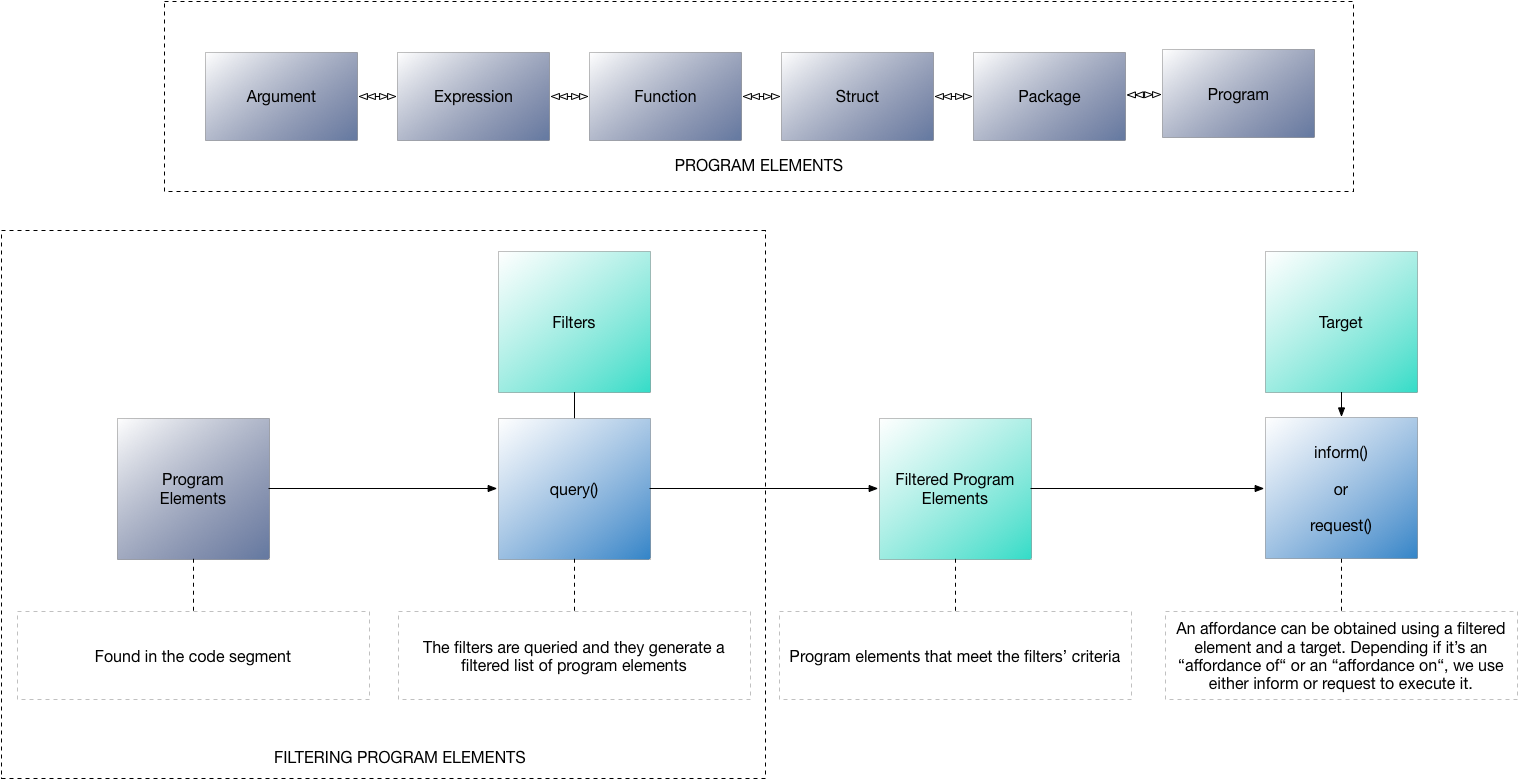
\includegraphics[width=1.0\textwidth]{img/affordances.png}
\label{figure:affordances-workflow}
\end{figure}

The current workflow of CX affordances is depicted in figure \ref{figure:affordances-workflow}. The topmost block in this figure shows all the program elements that can be used in this paradigm. Each of these types of elements can interact with any of the other types and with themselves. For example, we can ask for affordances between an argument and a function, as well as we can ask for affordances between an argument other arguments.

The block at the lower-left corner shows in figure \ref{figure:affordances-workflow} how the \textbf{query} function uses \emph{filter}s to generate a list of program elements. We can now use one of these elements in conjunction with a target to obtain an affordance. For example, an argument can replace another argument in a program, or we can use a structure and a function to create a new method.

The last part of figure \ref{figure:affordances-workflow} involves two functions: \textbf{inform} and \textbf{request}. Both of these functions are used to actually execute an affordance, but they handle "affordances of" and "affordances on" a target, respectively. An "affordance on" a target involves affordances that are going to mutate the target itself, and an "affordance of" a target involves affordances where the target is going to mutate its environment (other program elements).

\begin{lstlisting}[caption={A list of "affordances of" an argument},captionpos=b,label={listing:affordances-of}]
Replace targetExpr.Input.0 with targetExpr.Input.0
Replace targetExpr.Input.1 with targetExpr.Input.0
Replace targetExpr.Output.0 with targetExpr.Input.0
\end{lstlisting}

\begin{lstlisting}[caption={A list of "affordances on" an argument},captionpos=b,label={listing:affordances-on}]
Replace targetExpr.Input.1 with targetExpr.Input.0
Replace targetExpr.Input.1 with targetExpr.Input.1
Replace targetExpr.Input.1 with targetExpr.Output.0
\end{lstlisting}

To help illustrate the concepts of "affordances of" and "affordances on", we can have a look at listings \ref{listing:affordances-of} and \ref{listing:affordances-on}. Listing \ref{listing:affordances-of} shows what are the possible affordances of the first (0th) argument of an expression labeled as "targetExpr". As these are "affordances of", the target (\textit{targetExpr.Input.0}) is going to affect other program elements. In this case, we are listed with different arguments that can be replaced with our target. In the case of listing \ref{listing:affordances-on}, as it shows "affordances on" the target, the options show what arguments can replace the target. To list the possible "affordances of" or "affordances on", you can use the \textbf{aff.of} and \textbf{aff.on} functions, respectively (see listing \ref{listing:affordances-example1} for an example of their usage).

\begin{figure}
\caption{Combinations of "affordances of"}
\centering
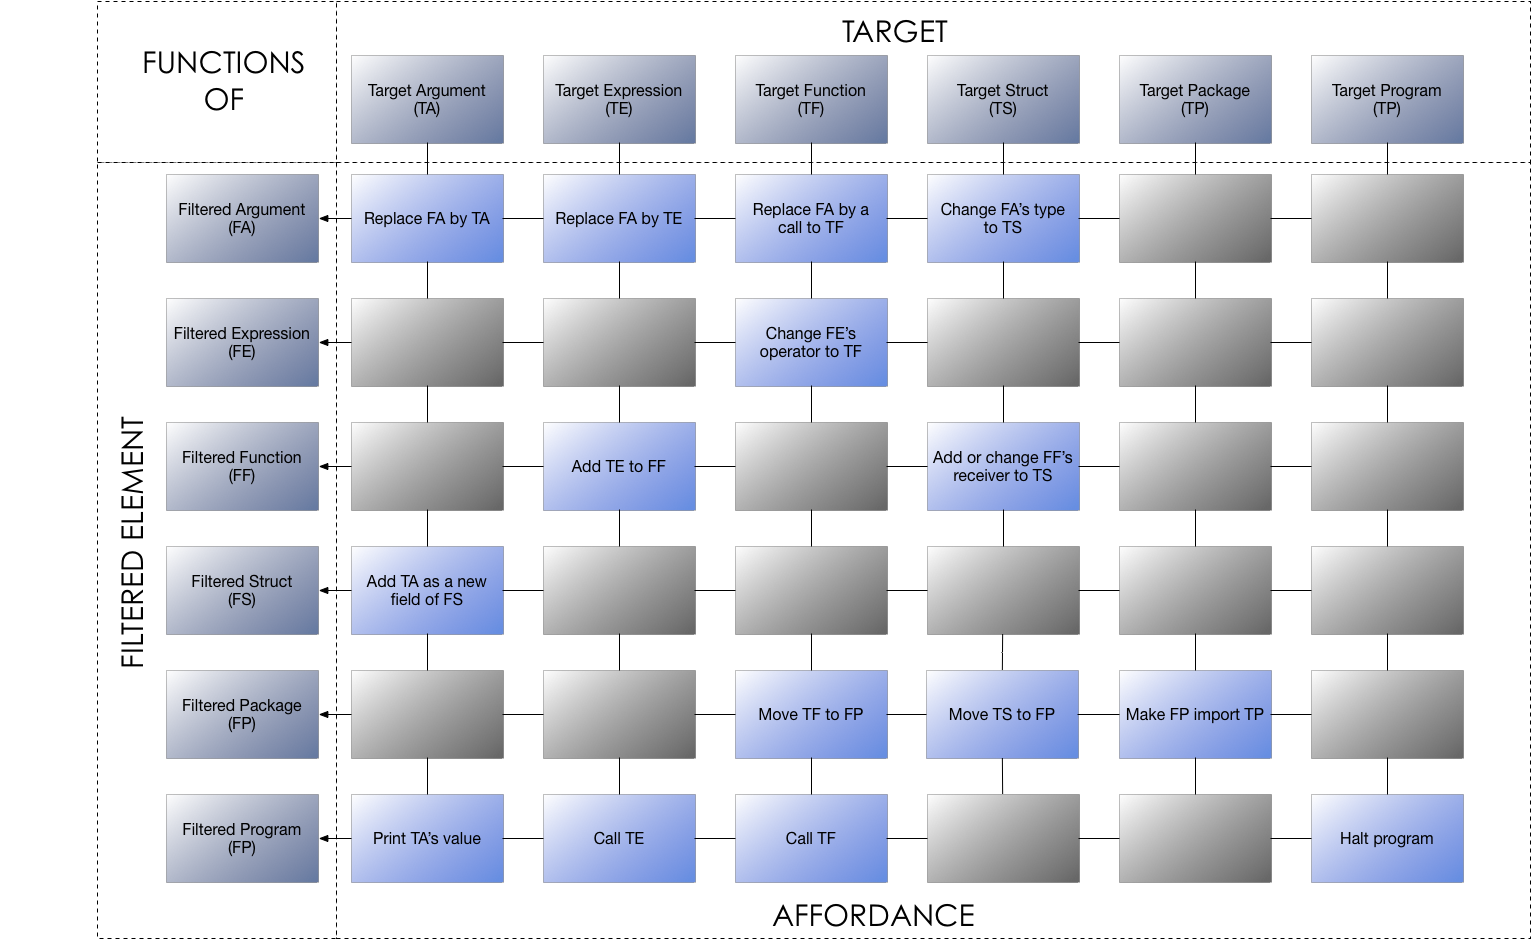
\includegraphics[width=1.0\textwidth]{img/functions-of.png}
\label{figure:combinations-of-affordances-of}
\end{figure}

\begin{figure}
\caption{Combinations of "affordances on"}
\centering
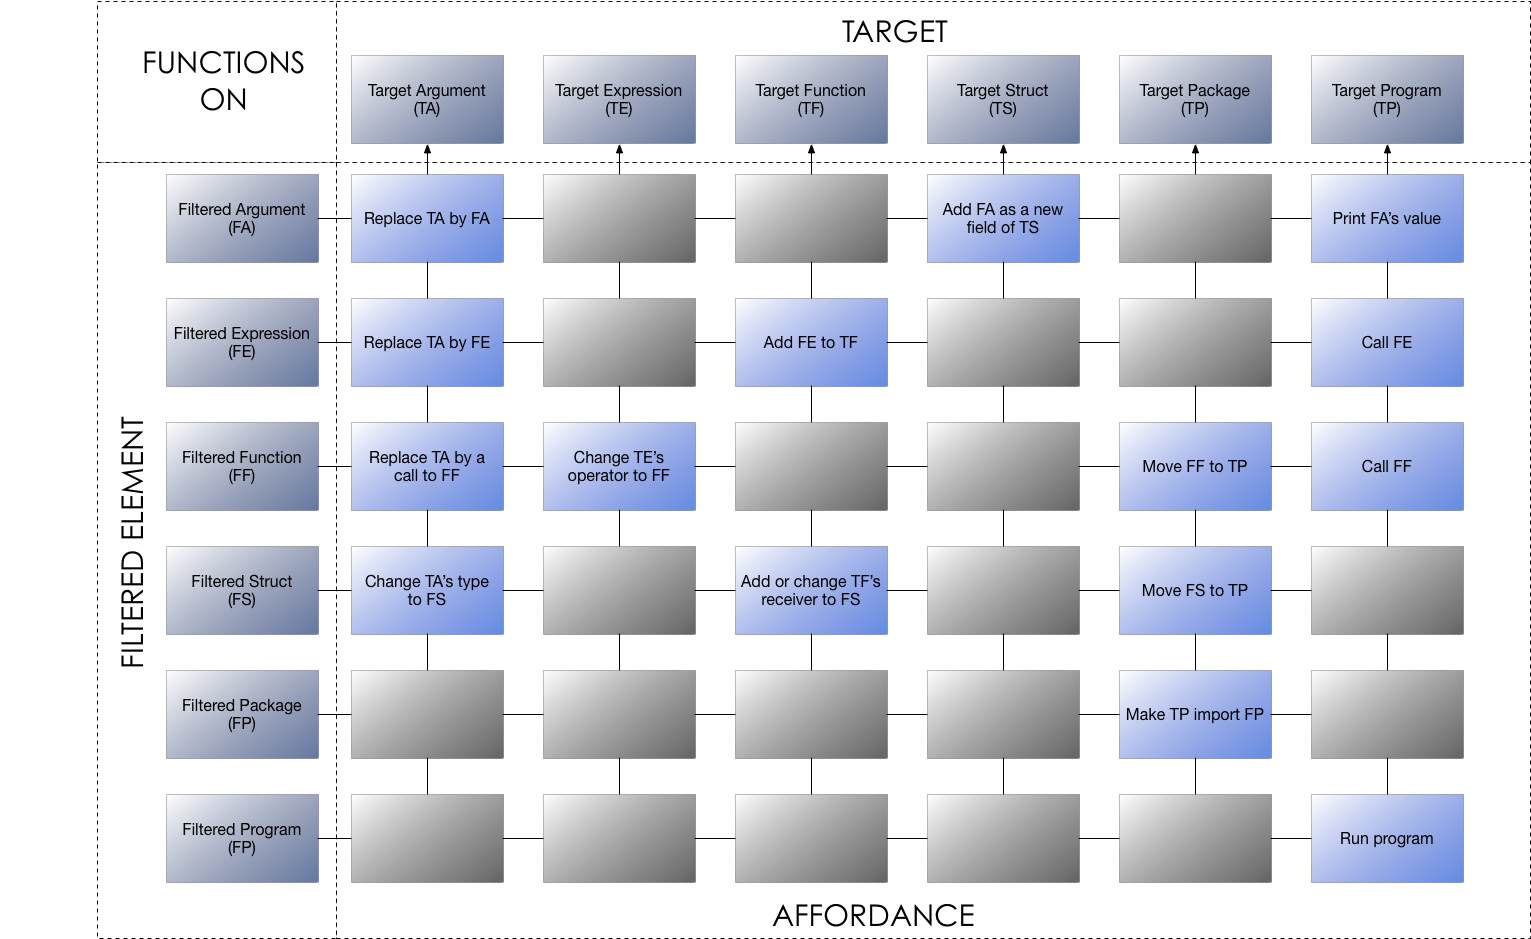
\includegraphics[width=1.0\textwidth]{img/functions-on.png}
\label{figure:combinations-of-affordances-on}
\end{figure}

Figures \ref{figure:combinations-of-affordances-of} and \ref{figure:combinations-of-affordances-on} show all the possible affordances that can occur between two program elements in CX. As can be seen, "affordances of" and "affordances on" can be considered as reciprocal operations.

\clearpage

\begin{lstlisting}[caption={Using affordances on an expression},captionpos=b,label={listing:affordances-example1}]
package main
import "aff"

func affIsI32 (arg aff.Argument) (res bool) {|\label{line:predarg-declaration}|
	if arg.Type == "i32" {
		res = true
	}
}

func main () {
	var foo i32
	
	tgt := #{|\label{line:aff-target1}|
		expr(targetExpr)
		inp(0)
	}

	fltrs := #{|\label{line:aff-filter1}|
		filter(affIsI32)
	}
	
	elts := aff.query(fltrs)|\label{line:aff-query1}|

	aff.of(elts, tgt) // show affordances of the target|\label{line:aff-of1}|
	// aff.on() // show affordances on the target|\label{line:aff-on1}|
	
	aff.request(elts, 1, tgt) // execute the second affordance on the target|\label{line:aff-request1}|
	// aff.inform(elts, 1, tgt) // execute the second affordance on the target|\label{line:aff-inform1}|

targetExpr:
	foo = i32.add(5, 6)|\label{line:aff-labeled-expr1}|

	i32.print(foo)
}
\end{lstlisting}

Listing \ref{listing:affordances-example1} shows an example of affordances involving arguments of an expression. In order to create a target, we will use the affordance operator: \emph{\#\{\}}. A target is created starting at line \ref{line:aff-target1} using this operator and a series of function calls. The function calls in this case are used to select the actual target, and they can be read as: from \lstinline{expr(targetExpr)}, target the 0th input (\lstinline{inp(0)}). If \lstinline{inp(0)} is not included, we would be targeting the expression as a whole, and not one of its arguments.

After having specified a target, we need to create filters that can be queried to generate program elements. In the case of this example, we are using only one filter: \lstinline{filter(affIsI32)}. The argument of \textbf{filter} needs to be a function that acts as a predicate, i.e. it needs to return a Boolean that tells if an element met certain criteria or not. The input argument to this predicate can be any of:

\begin{itemize}
    \item aff.Program
    \item aff.Package
    \item aff.Function
    \item aff.Argument
    \item aff.Expression
    \item aff.Structure
\end{itemize}

\textbf{predArg} is declared at line \ref{line:predarg-declaration}, and it is a predicate that is going to filter arguments, as it is declared to have an input parameter of type \textbf{aff.Argument}. This predicate has a very simple behavior: it checks if the argument is of type \emph{i32}; if it is, it returns \emph{true}, which means that the argument meets the filter's criteria; if it is not, it returns \emph{false}, which means that the argument does not meet the filter's criteria.

Now that we have a filter, we can query it, as shown in line \ref{line:aff-query1}. In this case, the result of the query is going to be stored in a variable called \textbf{elts}. If you want to print the contents of this variable or any other variable that is holding the output of the call of an affordance operator (\emph{\#\{\}}), you can use the function \textbf{aff.print}. For example, \lstinline{aff.print(elts)} will print the contents of this variable.

As shown in figure \ref{figure:affordances-workflow}, the two elements needed to execute an affordance are a target and a filtered program element, and we now have both of these. To check what are the possible affordances involving the target and each of the filtered elements, we can either call \textbf{aff.of} or \textbf{aff.on}, to print either the "affordances of" or "affordances on" the target, respectively. In the case of listing \ref{listing:affordances-example1}, we are printing to the terminal the "affordances of" the target, as can be seen in line \ref{line:aff-of1}. If you want to print the "affordances on" the target, you can un-comment line \ref{line:aff-on1}. The affordances that will be printed will resemble the ones shown in listings \ref{listing:affordances-of} and \ref{listing:affordances-on}.

Finally, in order to execute one of the possible affordances, we can either use \textbf{aff.inform} or \textbf{aff.request}, to execute either an "affordance of" or an "affordance on" the target, respectively. We can see how we can do both operations in lines \ref{line:aff-request1} and \ref{line:aff-inform1}, although the line calling \textbf{aff.inform} is commented out.

Without executing any affordances, the expression at line \ref{line:aff-labeled-expr1} would print an 11 to the terminal. But after executing the affordance, the expression will print 10. If we examine the second affordance shown in \ref{listing:affordances-of}, we can see that the operation to be performed is to "replace targetExpr.Input.1 with targetExpr.Input.0". In this case, \emph{targetExpr.Input.1} is the 6 being sent as the second argument to \textbf{targetExpr}, and \emph{targetExpr.Input.0} is the first argument, which is a 5. In other words, we are replacing the second input argument with the first input argument, which translates to \lstinline{foo = i32.add(5, 5)}.

In contrast, if we are interested in the "affordances on" the target (which is obtained by un-commenting the code in listing \ref{listing:affordances-example1}), we would be executing the second affordance shown in \ref{listing:affordances-on}, which is "replace targetExpr.Input.1 with targetExpr.Input.1", which should not change the program at all, as we are replacing the second input argument with itself. As a result, the program will print 11 to the terminal.

% Listing \ref{listing:affordances-example1} shows a basic program that uses affordances to filter among the possible values that the expression at \textbf{line \ref{line:affordance-expression}} can take. As this is a small program, the only possible values are those being held by \textbf{foo1}, \textbf{foo2} and \textbf{foo3}. In order to know what expression we want to target, we need to label it first. To do this, we can simply use to-do labels, as seen at \textbf{line \ref{line:affordance-label}}, where we label our target expression as "message." 
% The next step is to create a variable to hold the target expression. To do this, we use the affordance mini programming-language, which is called by writing \textbf{->\{\}}, and we write the desired statements inside of the braces. Creating a target is done at \textbf{line \ref{line:affordance-target}}. Targets are constructed by going down in levels of scope: the package is specified first, then the function, and lastly the expression. To specify the desired package, you use \textbf(pkg) followed by the name of the package enclosed by parentheses. For functions, you use \textbf{fn}, followed by the name of the function enclosed by parentheses. Lastly, to specify the expression, you use \textbf{exp} followed by the label given to the expression, again, enclosed by parentheses.

% Rules, as mentioned before, are used to filter the possible options. In this example, rules are defined at \textbf{line \ref{line:affordance-rules}}, and they contain only one clause: allow anything that is greater than \lstinline{1}. The asterisk in here represents the initial allowed objects to be sent to the targeted expression. As the expression is waiting for a 32-bit integer, the asterisk will be of type i32. Think about it like how the x in mathematics can mean any number but, in this case, it can mean any program element. If the targeted expression can receive a structure instance as its input, we could create predicates of the form \lstinline{*.field == something}, for example.

% Now that we have both the target and the rule set, we can query CX's affordance system using \textbf{aff.query}, as shown at \textbf{line \ref{line:affordance-query}}. The results returned by \textbf{aff.query} can be pretty-printed to the console by calling \textbf{aff.print}, as shown at \textbf{line \ref{line:affordance-print}}. This is useful if you want the user to be involved on what affordance to execute. For example, you could use affordances to create an entire program just by selecting the options that you want, and \textbf{aff.print} would be used to let the programmer know what affordance to execute. 

% When you have chosen an appropriate affordance, either manually or automatically, you can execute it by calling \textbf{aff.execute}, as shown at \textbf{line \ref{line:affordance-execute}}. \textbf{aff.execute} takes three arguments as inputs: a target, the set of affordances, and an index representing the desired option to execute. As you can see, you could execute the same affordance to several targets, and execute several affordances by specifying different indexes. In the case of the above example, we simply execute the first option, represented by index 0. After running the whole program, the number 2 should be printed to the console, as is the first element that is greater than 1.


\begin{lstlisting}[caption={Using affordances on an expression},captionpos=b,label={listing:affordances-example2}]
package main
import "aff"

func isMainBar (prgrm aff.Program) (res bool) {|\label{line:predprogram}|
  	if prgrm.Caller.FnName == "main.bar" && prgrm.Caller.FnSize == 0 {|\label{line:predprogram-cond}|
		res = true
	}
}

func foo () {
  	fltrs := #{
		filter(isMainBar)
  	}
  	affs := aff.query(fltrs)
  	if len(affs) < 1 {
  		return
  	}
	
  	str.print(`I will only print if "main.bar" calls me`)
}

func bar () {
 	foo()
}

func main () {
  	foo()
  	bar()
}
\end{lstlisting}

Affordances can also be useful without any calls to \textbf{aff.inform} or \textbf{aff.request}. Listing \ref{listing:affordances-example2} shows an example of this, where we use the program's meta-data to determine if we should execute the body of a function or not. The predicate declared at line \ref{line:predprogram} has an input parameter of type \textbf{aff.Program}, which holds meta-data about the running program. In this case, as can be seen in line \ref{line:predprogram-cond}, we are going to "accept" the program only if the caller of the function (the function calling this filter) is named "main.bar" (the function \textit{bar} from the package \textit{main}) and if the size of the caller is 0 (which means that it has no variable declarations at all).

As can be seen in the body of \textbf{foo}, we create a filter that will call \textbf{prgrmPredicate}, we query it and store the result in \textbf{affs}. Then we simply determine if the result of querying the filter has returned any program elements by checking the length of \textbf{affs}. If the length is 0, this means that the caller of \textbf{foo} is not \textbf{bar} and that the caller's size is not equal to 0. As a consequence, we do not run the rest of the expressions contained in \textbf{foo}'s body. If you run code in listing \ref{listing:affordances-example2}, you should see the message 'I will only print if "main.bar" calls me' printed to the terminal only once, although we actually called \textbf{foo} twice.

% Listing \ref{listing:affordances-example2} shows a much more complex example. The program is an extremely naive representation of a robot moving on a map. The map is built using two arrays, where each of the indexes represents a room, and the indexes "surrounding" them are used as the contiguous rooms. One of the arrays has walls, and the other one wormholes. If the robot encounters a wall on the map, it cannot move to that direction, but if a wormhole is on the wall, it can move to the other side. In the arrays, a true value means that a wall or a wormhole is present there, and a false means there is not. In the example, there is no wormhole, so you can play with the values to see the different results.

%----------------------------------------------------------------------------------------
%	CHAPTER 12
%----------------------------------------------------------------------------------------

% % \chapterimage{blank-header.png}
% \chapter{Object Explorer}
% \label{chapter:object-explorer}

% \begin{remark}
% Section Outline
%     \begin{itemize}
%     	\item Now that I explained affordances and the garbage collector, we can move on to a very interesting tool that CX will provide: the object explorer
%         \item The object explorer is an API that can be queried to obtain a list of objects present and alive in the heap
%         \item You can use this API to make any application you want (that uses the API), but...
%         \item CX also provides a web application that connects to this API, where you can see all the objects graphically
%         \item In this web app, you'll be able to use affordances on the objects
%         \item The object explorer will usually be used in combination with stepping and the REPL
%         \item Stepping will help us to stop a running application, query the object explorer, perform any affordances on the objects, and then continue with the program execution
%     \end{itemize}
% \end{remark}

% CX's object explorer is an API that can be queried to obtain a list of the objects present in the heap and the stack. It is very useful for debugging a program, as you can pause its execution, enter the REPL, and start examining the current state of the program.

% The object explorer is still under heavy development

%----------------------------------------------------------------------------------------
%	CHAPTER 13
%----------------------------------------------------------------------------------------

% \chapterimage{blank-header.png}
\chapter{Serialization}
\label{chapter:serialization}
\index{serialization}

% \begin{remark}
% Section Outline
%     \begin{itemize}
%     	\item CX comes with object serialization included
%         \item In this case, any object in the program structure is capable of being serialized
%         \item For example, we can serialize functions, packages or a whole program
%         \item Although perhaps the most frequent operation would be to serialize struct instances to be saved to files
%         \item However, something interesting is that we could serialize a full program, send it to another server, deseralize it there, and continue its execution there
%         \item Another interesting use is that we could have a distributed application that evolves functions (see chapter \ref{chapter:genetic-programming}), and sends these evolved functions to a central server
%         \item At the moment, one can only serialize full programs or struct instances in CX
%         \item Show serialization examples (program and struct instances)
%         \item \textbf{NOTE} I need to clean up the struct serialization example
%     \end{itemize}
% \end{remark}

In CX, every program object and piece of data can be serialized at any moment, preserving any state in which the program is. You can choose to serialize all the program or only certain parts of it, such as structure instances or functions. These serialization features are very useful, as you can save a program to a file or a database - or a blockchain on Fiber\footnote{Fiber is the system used by the Skycoin blockchain to allow other blockchains to be used on top of it. This is similar to the ERC-20 tokens' blockchains that run on ethereum}.

The serialization process not only involves the program structure, e.g. function declarations and structure instances. Other parts of a CX program are also serialized, such as the call stack and the different memory segments in CX. This means that a program can be totally or partially serialized, and it can resume its execution later on. A program could be paused, serialized and sent over a network to different computers to be executed in there. A common example of CX's serialization combined with other of CX's features is as follows.

Imagine you want to evolve programs to predict a financial market's price movement. You can start evolving functions inside of a CX program using its integrated genetic programming system (see chapter \ref{chapter:genetic-programming}). At certain points in time you can save these serializations to a database, for example, programs which achieved a very good performance. You can then send some of these serializations to other workstations or servers where they will initialize a separate evolutionary process. This is something similar to taking some monkey from Earth to different planets in the Universe: wait a few millions of years, and then check how they evolved in each of these planets{only if you believe in the theory of evolution, though; otherwise, they will still be monkeys}.

Evolutionary algorithms can often be manually manipulated (imagine aliens interfering with the DNA of a planet's species). A person can log in to one of the workstations or servers in this evolutionary network, and check some of the individuals being evolved in CX. This person will just have to pause the program using the CX REPL, and check the program's structure using the \textbf{:dp} meta-command (see chapter \ref{chapter:mastering-the-repl}). But maybe this person does not know what can be added or removed from the function being evolved. This is not a problem, because the function is evolving according to a rule set established in CX's affordance system (see chapter \ref{chapter:affordances}, and you would only need to call the affordance system in the CX REPL and start selecting options from a menu. After being happy with the changes, the program can be resumed again by issuing the meta-command \textbf{:step 0}, so the program continues its execution (see chapter \ref{chapter:mastering-the-repl}).

% Finally, imagine that some days have already passed and you want to update the data being fed to your system. You can call CX's object explorer to update the arrays of data (see chapter \ref{chapter:object-explorer}). Then you can serialize your program's data, and propagate the changes to the other servers.

\section{Serialization}
\label{section:serialization}

Now let us see how you can serialize the different program elements and data in CX.

\begin{lstlisting}[caption={Serialization of a program},captionpos=b,label={listing:serialization-program}]
package main

func main () {
    var target aff
    var result []byte
    
    target = #{}
    result = serialize(target)
}
\end{lstlisting}

Listing \ref{listing:serialization-program} shows how to serialize a full program using the function \textbf{serialize}, which is the one that we are going to be using in all the subsequent examples. We can tell the function \textbf{serialize} what to serialize by using the affordance operator (\textbf{->}) (see chapter \ref{chapter:affordances}). In the case of serialization, we are only going to be using the affordance operator to specify a target to be serialized. In the case of listing \ref{listing:serialization-program}, we are leaving the target empty. This is a special case that instructs CX to serialize everything or, in other words, the full program.

\begin{lstlisting}[caption={Serialization of a package},captionpos=b,label={listing:serialization-package}]
package main

func main () {
    var target aff
    var result []byte
    
    target = #{pkg(main)}
    result = serialize(target)
}
\end{lstlisting}

If your program only has one package, as in listing \ref{listing:serialization-package}, you could end up with a similar serialization as in listing \ref{listing:serialization-program}, but with some differences. \lstinline|#{}| instructs CX to serialize \emph{everything}, including CX's memory segments (see chapter \ref{chapter:garbage-collector}), whereas \lstinline|#{pkg(main)}| is only going to cause a serialization of the program segment (the program structure).

\begin{lstlisting}[caption={Serialization of the memory segments},captionpos=b,label={listing:serialization-memory-segments}]
package main

func main () {
    var target aff
    var result []byte
    
    target = #{mem(heap)}
    result = serialize(target)
    
    target = #{mem(stack)}
    result = serialize(target)
    
    target = #{mem(data)}
    result = serialize(target)
}
\end{lstlisting}

To serialize the other memory segments, you can use the affordance target \textbf{mem()}, and give either \emph{heap}, \emph{stack} or \emph{data} as its argument, as seen in listing \ref{listing:serialization-memory-segments}.

It is worth noting that if you serialize your stack, you are actually serializing \emph{all} the stacks. CX, at the time of writing, is still not a multi-threaded programming language. Nevertheless, it should soon become one, and the data contained in all of the stacks will be serialized. Additionally, CX manages its call stack and stack separately, but both of these segments are serialized together when calling \textbf{serialize} with \textbf{mem(stack)}.

In later versions of CX, we might introduce native functions to process information from these serialization results, but for now, you can only deserialize this information into another instance of a CX program (see the next section) or process the byte slice byte by byte to do whatever you require to do.

\begin{lstlisting}[caption={Serialization of declarations},captionpos=b,label={listing:serialization-declarations}]
package main

var foo i32

func bar () {
    str.print("Hi.")
}

type foobar struct {
    foo i32
}

func main () {
    var target aff
    var result []byte

    target = #{
        pkg(main)
        var(foo)
    }
    result = serialize(target)
    
    target = #{
        pkg(main)
        fn(bar)
    }
    result = serialize(target)
    
    target = #{pkg(main) strct(foobar)}
    result = serialize(target)
}
\end{lstlisting}

Listing \ref{listing:serialization-declarations} shows how to serialize declarations in packages. Note that the structure and function serializations are serializing the code representation of these declarations, and not instances of these. In other words, if we were talking about structures, we would be serializing structure declaration itself and not an instance of the structure. In the case of the function declaration, CX does not have functions as first-class objects yet, so there should not be any confusion, but it's good to notice that we are referring to the function declaration itself, and not an instance of this function.

\begin{lstlisting}[caption={Serialization of expressions},captionpos=b,label={listing:serialization-expressions}]
package main

type Point struct {
    x i32
    y i32
}

func main () {
    var target aff
    var result []byte
    
    var foo i32
    var bar Point
    
foobar:|\label{line:serialization-label-expression}|
    i32.print(foo)

    target = #{
        pkg(main)
        fn(main)
        var(foo)
    }
    result = serialize(target)
    
    target = #{
        pkg(main)
        fn(bar)
        var(bar)
    }
    result = serialize(target)
    
    target = #{pkg(main) fn(bar) expr(foobar)}
    result = serialize(target)
}
\end{lstlisting}

Lastly, you can also serialize function statements, expressions and variable declarations. As you can see in listing \ref{listing:serialization-expressions}, function variables are targeted by specifying the package, the function and the name of the variable using \textbf{pkg}, \textbf{fn} and \textbf{var} in the affordance operator, respectively. The case of targeting an expression is a bit more complex, as you need to label it first (\textbf{line \ref{line:serialization-label-expression}}), and then use that label to target the expression in the affordance operator.

\section{Deserialization}
\label{section:deserialization}
\index{deserialization}

After serializing program elements or data using the procedures described in the last section, you may now want to deserialize the resulting slices of bytes.

\begin{lstlisting}[caption={Deserialization of a program},captionpos=b,label={listing:deserialization-program}]
package main

func main () {
    var target aff
    var result []byte
    
    target = #{}
    result = serialize(target)
    deserialize(result)
}
\end{lstlisting}

We're not going to be deserializing all of the examples from the last section, as it would be pointless. You are always going to have a slice of bytes, and they are always going to be deserialized by the \textbf{deserialize} function. Listing \ref{listing:deserialization-program} shows \textbf{deserialize} in action, which is deserializing a slice of bytes representing the whole program.

What \textbf{deserialize} does is something similar to a \emph{patch}. If a declaration in the slice of bytes already exists in the current program, it will simply redefine it; if it does not exist, it will create it. In the case of function declarations, statements and expressions, they can be applied using the affordance system, although this functionality has not been implemented yet.

%----------------------------------------------------------------------------------------
%	CHAPTER 15
%----------------------------------------------------------------------------------------

% \chapterimage{blank-header.png}
\chapter{CX Base Language}
\label{chapter:creating-your-own-cx}
\index{base language}

% \begin{remark}
% Section Outline
%     \begin{itemize}
%     \item We need to recall from chapter \ref{chapter:getting-started-with-cx} that CX is first a programming language specification and that the language that we have been using throughout the book is an implementation of that specification: CXGO
%     \item Skycoin provides a set of functions (describe it better) that you can use to construct a program structure, and a runtime that you can use to run it
%     \item CXGO Uses Bison to parse its programs, but in this chapter we will see how we can create a visual programming language that generates a CX program structure that can be run by the runtime
%     \item Describe the process
%     \end{itemize}
% \end{remark}

In chapter \ref{chapter:introduction} we mentioned that CX is actually a programming language specification, which means that you could create your own CX. The CX that we have been using throughout the book to run all the examples is called CXGO (something similar to how the most popular Python implementation is actually called CPython).

At the moment, the specification file has not been finished and it needs to be heavily updated, which means that creating your own CX from scratch is not possible, as you would not know what conditions need to be met by your language. But fear not, because you can use the official Skycoin implementation to create it!

CX does not specify any syntax or grammar to be followed, which means that you could even create a CX in Minecraft using redstone. In order for a language to be called CX, it only needs to implement the necessary native functions and follow the same program structure as any other CX. For example, your CX cannot implement classes, as they do not exist in CX. Also, you would be required to implement an affordance system, as this feature is required in all CX programming language implementations.

How programs are executed in CX is also unspecified, which means that you could build your own runtime, compiler, linker, etc. However, you are required to compile to the same program structure. The objective with this approach is to have any program created in any CX to run using any runtime system. This is similar to the approach that some languages like Clojure or F\# take, where they run using the JVM or the CLR, respectively.

Skycoin's CX implementation is divided in two parts: a library that can be used to construct programs to be run in CX, called the \emph{CX base}, and the programming language parser/interpreter/compiler, which was created using the CX base language and a parser built in \emph{goyacc} and Go. If you do not mind programming in Go, you can import the CX base language to create a CX implementation.

\begin{lstlisting}[caption={Writing a program using CX base language},captionpos=b,label={listing:cx-base-program}]
package main

import (
	. "github.com/skycoin/cx/cx"|\label{line:cx-base-import}|
)

func main () {
	prgrm   := MakeProgram()|\label{line:base-program}|
	mainPkg := MakePackage("main")|\label{line:base-package}|
	mainFn  := MakeFunction("main")|\label{line:base-function}|

	prgrm.AddPackage(mainPkg)|\label{line:base-add-package}|
	mainPkg.AddFunction(mainFn)|\label{line:base-add-function}|

	prgrm.RunCompiled()|\label{line:base-run}|
}
\end{lstlisting}

Listing \ref{listing:cx-base-program} shows how you can use the CX base language to create a very basic program that can be run using Skycoin's CX runtime. First we need to import the CX base language package, as shown at \textbf{line \ref{line:cx-base-import}}. This package will give us access to \emph{makers}, \emph{adders}, \emph{removers} and other utility functions that will help us construct a compliant CX program. \textbf{line \ref{line:base-program}} creates the minimal CX program you could create: a null program. A null program is one that does not have any package, functions or anything in it. If you try to run this program, CX will complain because it does not have a \emph{main} package nor a \emph{main} function, but this does not mean it is not a valid CX program; if you were developing a library, neither of these two components would be required.

As we are interested in creating a running program, not just a library, we create a \emph{main} package and function, at \textbf{lines \ref{line:base-package}} and \textbf{\ref{line:base-function}}, respectively. As you can see, the naming convention for the functions that are going to be creating the program elements is \emph{MakeXXX}, and these functions will usually require the essential properties to be sent as input parameters, such as the name of a package.

We already have the elements created, but they have not been added to the main program structure yet. We can do this by calling an adder method on the elements that are going to hold these new elements. In this case, we are interested on adding a function to a package, and adding that package to the main program structure. To do this, we're calling the program's method \textbf{AddPackage}, and sending the created package as an argument, and we do the same with the \emph{main} function by calling the package's method \textbf{AddFunction}, and sending it as an argument. These operations are seen at \textbf{lines \ref{line:base-add-package}} and \textbf{\ref{line:base-add-function}}.

Finally, even though the program does nothing, we run the program by calling the program's method \textbf{RunCompiled} at \textbf{line \ref{line:base-run}}. Save that code to a file, run it by executing \lstinline{go run example.go}, and you should see... nothing. Let us now create a more interesting program: let us calculate 10 + 10!

\begin{lstlisting}[caption={Summing 10 + 10 using CX base language},captionpos=b,label={listing:cx-base-sum}]
package main

import (
	. "github.com/skycoin/cx/cx"
)

func main () {
	prgrm := MakeProgram()|\label{line:your-own-start}|
	mainPkg := MakePackage("main")
	mainFn := MakeFunction("main")
	initFn := MakeFunction(SYS_INIT_FUNC)

	prgrm.AddPackage(mainPkg)
	mainPkg.AddFunction(mainFn)
	mainPkg.AddFunction(initFn)|\label{line:your-own-end}|

	sum := MakeExpression(Natives[OP_I32_ADD], "", 0)|\label{line:your-own-sum-expression}|

	num := MakeArgument("", "", 0)|\label{line:your-own-num}|
	num.AddType("i32")
    num.Offset = 0|\label{line:your-own-offset}|

	WriteToStack(&prgrm.Stacks[0], 0, []byte{10, 0, 0, 0})

	sum.AddInput(num)|\label{line:your-own-input1}|
	sum.AddInput(num)|\label{line:your-own-input2}|

	result := MakeArgument("result", "", 0)|\label{line:your-own-result}|
	result.AddType("i32")
	sum.AddOutput(result)|\label{line:your-own-add-output}|
	
	prnt := MakeExpression(Natives[OP_I32_PRINT], "", 0)|\label{line:your-own-i32-print}|
	prnt.AddInput(result)|\label{line:your-own-i32-print-add-input}|

	mainFn.AddExpression(sum)|\label{line:your-own-add-sum}|
	mainFn.AddExpression(prnt)|\label{line:your-own-add-prnt}|

	prgrm.RunCompiled(0)
}
\end{lstlisting}

Listing \ref{listing:cx-base-sum} shows how you can double a number, and then print the result using the CX base language. This is an example on how you can use a program to write other programs that can be executed immediately.

Similarly to the last example, we need to create a program, a \emph{main} package, and a \emph{main} function. In addition to that, we need to create an \emph{*init} function, which, as explained in chapter \ref{chapter:cx-programs-representation}, initializes some parts of a CX program such as global variables. These components are created and added to the program at \textbf{lines \ref{line:your-own-start}-\ref{line:your-own-end}}. Then we continue with the expression that will perform the sum at \textbf{line \ref{line:your-own-sum-expression}}.

As mentioned before, we will be doubling a generic number (which happens to be 10), not just doubling 10. Let us see how we create the inputs. First, we need to create the argument at \textbf{line \ref{line:your-own-num}}. The first input argument to \textbf{MakeArgument} is the name of the argument, which only makes sense if we're creating a variable or symbol. In this case we just want to hold a reference to the number 10, so we do not really need to name the argument. Additionally, we already have the internal name of this argument, as we are assigning it to the Go variable \textbf{num}.

\textbf{num} will be pointing to the \emph{offset} 0, as seen at \textbf{line \ref{line:your-own-num}}. This means that whatever is stored at the beginning of a stack frame, that will be the value of our \textbf{num} argument, and as it is of type \emph{i32}, it will have a size of 4, which means that CX will read the first 4 bytes of the stack frame. Before continuing with the next parts, the second and third arguments of \textbf{MakeArgument} are the file name where the argument is declared and line number respectively, which we do not need for this example.

Next we will write our information to the stack. To do this, we will use the function \textbf{WriteToStack}, which first takes a stack as its argument, then the offset at which it should start writing bytes, and lastly the sequence of bytes to write. As has been mentioned in other chapters, CX is currently single-threaded, but future versions will become multi-threaded. As a consequence of this, you need to send \textbf{WriteToStack} a reference to the stack to which you want to write to. For this example, we are using the first stack, we will start writing our bytes at the index 0 of the stack, and we will write \lstinline{10, 0, 0, 0}, which corresponds to the 32-bit integer 10 (least significant byte first).

After creating the argument and writing the bytes our argument will be pointing to, we can now add this argument to our expression. This is done at \textbf{lines \ref{line:your-own-input1}} and \textbf{\ref{line:your-own-input2}}. As you can see, we are adding the same argument twice to the expression (we want to be efficient with our memory, after all).

If we run the program until this point, CX will complain about evaluating the expression and not using the result, similarly to what Go would throw. Let us now assign the result to a variable to avoid this error. To do this, we create another argument, as seen at \textbf{line \ref{line:your-own-result}}, and then we add this argument as the \textbf{sum} expression's output, as seen at \textbf{line \ref{line:your-own-add-output}}.

Now if we run the program until this point, we will have CX doubling 10, and overwriting this number with 20. The reason behind this is that the output variable \textbf{result} has a default offset of 0 too, so it is pointing to the same memory address as \textbf{num}.

The next expression does a call to \textbf{i32.print}, and is defined at \textbf{line \ref{line:your-own-i32-print}}. After defining the expression, we can add an input argument to it which, in this case, is the \textbf{result} argument, as seen at \textbf{line \ref{line:your-own-i32-print-add-input}}.

So far, it has been an exhaustive journey, but the only thing left now is to add the expressions to our \emph{main} function, as it is done at \textbf{lines \ref{line:your-own-add-sum}} and \textbf{\ref{line:your-own-add-prnt}}, and call our program's \textbf{RunCompiled} method. Finally, if we run our file with \lstinline{go run example.go}, we will see a 20 being printed to the terminal. Feel proud about your achievement!

As a final comment, if you want to create your own CX, you will need to generate all these commands automatically. For example, you can use a parser such as \emph{goyacc} (the one used by CXGO) to generate the program's structure. 

%----------------------------------------------------------------------------------------
%	CHAPTER 8
%----------------------------------------------------------------------------------------

% \chapterimage{blank-header.png}
\chapter{Standard Library}

----FIXME: Write an introduction

\section{Os}
\label{section:library-os}
\index{library os}
\index{os library}

\section{Time}
\label{section:library-time}
\index{library time}
\index{time library}

\section{Http}
\label{section:library-http}
\index{library http}
\index{http library}

\section{Affordances}
\label{section:library-aff}
\index{library aff}
\index{aff library}

\section{Serialization}
\label{section:library-serial}
\index{library serial}
\index{serial library}

\section{OpenGL GLFW and GLText}
\label{section:library-opengl}
\index{OpenGL}
\index{GLFW}
\index{GLText}

% \begin{remark}
% Section Outline
%     \begin{itemize}
%     \item \emph{CONSIDER} It might be a good idea to move this section to the first chapters. This consideration gains more weight if we manage to include video games in all of the chapters
%     	\item We all love video games in the CX team. That's why we decided to implement bindings to OpenGL and GLFW to test the language capabilities
%         \item In order to start using functions from these libraries, you only need to import "gl" and "glfw"
%         \item Let's review this first example, where we only open a window where we will be able to draw to later on
%         \item Review the listing's code, almost line by line
%         \item Review the other listings in the same way
%     \end{itemize}
% \end{remark}

In the Skycoin team we believe that a bright future exists for blockchain technologies in video game development. For this reason, one of the first libraries that was developed for CX was the OpenGL library. This chapter presents some video game examples that should help you get started with video game development in CX. In order to use the OpenGL and GLFW libraries in your CX programs, just \lstinline{import "gl"} and \lstinline{import "glfw"} after the package declaration.

The current OpenGL library does not implement all of the OpenGL functions and constants, but in future versions, this will be corrected. The OpenGL version that the CX library targets is 2.1.

CX also provides a GLFW library that helps the programmer set up things like windows and input devices. The GLFW version targeted by the CX library is 3.2.

The examples in this chapter are not explained thoroughly, as the purpose of this book is to explain the features of the CX programming language, not to explain how OpenGL and GLFW work.

\begin{lstlisting}[caption={Creating a window using OpenGL},captionpos=b,label={listing:window-opengl}]
package main

import "gl"
import "glfw"

var width i32 = 800|\label{line:window-example-width}|
var height i32 = 600|\label{line:window-example-height}|

func main () {
	glfw.Init()
	glfw.WindowHint(glfw.Resizable, glfw.False)
	glfw.WindowHint(glfw.ContextVersionMajor, 2)
	glfw.WindowHint(glfw.ContextVersionMinor, 1)

	glfw.CreateWindow("window", width, height, "Window Example")|\label{line:window-example-create}|
	glfw.MakeContextCurrent("window")
	
	gl.Init()
	var program i32
	program = gl.CreateProgram()
	gl.LinkProgram(program)
	
	for bool.not(glfw.ShouldClose("window")) {|\label{line:window-example-loop}|
		gl.Clear(i32.bitor(gl.COLOR_BUFFER_BIT, gl.DEPTH_BUFFER_BIT))

		gl.UseProgram(program)

		glfw.PollEvents()
		glfw.SwapBuffers("window")
	}
}
\end{lstlisting}

The first step to creating a video game is to create the window where everything is going to be displayed. Listing \ref{listing:window-opengl} shows a bare-bones example that only displays an empty window. You could think that this is a lot of instructions to only accomplish a simple task such as creating a window, but it is the OpenGL way. This example can be used as a template to start a new OpenGL project in CX.

The window has a resolution of 800x600, as defined by the global variables \textbf{width} and \textbf{height}, at \textbf{lines \ref{line:window-example-width} and \ref{line:window-example-height}}, respectively. The function that actually creates the window to be displayed is created at \textbf{line \ref{line:window-example-create}}, and it is constantly being re-drawn in the loop that begins at \textbf{line \ref{line:window-example-loop}}.

\begin{lstlisting}[caption={Drawing a triangle to a window},captionpos=b,label={listing:triangle}]
package main

import "gl"
import "glfw"

var width i32 = 800
var height i32 = 600

func main () () {
	glfw.Init()

	glfw.CreateWindow("window", width, height, "Triangle")
	glfw.MakeContextCurrent("window")
	
	gl.Init()
	
	var program i32
	program = gl.CreateProgram()
	
	gl.LinkProgram(program)

	for bool.not(glfw.ShouldClose("window")) {
		gl.Clear(gl.COLOR_BUFFER_BIT)

		gl.UseProgram(program)
		
		gl.MatrixMode(gl.PROJECTION)|\label{line:start-triangle}|
		gl.LoadIdentity()
		gl.MatrixMode(gl.MODELVIEW)

		gl.Begin(gl.TRIANGLES)
		gl.Color3f(1.0, 0.0, 0.0)
		gl.Vertex3f(-0.6, -0.4, 0.0)
		gl.Color3f(0.0, 1.0, 0.0)
		gl.Vertex3f(0.6, -0.4, 0.0)
		gl.Color3f(0.0, 0.0, 1.0);
		gl.Vertex3f(0.0, 0.6, 0.0);
		gl.End();|\label{line:end-triangle}|
		
		glfw.PollEvents()
		glfw.SwapBuffers("window")
	}
}
\end{lstlisting}

\begin{figure}
\caption{Triangle in OpengGL window}
\centering
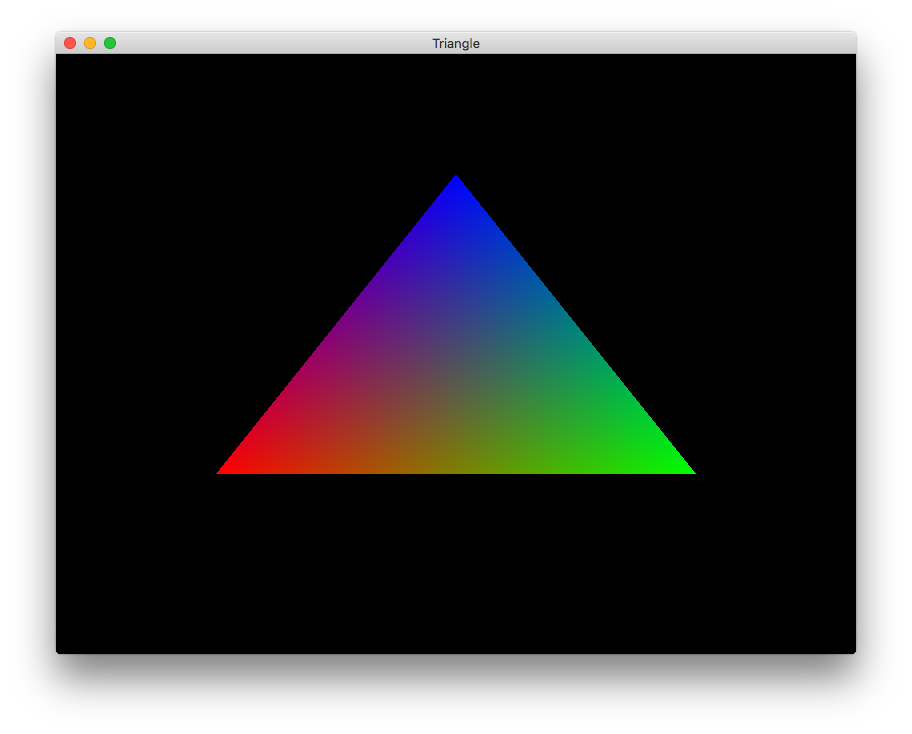
\includegraphics[width=0.5\textwidth]{img/opengl-triangle.png}
\label{figure:triangle}
\end{figure}

Now that we can create a window and display it, let us draw something on it. Listing \ref{listing:triangle} adds some lines of code to the code in listing \ref{listing:window-opengl} (\textbf{lines \ref{line:start-triangle} - \ref{line:end-triangle}}). Functions \textbf{gl.Color3f} and \textbf{gl.Vertex3f} are used to assign a color and coordinates to a vertex for a triangle, enclosed by calls to \textbf{gl.Begin} and \textbf{gl.End}. After running the code in this listing, you should see a window with a triangle like in the one displayed in figure \ref{figure:triangle}.

\begin{lstlisting}[caption={Bouncing ball example},captionpos=b,label={listing:bouncing-ball}]
package main

import "gl"
import "glfw"

var width i32 = 800
var height i32 = 600

type Ball struct {|\label{line:ball-struct}|
	x f32
	y f32
	vx f32
	vy f32
	gravity f32
	radius f32
}

func drawBall (ball Ball) () {
	var full_angle f32
	full_angle = f32.mul(2.0, 3.141592654)
	var x f32
	var y f32

	gl.Begin(gl.POLYGON)
	gl.Color3f(1.0, 1.0, 1.0)

	var i f32
	for i = 0.0; f32.lt(i, 20.0); i = f32.add(i, 1.0) {
		x = f32.add(ball.x,
		            f32.mul(ball.radius,
		                    f32.cos(f32.div(f32.mul(i, full_angle), 20.0))))
		y = f32.add(ball.y,
		            f32.mul(ball.radius,
		                    f32.sin(f32.div(f32.mul(i, full_angle), 20.0))))

		gl.Vertex2f(x, y)
	}

	gl.End()
}

func main () () {
	glfw.Init()

	glfw.CreateWindow("window", width, height, "Bouncing Ball")
	glfw.MakeContextCurrent("window")
	
	gl.Init()
	var program i32
	program = gl.CreateProgram()
	gl.LinkProgram(program)

	var ball Ball
	ball = Ball{
		radius: 0.05,
		x: 0.0,
		y: 0.0,
		vx: 0.01,
		vy: 0.01,
		gravity: 0.01}

	for bool.not(glfw.ShouldClose("window")) {|\label{line:bouncing-ball-start-loop}|
		gl.Clear(gl.COLOR_BUFFER_BIT)

		gl.UseProgram(program)
		
		gl.MatrixMode(gl.PROJECTION)
		gl.LoadIdentity()
		gl.MatrixMode(gl.MODELVIEW)

		if f32.lteq(f32.add(ball.y, ball.radius), -1.0) {
			ball.vy = f32.abs(ball.vy)
		} else {
			ball.vy = f32.sub(ball.vy, ball.gravity)
		}

		ball.x = f32.add(ball.x, ball.vx)
		ball.y = f32.add(ball.y, ball.vy)

		drawBall(ball)
		
		glfw.PollEvents()
		glfw.SwapBuffers("window")
	}|\label{line:bouncing-ball-end-loop}|
}
\end{lstlisting}

\begin{figure}
\caption{Bouncing ball in OpengGL window}
\centering
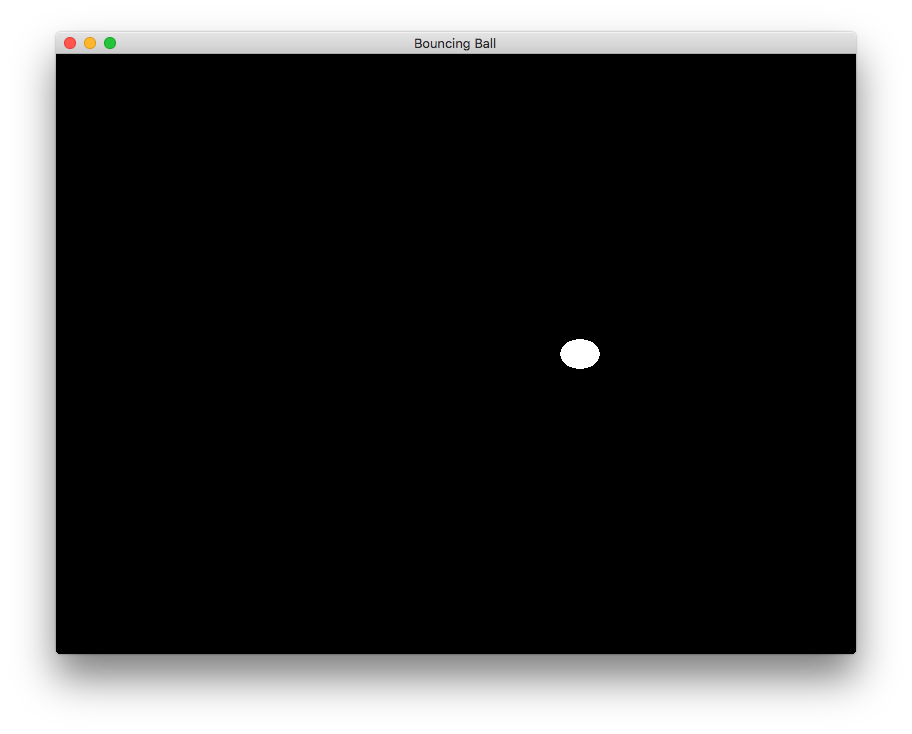
\includegraphics[width=0.5\textwidth]{img/bouncing-ball.png}
\label{figure:bouncing-ball}
\end{figure}

As the final example of this chapter, listing \ref{listing:bouncing-ball} presents a little more complex situation. We use a structure that will represent a ball to be drawn on screen, declared at \textbf{line \ref{line:ball-struct}}. In the for loop that updates the screen (\textbf{lines \ref{line:bouncing-ball-start-loop}-\ref{line:bouncing-ball-end-loop}}) we update the coordinates (x and y) of the ball, and draw the ball's new position to the window. The function \textbf{drawBall} uses the coordinates of the ball structure instance as a center, and uses its radius to draw a circle using polygons, which represents the ball.

After running this last example, you should see a ball that starts at the center of the screen, and starts falling and bouncing to the right of the screen. It should display something similar to figure \ref{figure:bouncing-ball}.

\section{Object explorer}
\label{section:library-explorer}
\index{library explorer}
\index{explorer library}


%================================================================
%    PART 2: CX TOOLS
%================================================================

\part{CX Tools}
\index{tools}

%----------------------------------------------------------------------------------------
%	CHAPTER 9
%----------------------------------------------------------------------------------------

% \chapterimage{blank-header.png}
\chapter{Interpreted and Compiled}
\label{chapter:interpreted-and-compiled}

% \begin{remark}
% Section Outline
%     \begin{itemize}
%     \item CX programs can either be interpreted or compiled.
%     \item The reason behind this design decision is that it maximizes the number of features of the language
%     \item If the programmer correctly adopts the CX workflow, we're pretty sure that their productivity will increase considerably
%     \item In its interpreted mode, CX's declarations can be redefined at an expression level
%     \item This behavior allows the affordance system to programmatically or interactively change a CX's program structure (see chapter \ref{chapter:affordances}), for example
%     \item On the other hand, a compiled CX program has a more rigid structure, and as a consequence it'd be harder to work with many features
%     \item Nevertheless, the programmer can interpret some pieces of code, leverage all these features, and then compile the code to increase the program's performance
%     \item Show how you can run a program in an interpreted way and how to run it in a compiled way
%     \end{itemize}
% \end{remark}

As has been noted in previous chapters, CX can be both an interpreted and a compiled language. But this does not only mean that you can run a program by interpreting it or compile it and then run it; CX goes further. CX can work with both compiled and interpreted code at the same time, just like some other languages, such as Common Lisp. The reason behind this design decision is that it maximizes the number of features CX can provide. For example, a function that is constantly being constructed by affordances is far easier to be evaluated if it is purely interpreted, instead of recompile the function every time (or maybe even the whole program).

CX started out as being purely interpreted, mainly because the Skycoin team was still testing some ideas on what direction the language was going to take. As the language progressed in complexity, and we wanted to test programs that were more expensive regarding computational resources, it was clear that CX needed to implement optimization techniques to the code it was generating. However, we realized that the current design had reached a certain limit. The generated programs were very flexible, as many features of the language were managed by the underlaying language: Go. This flexibility allowed CX to implement affordances, an integrated genetic programming algorithm and other features in a short amount of time. Nevertheless, its speed was comparable to Martz's Ruby (no, not Ruby, Martz's Ruby is about 5 times slower than Ruby). As a consequence to this, CX had to take another direction in its design, and some core optimizations were implemented.

Nowadays CX is reasonably fast, even if a plethora of optimizations still need to be implemented. At some benchmark tests CX scored a similar speed to Python, but we still need to perform more benchmarks to get a more objective conclusion. Even if the resulting speed is actually 5 times slower than Python, it is far better than before and, as stated above, many optimizations can still be implemented.

\begin{lstlisting}[caption={Interpreting and compiling the same program},captionpos=b,label={listing:interpreted-compiled}]
$ cx hello-world.cx
Hello, world!
$ cx hello-world.cx -i
Hello, world!
\end{lstlisting}

You may be wondering what happened to the interpreted version of CX. It is still in use and it is faster now than before. We realized that some of the optimizations that were implemented for the compiled version could also work with the CX interpreter, and it did indeed benefited from them. It is still slow, but it retained all its flexibility. If you open a CX REPL, you will be running the CX interpreter, and if you run a \emph{cx example.cx} command, without the \emph{-i} flag, you will be running the compiled version of CX (this is shown clearer in listing \ref{listing:interpreted-compiled}).

Having both interpreted and compiled code results in a workflow that you can follow to maximize productivity and performance. You can use the CX interpreter to test code without having to be re-compiling your code every time, and when you are done testing and fine-tuning your code, you can compile it for speed and better memory management.

\section{Interpreted CX Features}
\index{interpreted CX features}

The first and most noteworthy feature is the REPL. Having a REPL would be cumbersome if we had all the code compiled every time a change was made to the program. However, the REPL basically does this, unless you're just testing a function call. In the CX REPL you can not only redefine full functions, global variables or other "higher scope" elements, but you can also fine-tune these elements. For example, if you only want to change the type of a structure declaration's field, you can do it in CX. You do not need to re-write all the structure declaration with your changes into the REPL's prompt. This same feature applies to functions, packages, statements inside functions, expressions, or anything else. If you are interested on finding out how you can do all of this in the REPL, see chapter \ref{chapter:mastering-the-repl}. In order to provide all the previously described functionalities, the REPL uses a feature called \emph{meta-commands} to mimic some of the functionalities of affordances (see chapter \ref{chapter:affordances}). 

Similarly to meta-commands, affordances are more easily implemented using the CX's interpreter. As mentioned before, affordances are similar to meta-commands. The main differences are: affordances can be called without having to be in the REPL, i.e. you can create calls to affordances in your source code files; and affordances can work with a set of rules to have an automated behavior.

Lastly, a genetic programming algorithm is provided as a native function in CX (see chapter \ref{chapter:genetic-programming}. This algorithm can be used to create functions that meet some criteria. The most traditional objective is to solve some sort of curve-fitting problem \cite{lancaster1986curve}. Theoretically, you can construct any type of function using genetic programming, and we want to achieve that in CX in later stages of the language. Just imagine setting up a rule set that defines a website or a mobile application, and the genetic programming algorithm takes care of the rest. We believe that affordances will allow to create this type of solutions in conjunction with genetic programming.

And that is it, the REPL and meta-commands, affordances and genetic programming are all features that can exist in the CX environment thanks to its interpreter. Now let's review the compiler in the next section.

\section{Compiled CX Features}
\index{compiled CX features}

In the first interpreted version of CX we had Golang managing all the memory allocations of a program. CX did not have any of the memory segments discussed in Section \ref{section:memory-segments}, all the values were held in Go structures, and the stack was just a sequence of structures containing all the information form each of the function calls. This is very practical because we could focus all the development to researching interesting features, but the downside was performance, both in memory and speed. A simple for loop that iterated 1 million times was taking something in the order of the dozens of seconds. This performance can be acceptable for some kind of programs or for testing some ideas, but it is definitely unacceptable for most programs in their production stage.

The CX compiler is not exactly a compiler in the traditional sense of the word, but it definitely will become one soon. We call it a compiler for now because it will become one and because of the optimizations it makes to the generated code. In a sense, that can be already considered a compiler, as the code is not run line-by-line as in an interpreter. We are only lacking a proper way to create executables targeted to a platform (operating system and CPU).

As stated in the previous section, CX's compiled code performs similarly to Python in some tests. Python should beat CX in other benchmarks, as it is a language that has been optimized since 1991, but at least it is not super slow like CX's interpreted programs.

Another feature of CX's compiler is that it has its own garbage collector already. Go's garbage collector is remarkable, but it was not working well with CX. Now that CX has its own memory segments, we can optimize very well how that memory is allocated.

In conclusion, the compiler was not necessary in terms of features, but it was definitely necessary as performance is almost always a critical aspect of any programming language. Even interpreted languages are often discarded or chosen because of their speed or how well they manage memory.

%----------------------------------------------------------------------------------------
%	CHAPTER 16
%----------------------------------------------------------------------------------------

% \chapterimage{blank-header.png}
\chapter{CX's Read-Eval-Print Loop}
\label{chapter:mastering-the-repl}
\index{Read-Eval-Print Loop}

% \begin{remark}
% Section Outline
%     \begin{itemize}
%     	\item There have been some REPL features that have been discussed in previous chapters that were not explained in detail, and this chapter is for that (explain this idea better, obviously)
%         \item Most of these features, if not all, are related to the concept of meta-commands in CX
%         \item Meta-commands are instructions that you can give to the CX interpreted to start behaving differently
%         \item For example, you can tell it to slow down its execution or to add expressions to a particular function
%         \item In the next Sections we will discover more about these meta-commands
%     \end{itemize}
% \end{remark}

The REPL has been used to certain extent in the preceding chapters, but its features have not been thoroughly discussed. This chapter aims to explain all of the currently developed features for CX's REPL.

Most of the features that are presented here are related to \emph{meta-commands}, which are commands that you can enter in the REPL that affect a program, but are not actual expressions, statements or declarations.

\section{Selectors}

Let us first discuss \emph{selectors}, which are meta-commands that allow us to navigate a program's structure and target elements to be affected by other meta-commands.

\begin{lstlisting}[caption={REPL function selection meta-command},captionpos=b,label={listing:repl-session-function-selector}]
:func main {...
	* |\label{line:func-sel-start}|

* func foo () {}|\label{line:func-sel-foo-declare}|

* :dp|\label{line:func-sel-dp}|
Program
0.- Package: main
	Functions
		0.- Function: main () ()
		1.- Function: *init () ()
		2.- Function: foo () ()

* :func foo {}|\label{line:func-sel-select-foo}|

:func foo {...
	* i32.print(5 + 5)|\label{line:func-sel-inside-foo}|
    
:func foo {...
	* :dp|\label{line:func-sel-dp2}|
Program
0.- Package: main
	Functions
		0.- Function: main () ()
		1.- Function: *init () ()
		2.- Function: foo () ()
			0.- Expression: *lcl_0 i32 = add(5 i32, 5 i32)
			1.- Expression: printf( str, *lcl_0 i32)
\end{lstlisting}

Listing \ref{listing:repl-session-function-selector} shows a REPL session where we start inside the function \textbf{main} at \textbf{line \ref{line:func-sel-start}}, and then we exit that scope using Ctrl-D. At any moment, you can know in what scope you are in by looking at the line above the prompt, and you can go up one level in scope by hitting Ctrl-D. If you are in the global scope and hit Ctrl-D, you will leave the CX REPL, so be careful.

After exiting \textbf{main}, we declare a new function in the global scope: \textbf{foo}, at \textbf{line \ref{line:func-sel-foo-declare}}, and we check that it was actually created by debugging the program structure using the \textbf{:dp} meta-command (which stands for "debug program"), at \textbf{line \ref{line:func-sel-dp}}.

To change scope, we will use our first \emph{selector} \textbf{:func}. \textbf{line \ref{line:func-sel-select-foo}} shows the meta-command in action, and we can see that it changed the scope to \textbf{foo}'s at \textbf{line \ref{line:func-sel-inside-foo}}. At that same line, we add an expression to \textbf{foo}: a call to \textbf{printf}, which will only print 10 to the terminal. We again check that the expression was correctly added by calling \textbf{:dp}.

The other selectors are \textbf{:package} and \textbf{:struct}, which change the scope to another package or to another struct declaration, respectively.

\section{Stepping}

Let us continue the REPL session from listing \ref{listing:repl-session-function-selector} in listing \ref{listing:repl-session-stepping}.

\begin{lstlisting}[caption={REPL session example},captionpos=b,label={listing:repl-session-stepping}]
:func foo {...
	* 

* :func main {}|\label{line:repl-session-change-to-main}|

:func main {...
	* foo()

:func main {...
	* :dp
Program
0.- Package: main
	Functions
		0.- Function: main () ()
			0.- Expression: foo()
		1.- Function: *init () ()
		2.- Function: foo () ()
			0.- Expression: *lcl_0 i32 = add(5 i32, 5 i32)
			1.- Expression: i32.print(*lcl_0 i32)

:func main {...
	* :step 0|\label{line:repl-session-step-0}|
10

:func main {...
	* :step 1|\label{line:repl-session-step-1}|
in:main, expr\#:1, calling:main.foo()

:func main {...
	* :step 1
in:foo, expr\#:1, calling:add()

:func main {...
	* :step 1
in:foo, expr\#:2, calling:i32.print()
10

:func main {...
	* :step 1|\label{line:repl-session-step-1-end}|
in:terminated

:func main {...
	* :step 1
in:main, expr#:1, calling:main.foo()

:func main {...
	* :step 1
in:foo, expr#:1, calling:add()

:func main {...
	* :step 1
in:foo, expr#:2, calling:i32.print()
10

:func main {...
	* :step -1|\label{line:repl-session-step-minus-1}|

:func main {...
	* :step 1
in:foo, expr#:2, calling:i32.print()
10

:func main {...
	* :step -1

:func main {...
	* :step 1
in:foo, expr#:2, calling:i32.print()
10
\end{lstlisting}

We want to add a call to \textbf{foo} in our \textbf{main} function, and we do this by simply writing \textbf{foo()} while being in the scope of the \textbf{main} function. To do this, we first need to exit \textbf{foo}'s scope by hitting Ctrl+D, and using the \textbf{:func} selector, as seen at \textbf{line \ref{line:repl-session-change-to-main}}. After this, we can add the call to \textbf{foo}, and we can check our new program's structure using the \textbf{:dp} meta-command.

In order to test our program, we can use CX's \emph{stepping} features. First, if we want to run all the program until the end, we can use the \textbf{:step 0} meta-command, as seen at \textbf{line \ref{line:repl-session-step-0}}. But sometimes we will need to execute a program step by step, and we can do this by giving the \textbf{:step} meta-command a different argument than 0. Starting at \textbf{line \ref{line:repl-session-step-1}}, we can see how the REPL tells us at what line number we are in what function call. After issuing enough \textbf{:step 1} meta-commands, we finally see that the program finalizes at \textbf{line \ref{line:repl-session-step-1-end}}, with the REPL printing the message \lstinline{in:terminated}.

An even more interesting feature of \emph{stepping} is that you can give it negative arguments. If this is the case, CX will create a behavior similar to a \emph{for} loop, where the stepped back expressions will be executed again. An example of negative stepping starts at \textbf{line \ref{line:repl-session-step-minus-1}}. You can see how we step back and forth to keep printing the number 10 to the terminal.

% \section{Fine-tuning your Programs}

% \begin{remark}
% Section Outline
%     \begin{itemize}
%     	\item Selectors, removers, adders (these are used by giving expressions as input)
%         \item In a REPL session, you will see something similar to the listing
%         \item You can start giving expressions as input next to the *, but what about that ":func main \-\{..."?
%         \item That is actually a \textit{selector}
%         \item Selectors are used to dynamically change the parsing scope of a program
%         \item For example, you can use a selector to change from the \textit{main} function to another, and whatever expression you give as input to the REPL, it'll be now added to this other function
%         \item Most, if not all, REPLs do not have a mechanism to do this
%         \item You will always need to completely redefine a function
%         \item Show more examples of selectors (select struct, function, package)
%         \item Although it is not so bad to be redefining a full function (you can do this in CX too), it is good to have the possibility of redefining only some parts of a CX element
%         \item Also, you could for example, create a package for your favorite text editor that leverages these constructs in order to fine tune your programs more easily
%         \item In addition to selectors, you also have removers, which will help you interactively remove different CX elements from a program
%         \item Show an example of removers
%         \item Internally, there are also \textit{adders}, but these are called whenever you give an expression or something else as input (you are adding stuff by doing that, after all)
%     \end{itemize}
% \end{remark}

% \begin{lstlisting}[caption={Using genetic programming to evolve a function},captionpos=b,label={listing:genetic-programming-example}]
% CX REPL
% More information about CX is available at http://cx.skycoin.net/ and https://github.com/skycoin/cx/

% :func main {...
% 	* 
% \end{lstlisting}

% \section{Affordances}\index{Affordances}

% \begin{remark}
% Section Outline
%     \begin{itemize}
%     	\item You can use affordances through expressions (as seen in chapter \ref{chapter:affordances} or through meta-commands
%         \item Show example and explain it (the theory behind affordances has already been explained after all)
%     \end{itemize}
% \end{remark}

% \section{Stepping}\index{Stepping}

% \begin{remark}
% Section Outline
%     \begin{itemize}
%     	\item Step is useful for debugging
%         \item Explain what a step is internally (moving one line, etc. check execute.go)
%         \item You can use it for advancing the program a fixed number of expressions
%         \item Or you can give it a second argument to keep advancing one step every N milliseconds (or seconds, check that)
%     \end{itemize}
% \end{remark}

% \section{Genetic Programming}\index{Genetic Programming}

% \begin{remark}
% Section Outline
%     \begin{itemize}
%     \item In later versions, CX will add another meta-command: \textit{:evolve}
%     	\item Talk about the possibility of frequently using GP interactively to find functions that fit a set of inputs/outputs
%         \item You can also be tweaking the rule set of the affordance system to look for a function that behaves in a particular way
%     \end{itemize}
% \end{remark}

%================================================================
%    PART 3: Programming Examples
%================================================================

\part{Programming Examples}
\index{programming examples}

%----------------------------------------------------------------------------------------
%	CHAPTER 17
%----------------------------------------------------------------------------------------

% \chapterimage{blank-header.png}
\chapter{Unit Testing in CX}
\label{chapter:unit-testing-in-cx}
\index{unit tests}

% \begin{remark}
% Section Outline
%     \begin{itemize}
%     	\item As the project grew, a mechanism to test all the features of the language was needed
%         \item A basic unit testing library was created, along with some test files that should be run every time CX is recompiled
%         \item Explain how unit testing works (checking that the result is the same to X)
%         \item Explain example (listing)
%     \end{itemize}
% \end{remark}

Unit testing is a well-known way of ensuring that the parts of a program behave as they are intended. The idea is that you test the code that handles a certain data structure, for instance, separately from all the other code, thereby making it possible to isolate any errors that are found to that piece of the code.

One example where unit testing is used is CX itself. As CX grew, a mechanism to test all the features of the language was needed. Sometimes adding a new feature to CX can break other features of the language. For example, once methods were added to the language, bugs related to accessing structure instance fields arose. The parser was getting confused, as it did not know how to differentiate between, for example, \lstinline{instance.field} and \lstinline{instance.methodCall()}. We were not noticing these errors until we actually run code involving method calls or accessing fields. The solution to this problem was of course to unit test each of the features of the language every time the language gets modified.

At the time of writing, CX's unit testing library consists of a single function: \textbf{assert}. As in other languages, the objective of \textbf{assert} is to check if two arguments are equal. In CX, this test is performed byte by byte, so a 32-bit integer is never going to be equal to a 64-bit integer, even if they represent the same real number, because they have different sizes.

\begin{lstlisting}[caption={Testing using assert},captionpos=b,label={listing:unit-testing-example}]
package main

func main () {
	var correct []bool

	correct = append(correct, assert(i32.add(10, 10), 20, "Add error"))
	correct = append(correct, assert(10 - 10, 0, "Subtract error"))
	correct = append(correct, assert(i32.f32(10), 10.0, "Parse to F32 error"))
	correct = append(correct, assert(5 < 10, true, "I32 Less than error"))

	printf("%d tests were run\n", len(correct))
}
\end{lstlisting}

Listing \ref{listing:unit-testing-example} shows an example on how to use \textbf{assert} to test different arithmetic operations. The first and second input arguments to assert are the ones that get compared byte by byte, while the third argument is a custom error message that is appended to the default error message. In CX it is conventional to start with the expression to be tested as the first input argument, and then use the second input argument as the desired result of the first input argument. The custom error message is helpful to understand what expression raised an error, in addition to the usual file name and line number thrown by CX.

Also, notice that \textbf{assert} returns a boolean argument, which indicates if the test was successful or not. This might seem like it does not make sense, as \textbf{assert} will stop a program's execution if the test is not successful, but this behavior is there for two reasons: 1) you can count the number of tests performed, and 2) CX will implement in the future a function, \textbf{test.error}, which tests if an expression raised an error in a particular situation, while avoiding halting the program. For example, \lstinline{i32.div(0, 0)} has to raise a \emph{divide by 0} error, and if it does not, then this is an error. After re-implementing this function (most likely with a different name, as the test package no longer exists), we will be able to count how many tests return true and how many return false.

\begin{lstlisting}[caption={Testing control flow statements},captionpos=b,label={listing:testing-control-flow-statements}]
package main

func main () {
	var check i32
	check = 999
	
	if 2 < 3 {
		check = 333|\label{line:check-if}|
	}

	assert(check, 333, "not entering IF error")

	if  3 < 2 {
		check = 555|\label{line:check-not-if}|
	}

	assert(check, 333, "entering IF error")

	if 2 < 3 {
		check = 888
	} else {
		check = 444
	}

	assert(check, 888, "entering else in IF/ELSE error")

	if  3 < 2 {
		check = 111
	} else {
		check = 777
	}

	assert(check, 777, "entering if in IF/ELSE error")

	if 3 > 0 {
		if 25.0 > 29.0 {
			check = 0
			assert(check, 10, "entering nested IF/ELSE 2nd level error")
		} else {
			if 30L < 60L {
				check = 999
			} else {
				check = 0
				assert(check, 10, "entering nested IF/ELSE 3rd level error")
			}
		}
	} else {
		check = 0
		assert(check, 10, "entering nested IF/ELSE 1st level error")
	}

	assert(check, 999, "entering nested IF/ELSE error")

	var i i32
	for i = 0; i < 10; i = i32.add(i, 1) {
		check = i
	}

	assert(check, 9, "FOR loop error")

	for i = 1; i32.lteq(i, 10); i = i32.add(i, 1){
		if i32.eq(i32.mod(i, 2), 0000) {
			check = i
		} else {
			check = i
		}
	}
	
	assert(check, 10, "FOR-IF/ELSE loop error")
}
\end{lstlisting}

Listing \ref{listing:testing-control-flow-statements} shows a more complex situation, where we are testing if the different control flow statements of CX are behaving as intended or not. For example, in an \emph{if/else} statement, if the predicate is true, the \emph{then} clause needs to be executed, not the \emph{else} clause. To test this behavior, we can create a "check" variable that is going to be changing its value, just like it can be seen at \textbf{line \ref{line:check-if}}. If this \emph{if} statement is successful, the \textbf{check} variable will change its value from 999 to 333. As a consequence, we need to use \textbf{assert} to check if \textbf{check}'s value is now 333. If this is not the case, we can now be sure that there's an error with how the \emph{if} statement is implemented, and we need to correct it.

Likewise, at \textbf{line \ref{line:check-not-if}} we check if the \emph{if} statement is correctly not entering when its predicate evaluates to false. If the \emph{if} statement enters in this case, the value of \textbf{check} will be changed to 555, so we need to test using \textbf{assert} that \textbf{check}'s value is still 333.

%----------------------------------------------------------------------------------------
%	CHAPTER 14
%----------------------------------------------------------------------------------------

% \chapterimage{blank-header.png}
\chapter{Genetic Programming}
\label{chapter:genetic-programming}
\index{genetic programming}

% \begin{remark}
% Section Outline
%     \begin{itemize}
%     	\item CX has a native function for calling a genetic programming algorithm
%         \item Explain what genetic programming is
%         \item Under the hood, the genetic programming algorithm works by using affordances
%         \item We select the to-be-evolved function, and we ask the affordance system what we can do with it
%         \item We select an expression to be added, etc. Explain better
%         \item We can combine the affordance system (rule set) to evolve a function that meets the criteria set by the rule set (in the future)
%         \item For example, we can keep evolving a function until the affordance system shows it (it means that the evolution was successful)
%     \end{itemize}
% \end{remark}

After the first version of affordances was implemented in CX, it seemed natural to use it for creating a genetic programming algorithm. Genetic programming (GP) is an evolutionary algorithm that automatically modifies programs (programs creating programs!). In theory, you could only tell a GP algorithm a set of goals and GP will generate the program for you, so you could tell it "I want an operating system that does this and this and this" and it could arrive to that solution. But of course in practice this would be extremely difficult. In reality, GP is usually used to find solutions to problems that are relatively hard for a human being, but relatively easy for a computer to solve. For example, you can use GP to find a mathematical model that describes a financial market (such as SKY price movements!), and it will find it in minutes or maybe seconds, depending on your hardware. However, obtaining such model by hand would be very difficult, as it could take you days, weeks or even months to create such a model.

GP is pretty easy to understand. Imagine that you have a set of operators, such as +, -, / and *. Now imagine that you have a set of input variables, such as $x$. Lastly, imagine that you have the plot of a curve that curiously enough resembles the curve generated by plotting $f(x) = x^2 + x$. When run the GP algorithm, it will start making random combinations of operators and variables, such as $x+x$, $x+x+x$, $x*x*x$, $x*x + x + x$, and so on. These combinations of operators then will be evaluated to see how well they perform. For example, $x * x + x + x$ will throw a curve that is closer to our target function than, say, $x + x$ (as this is not even a curve).

Those combinations that behave well are kept, while the ones that perform poorly are destroyed, just like in natural selection where the strong individuals are the ones that survive (and hence the name \emph{genetic} programming). Again, as in natural selection, the strong individuals are the ones to reproduce and share their genetic material among them to create stronger individuals. In the case of GP, the genetic material represents mathematical terms. So, for example, if we reproduce $x * x$ and $x * x + x + x$, we can end up with these combinations: $x * x + x$ and $x * x + x + x$ (depending on how you design your crossover operators, i.e. how you want the individuals to be reproducing), where the former corresponds to the terms contained in an equivalent function to our target function.

As said at the beginning of this chapter, CX's GP is entirely based on affordances. If you read chapter \ref{chapter:affordances}, you now know that affordances can list all the possible actions that can be performed on a program's element, such as functions. Well, we can use this functionality to list all the operators that can be used to create expressions for the target functions (the one that we want to simulate). Then we can also use affordances to determine what we can send to these expressions. Also, if we want to reproduce individuals, we can use affordances to know what expressions from each individual can be obtained, and how they can be added to their offspring. You can do everything in a GP using affordances.

\begin{lstlisting}[caption={Using genetic programming to evolve a function},captionpos=b,label={listing:genetic-programming-example}]
package main

func realFn (n f64) (out f64) {|\label{line:real-function}|
    out = n * n + n
}

func simFn (n f64) (out f64) {}|\label{line:simulate-function}|

func main () (out f64) {
	var numPoints i32
    var inps []f64
    var outs []f64
    
    var c i32
    
	for c = 0; c < numPoints; c++ {
        inps = append(inps, i32.f64(c) - 10.0D)|\label{line:gp-inputs}|
	}

	for c = 0; c < numPoints; c++ {
        outs = append(outs, realFn(inps[c]))|\label{line:gp-outputs}|
	}
	
    var target aff
    target = #{pkg(main) fn(realFn)}|\label{line:function-to-evolve}|
    
    var fnBag aff
    fnBag = #{fn(f64.add) fn(f64.mul) fn(f64.sub)}|\label{line:function-bag}|
    
	evolve(target, fnBag, inps, outs, 5, 100, 0.1D)|\label{line:evolve-function-call}|

	str.print("Testing evolved solution")
	for c = 0; c < numPoints; c++ {|\label{line:gp-start-testing}|
        printf("%f\n", simFn(inps[c]))
	}|\label{line:gp-end-testing}|
}
\end{lstlisting}

But enough about theory, let's see an example in action. Listing \ref{listing:genetic-programming-example} shows how to use CX's GP to find a function that curve-fits $f(x) = x^2 + x$. This target function is defined at \textbf{line \ref{line:real-function}}, and the function that will try to simulate the curve defined by the real function, \textbf{simFn}, is defined at \textbf{line \ref{line:simulate-function}}. As you can see, \textbf{simFn} starts as an empty function declaration. This is because the GP is going to fill this function with expressions.

After defining our \textbf{simFn}, we now need our data. In curve-fitting algorithms you usually need two sets of data: the inputs and the outputs of the target function. For example, if you input 1, you'll get a 2, if you input a 2, you'll get a 3, etc. In this case, the inputs are constructed at \textbf{line \ref{line:gp-inputs}}, while the outputs at \textbf{line \ref{line:gp-outputs}}. The inputs range from -10 to 10, and the outputs are obtained by evaluating \textbf{realFn} with these inputs.

The next step is to set a "bag" of operators. These operators are the ones that will be used to create the CX expressions that will be inside \textbf{simFn}. In previous versions of CX we used a string to define these operators, e.g. "i32.add|i32.mul|i32.sub", but now we have integrated affordances with the GP even more, and we specify the functions using the affordance operator, as can be seen at \textbf{line \ref{line:function-bag}}. Similarly, the function to be evolved was previously defined with a string, e.g. "simFn", but now we also use the affordance operator, as seen at \textbf{line \ref{line:function-to-evolve}}.

After having defined all the data mentioned in the previous paragraphs, we only need to decide how many expressions should our simulated function have, for how many generations should our algorithm run, and what's our threshold error. "What the..." you may be saying to yourself at this point, but the cure for this is to explain these concepts in the following paragraphs.

First, CX's GP is of a certain type called cartesian genetic (CGP) programming, which was devised by Miller and Thomson in \cite{miller2000cartesian}. In CGP you limit the number of expressions or statements that can be defined in a function to be evolved. This is a simple method that completely eliminates bloat, which is a major problem in traditional GP. In traditional GP, you can end up with evolved functions having thousands and thousands of expressions, and many of them might not even make any sense. For example, you could have expressions such as \lstinline{x + x + x - x - x - x} or \lstinline{x * x / x}. CGP has been proved in several research works that limiting the number of expressions forces GP to improve its solutions, while completely eliminating bloat, and use less computing resources as an extra.

Next, we have the number of generations. This parameter is clearly understood once we remember that programs are reproduced or crossed over, just like in biological evolution. The number of generations tell the GP how many times individuals are going to reproduce among them. The first generation will create children, the next generation will create grandchildren, the next will create great-grandchildren, and so on.

\begin{figure}
\caption{Curve approximation}
\centering
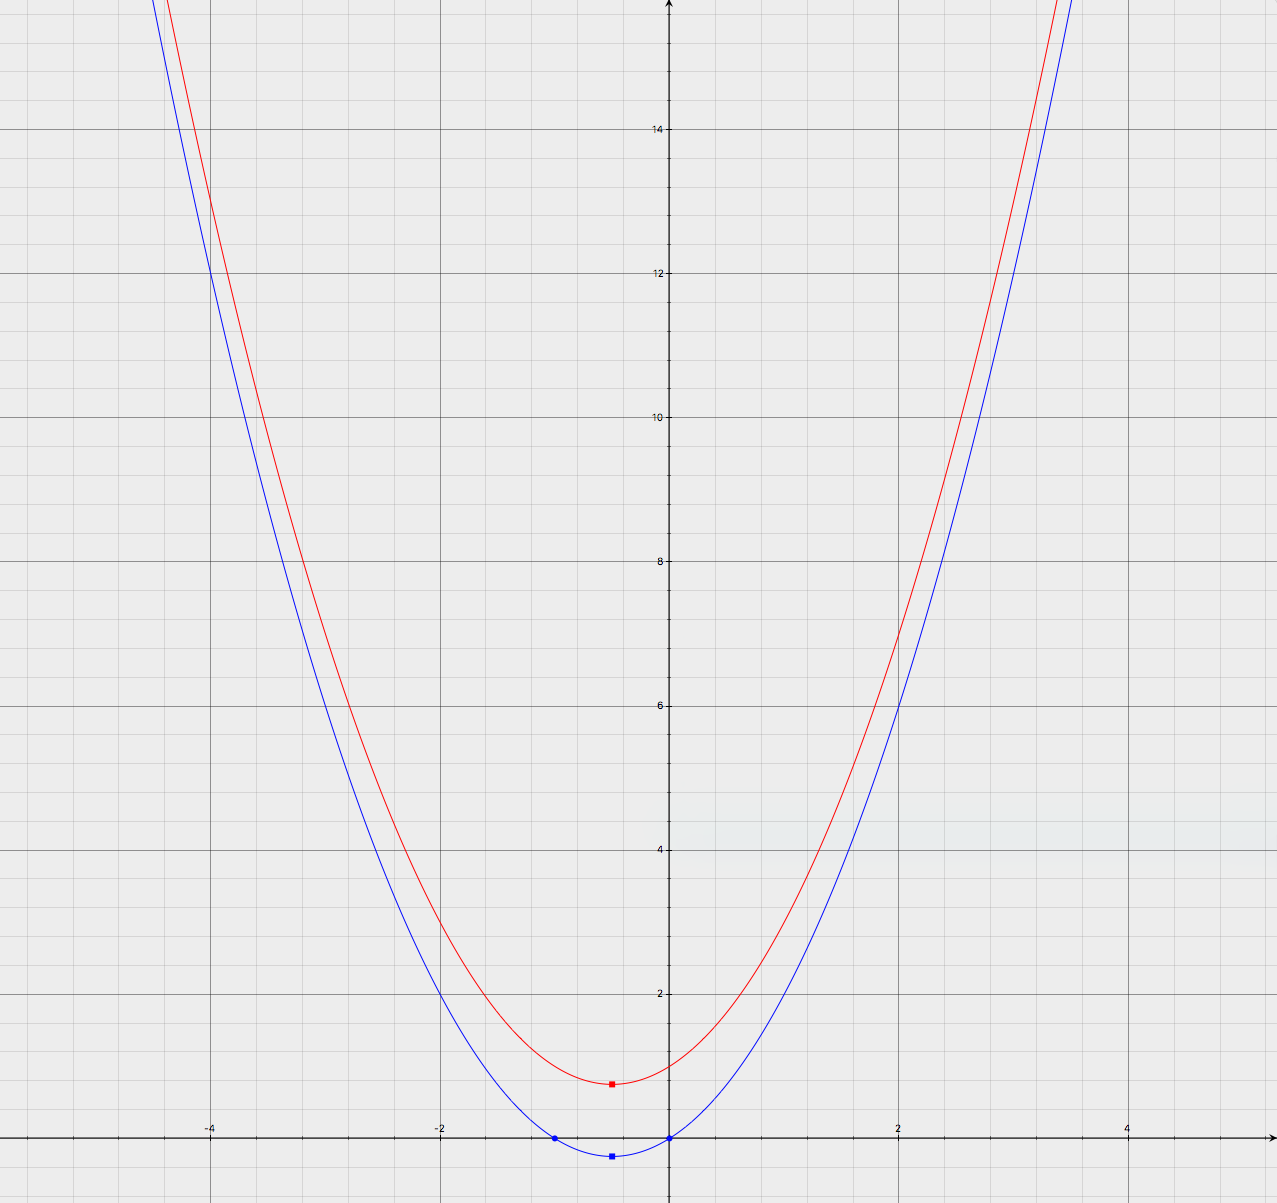
\includegraphics[width=0.5\textwidth]{img/curve-approximation.png}
\label{figure:curve-approximation}
\end{figure}

The last parameter is a threshold error, often called \emph{epsilon}. In most problems trying to be solved by any evolutionary algorithm, it will be very hard to achieve an exact solution. However, in all of these problems, a close-enough solution is usually a sufficient solution. For example, take a look at figure \ref{figure:curve-approximation}. We can see two plots, and maybe our target function is represented by the blue line, while our evolved solution is the red one. Maybe this is enough, depending on where we want to use this function. For example, maybe we want to evolve a program that manages the cruise control of a car, and if we do not get an exact solution, the car might go 2 miles per hour faster or slower than our desired speed limit, and this could be a very good solution.

In other cases, any error is unacceptable, such as in determining if a patient requires an amputation or not. Now, epsilon tells the GP algorithm how bad a solution can perform while maintaining us happy with the results. In our example, this error is obtained by calculating the mean-squared error (MSE), which is pretty easy to understand: you only need subtract every simulated data point to each of its real counterpart, sum all of these numbers and average them, and then get that number's square root. If you are wondering why provide both a number of generations and an epsilon, the answer is that the program will stop when any of these criteria are met. These stop criteria can be interpreted as: "I'm willing to wait for 100 generations or until the solution achieves this performance error," and this makes perfect sense once you realize that many optimization problems can take weeks or months to finish.

Having explained all the input parameters, we can now fully understand the single most important line in listing \ref{listing:genetic-programming-example}: \textbf{line \ref{line:evolve-function-call}}. In this line, we can see a call to \textbf{evolve}, which will contain all of the previously discussed input parameters. In order, we are sending: the function to be evolved (\emph{target}), the operators to be used in the evolutionary process (\emph{fnBag}), the inputs (\emph{inps}), the outputs (\emph{outs}), the limit number of expressions our evolved function can have, the number of generations the algorithm will run, and epsilon or the good-enough error.

After waiting a few milliseconds (it's an extremely easy problem to solve, after all), we will have a \textbf{simFn} filled with expressions that will hopefully simulate the target function $f(x) = x^2 + x$. To test this, we can evaluate the evolved function with each of the inputs (the integers from -10 to 10), and check if these outputs correspond to the outputs from the target function. This testing is performed at \textbf{lines \ref{line:gp-start-testing}-\ref{line:gp-end-testing}}.

\begin{appendices}
%\appendix
%\appendixname{A}
\chapter{Installing CX}
\index{installing CX}

% \begin{remark}
% Section Outline
%     \begin{itemize}
%     	\item Explain there is a script for installation, which is in beta
%         \item Explain the steps (each of the steps in the script)
%         \item Explain special case in Windows
%         \item Explain you need OpenGL libraries in Ubuntu
%         \item Run tests, run examples (show command line, running the examples)
%     \end{itemize}
% \end{remark}

Eventually, we will have a bootstrapped version of CX, and you'll be able to compile CX using CX, but in the meantime, you need to have a working installation of the Go language to compile CX, as CX is implemented in Go. Although providing instructions on how to install Go is out of the scope of this book, we will give you some guidelines:

\begin{itemize}
\item At the time of writing, you can find instructions on how to install Go here: \url{https://golang.org/doc/install}
\item Make sure you get a version of Go superior to 1.8
\item Correctly setting a Go environment -- particularly the GOPATH variable -- usually decreases the chances of getting errors with the installation of CX
\end{itemize}

After getting your Go installation ready, you will need to install some libraries or programs, depending on your operating system.

In the case of Linux distributions, you might need to install some OpenGL libraries, if you have not done so already. CX has been tested in Ubuntu Linux, and the commands to get the required libraries for this distribution are shown in listing \ref{listing:installing-opengl}.

\begin{lstlisting}[caption={Installing required OpenGL libraries in Ubuntu},captionpos=b,label={listing:installing-opengl}]
sudo apt-get install libxi-dev
sudo apt-get install libgl1-mesa-dev
sudo apt-get install libxrandr-dev
sudo apt-get install libxcursor-dev
sudo apt-get install libxinerama-dev
\end{lstlisting}

As there are dozens of Linux distributions, it would be hard to give instructions on how to get the correct libraries for each of them. Nevertheless, using your favorite search engine to find out the names of those libraries for your distribution, and how to install them should be easy.

If you are using Windows, you might only need to install \emph{GCC}. If you already installed GCC through Cygwin, you might run into trouble, as Go apparently does not get along with Cygwin. If you have not installed GCC, you should install it either through \emph{tdm-gcc} (\url{http://tdm-gcc.tdragon.net/}) or Mingw (\url{http://www.mingw.org/}).

At the moment, most users of CX have installed it on MacOS systems, and in all of the cases the installation of the language has been straightforward.

And finally, you'll need \emph{Git} installed, regardless of your operating system. If you find any problems with the installation, we will be grateful if you can open an issue at CX's GitHub repository (\url{https://github.com/skycoin/cx}), so we can improve the installation process!

After going through the steps of installing Go and the required libraries, you should be able to install CX by running either the \emph{cx.sh} (for *nix users) or the \emph{cx.bat} (for Windows users) installation scripts, which can be found in CX's GitHub repository (\url{https://github.com/skycoin/cx}). If you are running a *nix operating system, you can also try the command shown in listing \ref{listing:cx-installation-one-liner}.

\begin{lstlisting}[caption={One-liner CX installation script for *nix systems},captionpos=b,label={listing:cx-installation-one-liner}]
sh <(curl -s https://raw.githubusercontent.com/skycoin/cx/master/cx.sh)
\end{lstlisting}

If everything went well, you should be able to see CX's version printed in your terminal after running \textbf{cx -v}.

\end{appendices}

\newpage

\printindex

\newpage

\printbibliography[heading=subbibliography,notkeyword=this]

\end{document}
ibliography,notkeyword=this]

\end{document}
